\documentclass[twoside]{book}

% Packages required by doxygen
\usepackage{fixltx2e}
\usepackage{calc}
\usepackage{doxygen}
\usepackage[export]{adjustbox} % also loads graphicx
\usepackage{graphicx}
\usepackage[utf8]{inputenc}
\usepackage{makeidx}
\usepackage{multicol}
\usepackage{multirow}
\PassOptionsToPackage{warn}{textcomp}
\usepackage{textcomp}
\usepackage[nointegrals]{wasysym}
\usepackage[table]{xcolor}

% Font selection
\usepackage[T1]{fontenc}
\usepackage[scaled=.90]{helvet}
\usepackage{courier}
\usepackage{amssymb}
\usepackage{sectsty}
\renewcommand{\familydefault}{\sfdefault}
\allsectionsfont{%
  \fontseries{bc}\selectfont%
  \color{darkgray}%
}
\renewcommand{\DoxyLabelFont}{%
  \fontseries{bc}\selectfont%
  \color{darkgray}%
}
\newcommand{\+}{\discretionary{\mbox{\scriptsize$\hookleftarrow$}}{}{}}

% Page & text layout
\usepackage{geometry}
\geometry{%
  a4paper,%
  top=2.5cm,%
  bottom=2.5cm,%
  left=2.5cm,%
  right=2.5cm%
}
\tolerance=750
\hfuzz=15pt
\hbadness=750
\setlength{\emergencystretch}{15pt}
\setlength{\parindent}{0cm}
\setlength{\parskip}{3ex plus 2ex minus 2ex}
\makeatletter
\renewcommand{\paragraph}{%
  \@startsection{paragraph}{4}{0ex}{-1.0ex}{1.0ex}{%
    \normalfont\normalsize\bfseries\SS@parafont%
  }%
}
\renewcommand{\subparagraph}{%
  \@startsection{subparagraph}{5}{0ex}{-1.0ex}{1.0ex}{%
    \normalfont\normalsize\bfseries\SS@subparafont%
  }%
}
\makeatother

% Headers & footers
\usepackage{fancyhdr}
\pagestyle{fancyplain}
\fancyhead[LE]{\fancyplain{}{\bfseries\thepage}}
\fancyhead[CE]{\fancyplain{}{}}
\fancyhead[RE]{\fancyplain{}{\bfseries\leftmark}}
\fancyhead[LO]{\fancyplain{}{\bfseries\rightmark}}
\fancyhead[CO]{\fancyplain{}{}}
\fancyhead[RO]{\fancyplain{}{\bfseries\thepage}}
\fancyfoot[LE]{\fancyplain{}{}}
\fancyfoot[CE]{\fancyplain{}{}}
\fancyfoot[RE]{\fancyplain{}{\bfseries\scriptsize Generated by Doxygen }}
\fancyfoot[LO]{\fancyplain{}{\bfseries\scriptsize Generated by Doxygen }}
\fancyfoot[CO]{\fancyplain{}{}}
\fancyfoot[RO]{\fancyplain{}{}}
\renewcommand{\footrulewidth}{0.4pt}
\renewcommand{\chaptermark}[1]{%
  \markboth{#1}{}%
}
\renewcommand{\sectionmark}[1]{%
  \markright{\thesection\ #1}%
}

% Indices & bibliography
\usepackage{natbib}
\usepackage[titles]{tocloft}
\setcounter{tocdepth}{3}
\setcounter{secnumdepth}{5}
\makeindex

% Hyperlinks (required, but should be loaded last)
\usepackage{ifpdf}
\ifpdf
  \usepackage[pdftex,pagebackref=true]{hyperref}
\else
  \usepackage[ps2pdf,pagebackref=true]{hyperref}
\fi
\hypersetup{%
  colorlinks=true,%
  linkcolor=blue,%
  citecolor=blue,%
  unicode%
}

% Custom commands
\newcommand{\clearemptydoublepage}{%
  \newpage{\pagestyle{empty}\cleardoublepage}%
}

\usepackage{caption}
\captionsetup{labelsep=space,justification=centering,font={bf},singlelinecheck=off,skip=4pt,position=top}

%===== C O N T E N T S =====

\begin{document}

% Titlepage & ToC
\hypersetup{pageanchor=false,
             bookmarksnumbered=true,
             pdfencoding=unicode
            }
\pagenumbering{roman}
\begin{titlepage}
\vspace*{7cm}
\begin{center}%
{\Large vinecopulib \\[1ex]\large 0.\+0.\+1.\+9990 }\\
\vspace*{1cm}
{\large Generated by Doxygen 1.8.11}\\
\end{center}
\end{titlepage}
\clearemptydoublepage
\tableofcontents
\clearemptydoublepage
\pagenumbering{arabic}
\hypersetup{pageanchor=true}

%--- Begin generated contents ---
\chapter{vinecopulib\+: a C++ library for vine copula modeling}
\label{index}\hypertarget{index}{}\begin{DoxyAuthor}{Authors}
Thomas Nagler and Thibault Vatter
\end{DoxyAuthor}
This is the A\+PI documentation for the vinecopulib C++ library. It provides functionality for statistical dependence modeling with bivariate and vine copulas. For a more high-\/level overview see \href{https://github.com/tvatter/vinecopulib/blob/master/README.md}{\tt R\+E\+A\+D\+ME}.\hypertarget{index_license}{}\section{License}\label{index_license}
The M\+IT License (M\+IT)

Copyright © 2017 Thibault Vatter and Thomas Nagler

Permission is hereby granted, free of charge, to any person obtaining a copy of this software and associated documentation files (the “\+Software”), to deal in the Software without restriction, including without limitation the rights to use, copy, modify, merge, publish, distribute, sublicense, and/or sell copies of the Software, and to permit persons to whom the Software is furnished to do so, subject to the following conditions\+:

The above copyright notice and this permission notice shall be included in all copies or substantial portions of the Software.

T\+HE S\+O\+F\+T\+W\+A\+RE IS P\+R\+O\+V\+I\+D\+ED “\+AS I\+S”, W\+I\+T\+H\+O\+UT W\+A\+R\+R\+A\+N\+TY OF A\+NY K\+I\+ND, E\+X\+P\+R\+E\+SS OR I\+M\+P\+L\+I\+ED, I\+N\+C\+L\+U\+D\+I\+NG B\+UT N\+OT L\+I\+M\+I\+T\+ED TO T\+HE W\+A\+R\+R\+A\+N\+T\+I\+ES OF M\+E\+R\+C\+H\+A\+N\+T\+A\+B\+I\+L\+I\+TY, F\+I\+T\+N\+E\+SS F\+OR A P\+A\+R\+T\+I\+C\+U\+L\+AR P\+U\+R\+P\+O\+SE A\+ND N\+O\+N\+I\+N\+F\+R\+I\+N\+G\+E\+M\+E\+NT. IN NO E\+V\+E\+NT S\+H\+A\+LL T\+HE A\+U\+T\+H\+O\+RS OR C\+O\+P\+Y\+R\+I\+G\+HT H\+O\+L\+D\+E\+RS BE L\+I\+A\+B\+LE F\+OR A\+NY C\+L\+A\+IM, D\+A\+M\+A\+G\+ES OR O\+T\+H\+ER L\+I\+A\+B\+I\+L\+I\+TY, W\+H\+E\+T\+H\+ER IN AN A\+C\+T\+I\+ON OF C\+O\+N\+T\+R\+A\+CT, T\+O\+RT OR O\+T\+H\+E\+R\+W\+I\+SE, A\+R\+I\+S\+I\+NG F\+R\+OM, O\+UT OF OR IN C\+O\+N\+N\+E\+C\+T\+I\+ON W\+I\+TH T\+HE S\+O\+F\+T\+W\+A\+RE OR T\+HE U\+SE OR O\+T\+H\+ER D\+E\+A\+L\+I\+N\+GS IN T\+HE S\+O\+F\+T\+W\+A\+RE. 
\chapter{Module Index}
\section{Modules}
Here is a list of all modules\+:\begin{DoxyCompactList}
\item \contentsline{section}{Readers}{\pageref{group__readers}}{}
\end{DoxyCompactList}

\chapter{Hierarchical Index}
\section{Class Hierarchy}
This inheritance list is sorted roughly, but not completely, alphabetically\+:\begin{DoxyCompactList}
\item \contentsline{section}{vinecopulib\+:\+:Bicop}{\pageref{classvinecopulib_1_1_bicop}}{}
\item \contentsline{section}{vinecopulib\+:\+:Fit\+Controls\+Bicop}{\pageref{classvinecopulib_1_1_fit_controls_bicop}}{}
\begin{DoxyCompactList}
\item \contentsline{section}{vinecopulib\+:\+:Fit\+Controls\+Vinecop}{\pageref{classvinecopulib_1_1_fit_controls_vinecop}}{}
\end{DoxyCompactList}
\item \contentsline{section}{vinecopulib\+:\+:R\+Vine\+Structure}{\pageref{classvinecopulib_1_1_r_vine_structure}}{}
\item \contentsline{section}{vinecopulib\+:\+:Triangular\+Array$<$ T $>$}{\pageref{classvinecopulib_1_1_triangular_array}}{}
\item \contentsline{section}{vinecopulib\+:\+:Triangular\+Array$<$ size\+\_\+t $>$}{\pageref{classvinecopulib_1_1_triangular_array}}{}
\item \contentsline{section}{vinecopulib\+:\+:Vinecop}{\pageref{classvinecopulib_1_1_vinecop}}{}
\end{DoxyCompactList}

\chapter{Class Index}
\section{Class List}
Here are the classes, structs, unions and interfaces with brief descriptions\+:\begin{DoxyCompactList}
\item\contentsline{section}{\hyperlink{classvinecopulib_1_1_bicop}{vinecopulib\+::\+Bicop} \\*A class for bivariate copula models }{\pageref{classvinecopulib_1_1_bicop}}{}
\item\contentsline{section}{\hyperlink{classvinecopulib_1_1_fit_controls_bicop}{vinecopulib\+::\+Fit\+Controls\+Bicop} \\*A class for controlling fit of bivariate copula models }{\pageref{classvinecopulib_1_1_fit_controls_bicop}}{}
\item\contentsline{section}{\hyperlink{classvinecopulib_1_1_fit_controls_vinecop}{vinecopulib\+::\+Fit\+Controls\+Vinecop} \\*A class for controlling fit of bivariate copula models }{\pageref{classvinecopulib_1_1_fit_controls_vinecop}}{}
\item\contentsline{section}{\hyperlink{classvinecopulib_1_1_r_vine_matrix}{vinecopulib\+::\+R\+Vine\+Matrix} \\*A class for regular vine matrices }{\pageref{classvinecopulib_1_1_r_vine_matrix}}{}
\item\contentsline{section}{\hyperlink{classvinecopulib_1_1_vinecop}{vinecopulib\+::\+Vinecop} \\*A class for vine copula models }{\pageref{classvinecopulib_1_1_vinecop}}{}
\end{DoxyCompactList}

\chapter{File Index}
\section{File List}
Here is a list of all documented files with brief descriptions\+:\begin{DoxyCompactList}
\item\contentsline{section}{/home/n5/dev/cpp/vinecopulib/include/{\bfseries bicop.\+hpp} }{\pageref{bicop_8hpp}}{}
\item\contentsline{section}{/home/n5/dev/cpp/vinecopulib/include/{\bfseries bicop\+\_\+archimedean.\+hpp} }{\pageref{bicop__archimedean_8hpp}}{}
\item\contentsline{section}{/home/n5/dev/cpp/vinecopulib/include/{\bfseries bicop\+\_\+bb1.\+hpp} }{\pageref{bicop__bb1_8hpp}}{}
\item\contentsline{section}{/home/n5/dev/cpp/vinecopulib/include/{\bfseries bicop\+\_\+bb6.\+hpp} }{\pageref{bicop__bb6_8hpp}}{}
\item\contentsline{section}{/home/n5/dev/cpp/vinecopulib/include/{\bfseries bicop\+\_\+bb7.\+hpp} }{\pageref{bicop__bb7_8hpp}}{}
\item\contentsline{section}{/home/n5/dev/cpp/vinecopulib/include/{\bfseries bicop\+\_\+bb8.\+hpp} }{\pageref{bicop__bb8_8hpp}}{}
\item\contentsline{section}{/home/n5/dev/cpp/vinecopulib/include/{\bfseries bicop\+\_\+class.\+hpp} }{\pageref{bicop__class_8hpp}}{}
\item\contentsline{section}{/home/n5/dev/cpp/vinecopulib/include/{\bfseries bicop\+\_\+clayton.\+hpp} }{\pageref{bicop__clayton_8hpp}}{}
\item\contentsline{section}{/home/n5/dev/cpp/vinecopulib/include/{\bfseries bicop\+\_\+elliptical.\+hpp} }{\pageref{bicop__elliptical_8hpp}}{}
\item\contentsline{section}{/home/n5/dev/cpp/vinecopulib/include/{\bfseries bicop\+\_\+family.\+hpp} }{\pageref{bicop__family_8hpp}}{}
\item\contentsline{section}{/home/n5/dev/cpp/vinecopulib/include/{\bfseries bicop\+\_\+frank.\+hpp} }{\pageref{bicop__frank_8hpp}}{}
\item\contentsline{section}{/home/n5/dev/cpp/vinecopulib/include/{\bfseries bicop\+\_\+gaussian.\+hpp} }{\pageref{bicop__gaussian_8hpp}}{}
\item\contentsline{section}{/home/n5/dev/cpp/vinecopulib/include/{\bfseries bicop\+\_\+gumbel.\+hpp} }{\pageref{bicop__gumbel_8hpp}}{}
\item\contentsline{section}{/home/n5/dev/cpp/vinecopulib/include/{\bfseries bicop\+\_\+indep.\+hpp} }{\pageref{bicop__indep_8hpp}}{}
\item\contentsline{section}{/home/n5/dev/cpp/vinecopulib/include/{\bfseries bicop\+\_\+joe.\+hpp} }{\pageref{bicop__joe_8hpp}}{}
\item\contentsline{section}{/home/n5/dev/cpp/vinecopulib/include/{\bfseries bicop\+\_\+kernel.\+hpp} }{\pageref{bicop__kernel_8hpp}}{}
\item\contentsline{section}{/home/n5/dev/cpp/vinecopulib/include/{\bfseries bicop\+\_\+parametric.\+hpp} }{\pageref{bicop__parametric_8hpp}}{}
\item\contentsline{section}{/home/n5/dev/cpp/vinecopulib/include/{\bfseries bicop\+\_\+student.\+hpp} }{\pageref{bicop__student_8hpp}}{}
\item\contentsline{section}{/home/n5/dev/cpp/vinecopulib/include/{\bfseries bicop\+\_\+trafokernel.\+hpp} }{\pageref{bicop__trafokernel_8hpp}}{}
\item\contentsline{section}{/home/n5/dev/cpp/vinecopulib/include/{\bfseries interpolation\+\_\+grid.\+hpp} }{\pageref{interpolation__grid_8hpp}}{}
\item\contentsline{section}{/home/n5/dev/cpp/vinecopulib/include/\hyperlink{mainpage_8h}{mainpage.\+h} \\*Api\+\_\+docs }{\pageref{mainpage_8h}}{}
\item\contentsline{section}{/home/n5/dev/cpp/vinecopulib/include/{\bfseries rvine\+\_\+matrix.\+hpp} }{\pageref{rvine__matrix_8hpp}}{}
\item\contentsline{section}{/home/n5/dev/cpp/vinecopulib/include/{\bfseries tools\+\_\+bicopselect.\+hpp} }{\pageref{tools__bicopselect_8hpp}}{}
\item\contentsline{section}{/home/n5/dev/cpp/vinecopulib/include/{\bfseries tools\+\_\+eigen.\+hpp} }{\pageref{tools__eigen_8hpp}}{}
\item\contentsline{section}{/home/n5/dev/cpp/vinecopulib/include/{\bfseries tools\+\_\+integration.\+hpp} }{\pageref{tools__integration_8hpp}}{}
\item\contentsline{section}{/home/n5/dev/cpp/vinecopulib/include/{\bfseries tools\+\_\+optimization.\+hpp} }{\pageref{tools__optimization_8hpp}}{}
\item\contentsline{section}{/home/n5/dev/cpp/vinecopulib/include/{\bfseries tools\+\_\+stats.\+hpp} }{\pageref{tools__stats_8hpp}}{}
\item\contentsline{section}{/home/n5/dev/cpp/vinecopulib/include/{\bfseries tools\+\_\+stl.\+hpp} }{\pageref{tools__stl_8hpp}}{}
\item\contentsline{section}{/home/n5/dev/cpp/vinecopulib/include/{\bfseries tools\+\_\+structselect.\+hpp} }{\pageref{tools__structselect_8hpp}}{}
\item\contentsline{section}{/home/n5/dev/cpp/vinecopulib/include/{\bfseries vinecop\+\_\+class.\+hpp} }{\pageref{vinecop__class_8hpp}}{}
\end{DoxyCompactList}

\chapter{Module Documentation}
\hypertarget{group__hfunctions}{}\section{h-\/functions}
\label{group__hfunctions}\index{h-\/functions@{h-\/functions}}
\subsection*{Functions}
\begin{DoxyCompactItemize}
\item 
Eigen\+::\+Vector\+Xd {\bfseries vinecopulib\+::\+Bicop\+::hfunc1} (const Eigen\+::\+Matrix$<$ double, Eigen\+::\+Dynamic, 2 $>$ \&u)\hypertarget{group__hfunctions_ga130fda62cd61c7acdef5db75fffdd89e}{}\label{group__hfunctions_ga130fda62cd61c7acdef5db75fffdd89e}

\item 
Eigen\+::\+Vector\+Xd {\bfseries vinecopulib\+::\+Bicop\+::hfunc2} (const Eigen\+::\+Matrix$<$ double, Eigen\+::\+Dynamic, 2 $>$ \&u)\hypertarget{group__hfunctions_ga4c9b50f99797ec374f5057cc54db2bd8}{}\label{group__hfunctions_ga4c9b50f99797ec374f5057cc54db2bd8}

\item 
Eigen\+::\+Vector\+Xd {\bfseries vinecopulib\+::\+Bicop\+::hinv1} (const Eigen\+::\+Matrix$<$ double, Eigen\+::\+Dynamic, 2 $>$ \&u)\hypertarget{group__hfunctions_ga3cc8b161ec6efdb3b34d2efa9185bf44}{}\label{group__hfunctions_ga3cc8b161ec6efdb3b34d2efa9185bf44}

\item 
Eigen\+::\+Vector\+Xd {\bfseries vinecopulib\+::\+Bicop\+::hinv2} (const Eigen\+::\+Matrix$<$ double, Eigen\+::\+Dynamic, 2 $>$ \&u)\hypertarget{group__hfunctions_ga3e33ec227b6b7182e327399201cad382}{}\label{group__hfunctions_ga3e33ec227b6b7182e327399201cad382}

\end{DoxyCompactItemize}


\subsection{Detailed Description}
h-\/functions are defined as one-\/dimensional integrals over a bivariate copula density $ c $, \[ h_1(u_1, u_2) = \int_0^{u_2} c(u_1, s) ds, \] \[ h_2(u_1, u_2) = \int_0^{u_1} c(s, u_2) ds. \] {\ttfamily hinv1} is the inverse w.\+r.\+t. second argument (conditioned on first), {\ttfamily hinv2} is the inverse w.\+r.\+t. first argument (conditioned on second),

{\ttfamily hfunc1}, {\ttfamily hfunc2}, {\ttfamily hinv1}, and {\ttfamily hinv2} mainly take care that rotations are properly handled. They call {\ttfamily hfunc1\+\_\+default}, {\ttfamily hfunc2\+\_\+default}, {\ttfamily hinv1\+\_\+default}, and hinv2\+\_\+default which are family-\/specific implementations for {\ttfamily rotation = 0}.


\begin{DoxyParams}{Parameters}
{\em u} & $m \times 2$ matrix of evaluation points. \\
\hline
\end{DoxyParams}
\begin{DoxyReturn}{Returns}
The (inverse) h-\/function evaluated at {\ttfamily u}. 
\end{DoxyReturn}

\chapter{Class Documentation}
\hypertarget{classvinecopulib_1_1_archimedean_bicop}{\section{vinecopulib\+:\+:Archimedean\+Bicop Class Reference}
\label{classvinecopulib_1_1_archimedean_bicop}\index{vinecopulib\+::\+Archimedean\+Bicop@{vinecopulib\+::\+Archimedean\+Bicop}}
}


An abstract class for Archimedean copula families.  




{\ttfamily \#include $<$archimedean.\+hpp$>$}



Inheritance diagram for vinecopulib\+:\+:Archimedean\+Bicop\+:\nopagebreak
\begin{figure}[H]
\begin{center}
\leavevmode
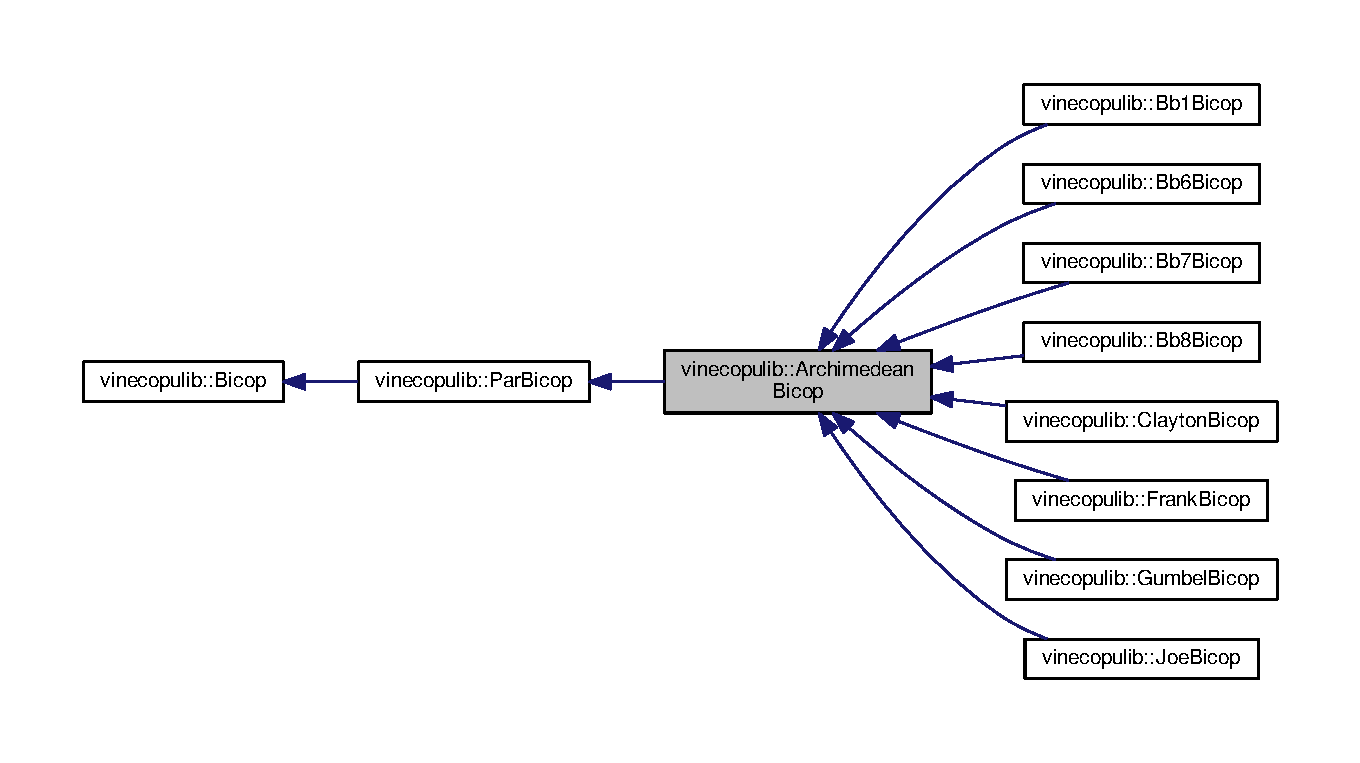
\includegraphics[width=350pt]{classvinecopulib_1_1_archimedean_bicop__inherit__graph}
\end{center}
\end{figure}


Collaboration diagram for vinecopulib\+:\+:Archimedean\+Bicop\+:\nopagebreak
\begin{figure}[H]
\begin{center}
\leavevmode
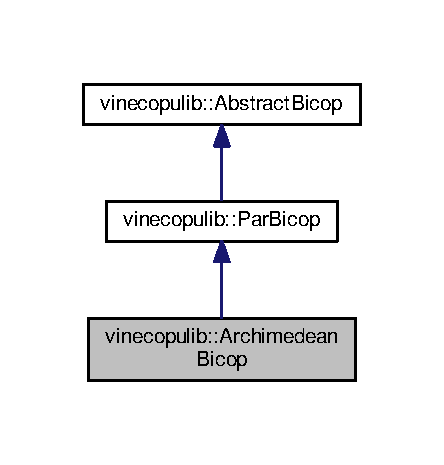
\includegraphics[width=212pt]{classvinecopulib_1_1_archimedean_bicop__coll__graph}
\end{center}
\end{figure}
\subsection*{Additional Inherited Members}


\subsection{Detailed Description}
An abstract class for Archimedean copula families. 

This class is used in the implementation underlying the \hyperlink{classvinecopulib_1_1_bicop}{Bicop} class. Users should not use \hyperlink{classvinecopulib_1_1_abstract_bicop}{Abstract\+Bicop} or derived classes directly, but always work with the \hyperlink{classvinecopulib_1_1_bicop}{Bicop} interface.

Joe, Harry. Dependence modeling with copulas. C\+R\+C Press, 2014. 

The documentation for this class was generated from the following files\+:\begin{DoxyCompactItemize}
\item 
vinecopulib/include/vinecopulib/bicop/archimedean.\+hpp\item 
vinecopulib/src/bicop/archimedean.\+cpp\end{DoxyCompactItemize}

\hypertarget{classvinecopulib_1_1_bb1_bicop}{\section{vinecopulib\+:\+:Bb1\+Bicop Class Reference}
\label{classvinecopulib_1_1_bb1_bicop}\index{vinecopulib\+::\+Bb1\+Bicop@{vinecopulib\+::\+Bb1\+Bicop}}
}


The B\+B1 copula.  




{\ttfamily \#include $<$bb1.\+hpp$>$}



Inheritance diagram for vinecopulib\+:\+:Bb1\+Bicop\+:\nopagebreak
\begin{figure}[H]
\begin{center}
\leavevmode
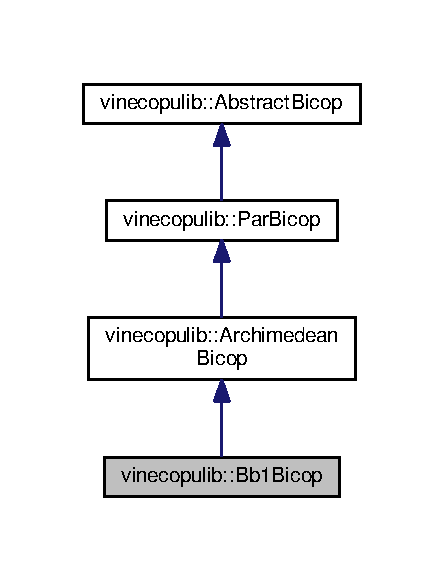
\includegraphics[width=212pt]{classvinecopulib_1_1_bb1_bicop__inherit__graph}
\end{center}
\end{figure}


Collaboration diagram for vinecopulib\+:\+:Bb1\+Bicop\+:\nopagebreak
\begin{figure}[H]
\begin{center}
\leavevmode
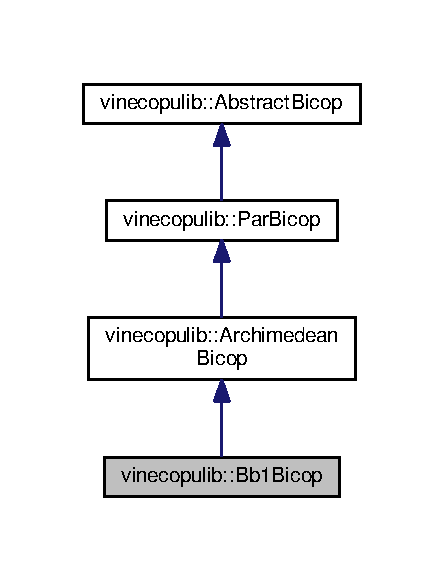
\includegraphics[width=212pt]{classvinecopulib_1_1_bb1_bicop__coll__graph}
\end{center}
\end{figure}
\subsection*{Additional Inherited Members}


\subsection{Detailed Description}
The B\+B1 copula. 

This class is used in the implementation underlying the \hyperlink{classvinecopulib_1_1_bicop}{Bicop} class. Users should not use \hyperlink{classvinecopulib_1_1_abstract_bicop}{Abstract\+Bicop} or derived classes directly, but always work with the \hyperlink{classvinecopulib_1_1_bicop}{Bicop} interface.

Joe, Harry. Dependence modeling with copulas. C\+R\+C Press, 2014. 

The documentation for this class was generated from the following files\+:\begin{DoxyCompactItemize}
\item 
vinecopulib/include/vinecopulib/bicop/bb1.\+hpp\item 
vinecopulib/src/bicop/bb1.\+cpp\end{DoxyCompactItemize}

\hypertarget{classvinecopulib_1_1_bb6_bicop}{}\section{vinecopulib\+:\+:Bb6\+Bicop Class Reference}
\label{classvinecopulib_1_1_bb6_bicop}\index{vinecopulib\+::\+Bb6\+Bicop@{vinecopulib\+::\+Bb6\+Bicop}}


The B\+B6 copula.  




{\ttfamily \#include $<$bb6.\+hpp$>$}



Inheritance diagram for vinecopulib\+:\+:Bb6\+Bicop\+:\nopagebreak
\begin{figure}[H]
\begin{center}
\leavevmode
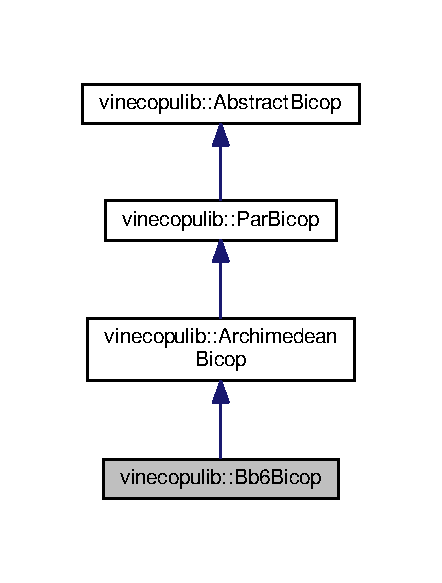
\includegraphics[width=213pt]{classvinecopulib_1_1_bb6_bicop__inherit__graph}
\end{center}
\end{figure}


Collaboration diagram for vinecopulib\+:\+:Bb6\+Bicop\+:\nopagebreak
\begin{figure}[H]
\begin{center}
\leavevmode
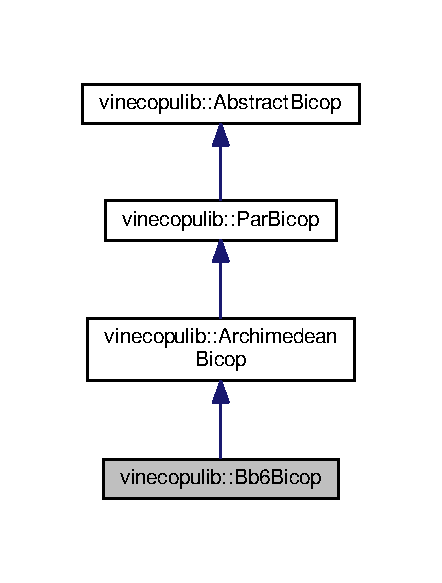
\includegraphics[width=213pt]{classvinecopulib_1_1_bb6_bicop__coll__graph}
\end{center}
\end{figure}
\subsection*{Additional Inherited Members}


\subsection{Detailed Description}
The B\+B6 copula. 

This class is used in the implementation underlying the \hyperlink{classvinecopulib_1_1_bicop}{Bicop} class. Users should not use \hyperlink{classvinecopulib_1_1_abstract_bicop}{Abstract\+Bicop} or derived classes directly, but always work with the \hyperlink{classvinecopulib_1_1_bicop}{Bicop} interface.

Joe, Harry. Dependence modeling with copulas. C\+RC Press, 2014. 

The documentation for this class was generated from the following files\+:\begin{DoxyCompactItemize}
\item 
/home/n5/dev/cpp/vinecopulib/include/vinecopulib/bicop/bb6.\+hpp\item 
/home/n5/dev/cpp/vinecopulib/src/bicop/bb6.\+cpp\end{DoxyCompactItemize}

\hypertarget{classvinecopulib_1_1_bb7_bicop}{}\section{vinecopulib\+:\+:Bb7\+Bicop Class Reference}
\label{classvinecopulib_1_1_bb7_bicop}\index{vinecopulib\+::\+Bb7\+Bicop@{vinecopulib\+::\+Bb7\+Bicop}}


The B\+B7 copula.  




{\ttfamily \#include $<$bb7.\+hpp$>$}



Inheritance diagram for vinecopulib\+:\+:Bb7\+Bicop\+:\nopagebreak
\begin{figure}[H]
\begin{center}
\leavevmode
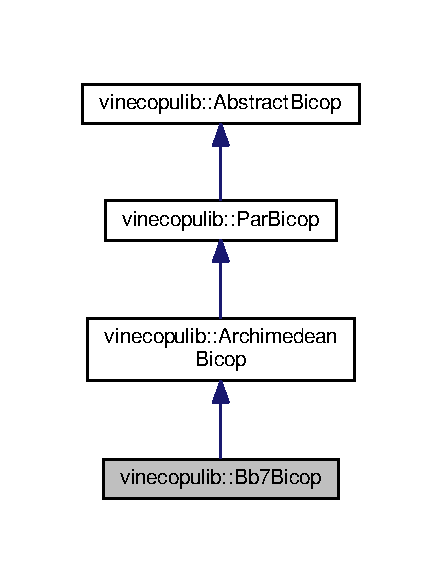
\includegraphics[width=213pt]{classvinecopulib_1_1_bb7_bicop__inherit__graph}
\end{center}
\end{figure}


Collaboration diagram for vinecopulib\+:\+:Bb7\+Bicop\+:\nopagebreak
\begin{figure}[H]
\begin{center}
\leavevmode
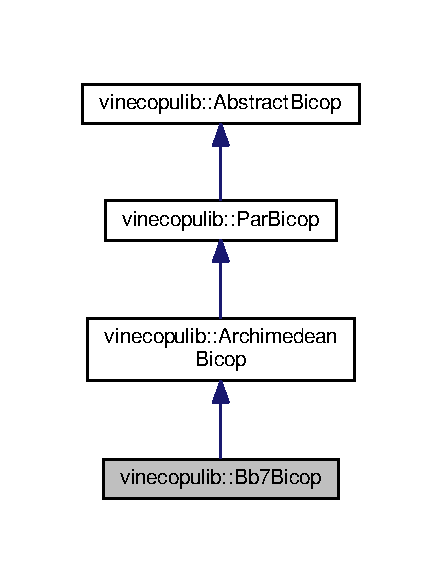
\includegraphics[width=213pt]{classvinecopulib_1_1_bb7_bicop__coll__graph}
\end{center}
\end{figure}
\subsection*{Additional Inherited Members}


\subsection{Detailed Description}
The B\+B7 copula. 

This class is used in the implementation underlying the \hyperlink{classvinecopulib_1_1_bicop}{Bicop} class. Users should not use \hyperlink{classvinecopulib_1_1_abstract_bicop}{Abstract\+Bicop} or derived classes directly, but always work with the \hyperlink{classvinecopulib_1_1_bicop}{Bicop} interface.

Joe, Harry. Dependence modeling with copulas. C\+RC Press, 2014. 

The documentation for this class was generated from the following files\+:\begin{DoxyCompactItemize}
\item 
/home/n5/dev/cpp/vinecopulib/include/vinecopulib/bicop/bb7.\+hpp\item 
/home/n5/dev/cpp/vinecopulib/src/bicop/bb7.\+cpp\end{DoxyCompactItemize}

\hypertarget{classvinecopulib_1_1_bb8_bicop}{}\section{vinecopulib\+:\+:Bb8\+Bicop Class Reference}
\label{classvinecopulib_1_1_bb8_bicop}\index{vinecopulib\+::\+Bb8\+Bicop@{vinecopulib\+::\+Bb8\+Bicop}}


Inheritance diagram for vinecopulib\+:\+:Bb8\+Bicop\+:\nopagebreak
\begin{figure}[H]
\begin{center}
\leavevmode
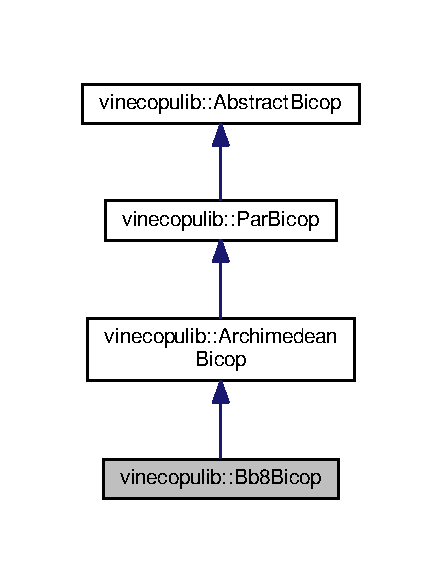
\includegraphics[width=208pt]{classvinecopulib_1_1_bb8_bicop__inherit__graph}
\end{center}
\end{figure}


Collaboration diagram for vinecopulib\+:\+:Bb8\+Bicop\+:\nopagebreak
\begin{figure}[H]
\begin{center}
\leavevmode
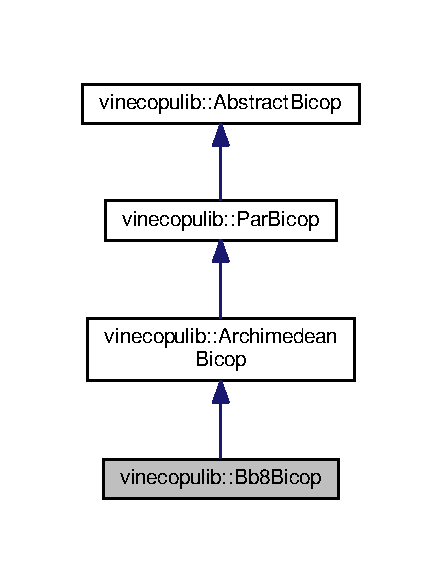
\includegraphics[width=208pt]{classvinecopulib_1_1_bb8_bicop__coll__graph}
\end{center}
\end{figure}
\subsection*{Additional Inherited Members}


The documentation for this class was generated from the following files\+:\begin{DoxyCompactItemize}
\item 
/home/n5/dev/cpp/vinecopulib/include/bicop\+\_\+bb8.\+hpp\item 
/home/n5/dev/cpp/vinecopulib/src/bicop\+\_\+bb8.\+cpp\end{DoxyCompactItemize}

\hypertarget{classvinecopulib_1_1_bicop}{}\section{vinecopulib\+:\+:Bicop Class Reference}
\label{classvinecopulib_1_1_bicop}\index{vinecopulib\+::\+Bicop@{vinecopulib\+::\+Bicop}}


A class for bivariate copula models.  




{\ttfamily \#include $<$class.\+hpp$>$}

\subsection*{Public Member Functions}
\begin{DoxyCompactItemize}
\item 
\hyperlink{classvinecopulib_1_1_bicop_acfa522fb0bea4aca8fade87c18bcf921}{Bicop} ()\hypertarget{classvinecopulib_1_1_bicop_acfa522fb0bea4aca8fade87c18bcf921}{}\label{classvinecopulib_1_1_bicop_acfa522fb0bea4aca8fade87c18bcf921}

\begin{DoxyCompactList}\small\item\em creates the independence copula. \end{DoxyCompactList}\item 
\hyperlink{classvinecopulib_1_1_bicop_ab27f789e001e30f2fed7f9ecefdeffb0}{Bicop} (\hyperlink{namespacevinecopulib_a42e95cc06d33896199caab0c11ad44f3}{Bicop\+Family} family, int rotation=0, const Eigen\+::\+Matrix\+Xd \&parameters=Eigen\+::\+Matrix\+Xd())
\item 
\hyperlink{classvinecopulib_1_1_bicop_a87d5c10cb7b6a9c07dc3b2a38da91ee5}{Bicop} (Eigen\+::\+Matrix$<$ double, Eigen\+::\+Dynamic, 2 $>$ data, std\+::vector$<$ \hyperlink{namespacevinecopulib_a42e95cc06d33896199caab0c11ad44f3}{Bicop\+Family} $>$ family\+\_\+set=\hyperlink{namespacevinecopulib_1_1bicop__families_a5214a513f41ec23b74782aab96ea6774}{bicop\+\_\+families\+::all}, std\+::string method=\char`\"{}mle\char`\"{}, std\+::string selection\+\_\+criterion=\char`\"{}bic\char`\"{}, bool preselect\+\_\+families=true)
\item 
Eigen\+::\+Vector\+Xd \hyperlink{classvinecopulib_1_1_bicop_a83dc7214e4bb1bfe59285ca05407d646}{pdf} (const Eigen\+::\+Matrix$<$ double, Eigen\+::\+Dynamic, 2 $>$ \&u)
\item 
Eigen\+::\+Vector\+Xd \hyperlink{classvinecopulib_1_1_bicop_a130fda62cd61c7acdef5db75fffdd89e}{hfunc1} (const Eigen\+::\+Matrix$<$ double, Eigen\+::\+Dynamic, 2 $>$ \&u)
\item 
Eigen\+::\+Vector\+Xd \hyperlink{classvinecopulib_1_1_bicop_a4c9b50f99797ec374f5057cc54db2bd8}{hfunc2} (const Eigen\+::\+Matrix$<$ double, Eigen\+::\+Dynamic, 2 $>$ \&u)
\item 
Eigen\+::\+Vector\+Xd \hyperlink{classvinecopulib_1_1_bicop_a3cc8b161ec6efdb3b34d2efa9185bf44}{hinv1} (const Eigen\+::\+Matrix$<$ double, Eigen\+::\+Dynamic, 2 $>$ \&u)
\item 
Eigen\+::\+Vector\+Xd \hyperlink{classvinecopulib_1_1_bicop_a3e33ec227b6b7182e327399201cad382}{hinv2} (const Eigen\+::\+Matrix$<$ double, Eigen\+::\+Dynamic, 2 $>$ \&u)
\item 
Eigen\+::\+Matrix$<$ double, Eigen\+::\+Dynamic, 2 $>$ \hyperlink{classvinecopulib_1_1_bicop_aeb87bea4283dacfa5e609356c020f85d}{simulate} (const int \&n)
\item 
void \hyperlink{classvinecopulib_1_1_bicop_a266fa8d13e8ed1e96937e4208a99955d}{fit} (const Eigen\+::\+Matrix$<$ double, Eigen\+::\+Dynamic, 2 $>$ \&data, std\+::string method)
\item 
void \hyperlink{classvinecopulib_1_1_bicop_af04ef20ec08d02222059ba2b72084ad0}{select} (Eigen\+::\+Matrix$<$ double, Eigen\+::\+Dynamic, 2 $>$ data, std\+::vector$<$ \hyperlink{namespacevinecopulib_a42e95cc06d33896199caab0c11ad44f3}{Bicop\+Family} $>$ family\+\_\+set=\hyperlink{namespacevinecopulib_1_1bicop__families_a5214a513f41ec23b74782aab96ea6774}{bicop\+\_\+families\+::all}, std\+::string method=\char`\"{}mle\char`\"{}, std\+::string selection\+\_\+criterion=\char`\"{}bic\char`\"{}, bool preselect\+\_\+families=true)
\item 
double \hyperlink{classvinecopulib_1_1_bicop_ae8bcc0c3265cc86565333a0cfd3d619d}{loglik} (const Eigen\+::\+Matrix$<$ double, Eigen\+::\+Dynamic, 2 $>$ \&u)
\item 
double \hyperlink{classvinecopulib_1_1_bicop_a9287fec95519fea64a2ae80f5888c709}{aic} (const Eigen\+::\+Matrix$<$ double, Eigen\+::\+Dynamic, 2 $>$ \&u)
\item 
double \hyperlink{classvinecopulib_1_1_bicop_ac1f480d13b3464260c2dd6aa88b2e130}{bic} (const Eigen\+::\+Matrix$<$ double, Eigen\+::\+Dynamic, 2 $>$ \&u)
\item 
double \hyperlink{classvinecopulib_1_1_bicop_a9f3b3b83c54a9e1d809fdee058f3eb11}{calculate\+\_\+npars} ()
\item 
double \hyperlink{classvinecopulib_1_1_bicop_aa25436353dee76e4368fb941a7efa257}{parameters\+\_\+to\+\_\+tau} (const Eigen\+::\+Vector\+Xd \&parameters)
\item 
Eigen\+::\+Matrix\+Xd \hyperlink{classvinecopulib_1_1_bicop_a5809ddc9884f6fb66fe53289be348913}{tau\+\_\+to\+\_\+parameters} (const double \&tau)
\end{DoxyCompactItemize}
\begin{Indent}{\bf Getters and setters}\par
\begin{DoxyCompactItemize}
\item 
\hyperlink{namespacevinecopulib_a42e95cc06d33896199caab0c11ad44f3}{Bicop\+Family} {\bfseries get\+\_\+family} () const \hypertarget{classvinecopulib_1_1_bicop_a68ab3556ee3bb3d02814fd978573bf3b}{}\label{classvinecopulib_1_1_bicop_a68ab3556ee3bb3d02814fd978573bf3b}

\item 
std\+::string {\bfseries get\+\_\+family\+\_\+name} () const \hypertarget{classvinecopulib_1_1_bicop_a4d4fbc0fdca17564c23f4814d5d2fbe7}{}\label{classvinecopulib_1_1_bicop_a4d4fbc0fdca17564c23f4814d5d2fbe7}

\item 
int {\bfseries get\+\_\+rotation} () const \hypertarget{classvinecopulib_1_1_bicop_ab8e52577a50fbfc57277f9240d8eac03}{}\label{classvinecopulib_1_1_bicop_ab8e52577a50fbfc57277f9240d8eac03}

\item 
Eigen\+::\+Matrix\+Xd {\bfseries get\+\_\+parameters} () const \hypertarget{classvinecopulib_1_1_bicop_a93ab0dd89826e50b209ea3760f251f2f}{}\label{classvinecopulib_1_1_bicop_a93ab0dd89826e50b209ea3760f251f2f}

\item 
void \hyperlink{classvinecopulib_1_1_bicop_a4e359624560a089273b25dc74879bd16}{set\+\_\+rotation} (int rotation)
\item 
void \hyperlink{classvinecopulib_1_1_bicop_ac8d1d4266b0fd7e2f971d0149f881ef9}{set\+\_\+parameters} (const Eigen\+::\+Matrix\+Xd \&parameters)
\end{DoxyCompactItemize}
\end{Indent}
\begin{Indent}{\bf Utilities}\par
{\em adjust\textquotesingle{}s the copula model to a change in the variable order. }\begin{DoxyCompactItemize}
\item 
std\+::string \hyperlink{classvinecopulib_1_1_bicop_a94b889d56f478dbeb156be4e31af5de5}{str} ()\hypertarget{classvinecopulib_1_1_bicop_a94b889d56f478dbeb156be4e31af5de5}{}\label{classvinecopulib_1_1_bicop_a94b889d56f478dbeb156be4e31af5de5}

\begin{DoxyCompactList}\small\item\em summarizes the model into a string (can be used for printing). \end{DoxyCompactList}\item 
void {\bfseries flip} ()\hypertarget{classvinecopulib_1_1_bicop_a59b7087b3857350df25ff684ab96f377}{}\label{classvinecopulib_1_1_bicop_a59b7087b3857350df25ff684ab96f377}

\end{DoxyCompactItemize}
\end{Indent}


\subsection{Detailed Description}
A class for bivariate copula models. 

The copula model is fully characterized by the family, rotation, and parameters. 

\subsection{Constructor \& Destructor Documentation}
\index{vinecopulib\+::\+Bicop@{vinecopulib\+::\+Bicop}!Bicop@{Bicop}}
\index{Bicop@{Bicop}!vinecopulib\+::\+Bicop@{vinecopulib\+::\+Bicop}}
\subsubsection[{\texorpdfstring{Bicop(\+Bicop\+Family family, int rotation=0, const Eigen\+::\+Matrix\+Xd \&parameters=\+Eigen\+::\+Matrix\+Xd())}{Bicop(BicopFamily family, int rotation=0, const Eigen::MatrixXd &parameters=Eigen::MatrixXd())}}]{\setlength{\rightskip}{0pt plus 5cm}vinecopulib\+::\+Bicop\+::\+Bicop (
\begin{DoxyParamCaption}
\item[{{\bf Bicop\+Family}}]{family, }
\item[{int}]{rotation = {\ttfamily 0}, }
\item[{const Eigen\+::\+Matrix\+Xd \&}]{parameters = {\ttfamily Eigen\+:\+:MatrixXd()}}
\end{DoxyParamCaption}
)}\hypertarget{classvinecopulib_1_1_bicop_ab27f789e001e30f2fed7f9ecefdeffb0}{}\label{classvinecopulib_1_1_bicop_ab27f789e001e30f2fed7f9ecefdeffb0}
creates a specific bivariate copula model. 
\begin{DoxyParams}{Parameters}
{\em family} & the copula family. \\
\hline
{\em rotation} & the rotation of the copula; one of 0, 90, 180, or 270 (for Independence, Gaussian, Student, Frank, and nonparametric families, only 0 is allowed). \\
\hline
{\em parameters} & the copula parameters. \\
\hline
\end{DoxyParams}
\index{vinecopulib\+::\+Bicop@{vinecopulib\+::\+Bicop}!Bicop@{Bicop}}
\index{Bicop@{Bicop}!vinecopulib\+::\+Bicop@{vinecopulib\+::\+Bicop}}
\subsubsection[{\texorpdfstring{Bicop(\+Eigen\+::\+Matrix$<$ double, Eigen\+::\+Dynamic, 2 $>$ data, std\+::vector$<$ Bicop\+Family $>$ family\+\_\+set=bicop\+\_\+families\+::all, std\+::string method=""mle"", std\+::string selection\+\_\+criterion=""bic"", bool preselect\+\_\+families=true)}{Bicop(Eigen::Matrix< double, Eigen::Dynamic, 2 > data, std::vector< BicopFamily > family_set=bicop_families::all, std::string method="mle", std::string selection_criterion="bic", bool preselect_families=true)}}]{\setlength{\rightskip}{0pt plus 5cm}vinecopulib\+::\+Bicop\+::\+Bicop (
\begin{DoxyParamCaption}
\item[{Eigen\+::\+Matrix$<$ double, Eigen\+::\+Dynamic, 2 $>$}]{data, }
\item[{std\+::vector$<$ {\bf Bicop\+Family} $>$}]{family\+\_\+set = {\ttfamily {\bf bicop\+\_\+families\+::all}}, }
\item[{std\+::string}]{method = {\ttfamily \char`\"{}mle\char`\"{}}, }
\item[{std\+::string}]{selection\+\_\+criterion = {\ttfamily \char`\"{}bic\char`\"{}}, }
\item[{bool}]{preselect\+\_\+families = {\ttfamily true}}
\end{DoxyParamCaption}
)}\hypertarget{classvinecopulib_1_1_bicop_a87d5c10cb7b6a9c07dc3b2a38da91ee5}{}\label{classvinecopulib_1_1_bicop_a87d5c10cb7b6a9c07dc3b2a38da91ee5}
equivalent to {\ttfamily \hyperlink{classvinecopulib_1_1_bicop}{Bicop} cop; cop.\+select(data, family\+\_\+set, ...)}. 
\begin{DoxyParams}{Parameters}
{\em data} & see \hyperlink{classvinecopulib_1_1_bicop_af04ef20ec08d02222059ba2b72084ad0}{select()}. \\
\hline
{\em family\+\_\+set} & see \hyperlink{classvinecopulib_1_1_bicop_af04ef20ec08d02222059ba2b72084ad0}{select()}. \\
\hline
{\em method} & see \hyperlink{classvinecopulib_1_1_bicop_af04ef20ec08d02222059ba2b72084ad0}{select()}. \\
\hline
{\em selection\+\_\+criterion} & see \hyperlink{classvinecopulib_1_1_bicop_af04ef20ec08d02222059ba2b72084ad0}{select()}. \\
\hline
{\em preselect\+\_\+families} & see \hyperlink{classvinecopulib_1_1_bicop_af04ef20ec08d02222059ba2b72084ad0}{select()}. \\
\hline
\end{DoxyParams}


\subsection{Member Function Documentation}
\index{vinecopulib\+::\+Bicop@{vinecopulib\+::\+Bicop}!aic@{aic}}
\index{aic@{aic}!vinecopulib\+::\+Bicop@{vinecopulib\+::\+Bicop}}
\subsubsection[{\texorpdfstring{aic(const Eigen\+::\+Matrix$<$ double, Eigen\+::\+Dynamic, 2 $>$ \&u)}{aic(const Eigen::Matrix< double, Eigen::Dynamic, 2 > &u)}}]{\setlength{\rightskip}{0pt plus 5cm}double vinecopulib\+::\+Bicop\+::aic (
\begin{DoxyParamCaption}
\item[{const Eigen\+::\+Matrix$<$ double, Eigen\+::\+Dynamic, 2 $>$ \&}]{u}
\end{DoxyParamCaption}
)}\hypertarget{classvinecopulib_1_1_bicop_a9287fec95519fea64a2ae80f5888c709}{}\label{classvinecopulib_1_1_bicop_a9287fec95519fea64a2ae80f5888c709}
calculates the Akaike information criterion (A\+IC).

The A\+IC is defined as \[ \mathrm{AIC} = -2\, \mathrm{loglik} + 2 p, \] where $ \mathrm{loglik} $ is the log-\/liklihood and $ p $ is the (effective) number of parameters of the model, see \hyperlink{classvinecopulib_1_1_bicop_ae8bcc0c3265cc86565333a0cfd3d619d}{loglik()} and \hyperlink{classvinecopulib_1_1_bicop_a9f3b3b83c54a9e1d809fdee058f3eb11}{calculate\+\_\+npars()}. The A\+IC is a consistent model selection criterion for nonparametric models.


\begin{DoxyParams}{Parameters}
{\em u} & $n \times 2$ matrix of observations. \\
\hline
\end{DoxyParams}
\index{vinecopulib\+::\+Bicop@{vinecopulib\+::\+Bicop}!bic@{bic}}
\index{bic@{bic}!vinecopulib\+::\+Bicop@{vinecopulib\+::\+Bicop}}
\subsubsection[{\texorpdfstring{bic(const Eigen\+::\+Matrix$<$ double, Eigen\+::\+Dynamic, 2 $>$ \&u)}{bic(const Eigen::Matrix< double, Eigen::Dynamic, 2 > &u)}}]{\setlength{\rightskip}{0pt plus 5cm}double vinecopulib\+::\+Bicop\+::bic (
\begin{DoxyParamCaption}
\item[{const Eigen\+::\+Matrix$<$ double, Eigen\+::\+Dynamic, 2 $>$ \&}]{u}
\end{DoxyParamCaption}
)}\hypertarget{classvinecopulib_1_1_bicop_ac1f480d13b3464260c2dd6aa88b2e130}{}\label{classvinecopulib_1_1_bicop_ac1f480d13b3464260c2dd6aa88b2e130}
calculates the Bayesian information criterion (B\+IC).

The B\+IC is defined as \[ \mathrm{BIC} = -2\, \mathrm{loglik} + \ln(n) p, \] where $ \mathrm{loglik} $ is the log-\/liklihood and $ p $ is the (effective) number of parameters of the model, see \hyperlink{classvinecopulib_1_1_bicop_ae8bcc0c3265cc86565333a0cfd3d619d}{loglik()} and \hyperlink{classvinecopulib_1_1_bicop_a9f3b3b83c54a9e1d809fdee058f3eb11}{calculate\+\_\+npars()}. The B\+IC is a consistent model selection criterion for nonparametric models.


\begin{DoxyParams}{Parameters}
{\em u} & $n \times 2$ matrix of observations. \\
\hline
\end{DoxyParams}
\index{vinecopulib\+::\+Bicop@{vinecopulib\+::\+Bicop}!calculate\+\_\+npars@{calculate\+\_\+npars}}
\index{calculate\+\_\+npars@{calculate\+\_\+npars}!vinecopulib\+::\+Bicop@{vinecopulib\+::\+Bicop}}
\subsubsection[{\texorpdfstring{calculate\+\_\+npars()}{calculate_npars()}}]{\setlength{\rightskip}{0pt plus 5cm}double vinecopulib\+::\+Bicop\+::calculate\+\_\+npars (
\begin{DoxyParamCaption}
{}
\end{DoxyParamCaption}
)}\hypertarget{classvinecopulib_1_1_bicop_a9f3b3b83c54a9e1d809fdee058f3eb11}{}\label{classvinecopulib_1_1_bicop_a9f3b3b83c54a9e1d809fdee058f3eb11}
calculates the effective number of parameters.

Returns the actual number of parameters for parameteric families. For nonparametric families, there is a conceptually similar definition in the sense that it can be used in the calculation of fit statistics. \index{vinecopulib\+::\+Bicop@{vinecopulib\+::\+Bicop}!fit@{fit}}
\index{fit@{fit}!vinecopulib\+::\+Bicop@{vinecopulib\+::\+Bicop}}
\subsubsection[{\texorpdfstring{fit(const Eigen\+::\+Matrix$<$ double, Eigen\+::\+Dynamic, 2 $>$ \&data, std\+::string method)}{fit(const Eigen::Matrix< double, Eigen::Dynamic, 2 > &data, std::string method)}}]{\setlength{\rightskip}{0pt plus 5cm}void vinecopulib\+::\+Bicop\+::fit (
\begin{DoxyParamCaption}
\item[{const Eigen\+::\+Matrix$<$ double, Eigen\+::\+Dynamic, 2 $>$ \&}]{data, }
\item[{std\+::string}]{method}
\end{DoxyParamCaption}
)}\hypertarget{classvinecopulib_1_1_bicop_a266fa8d13e8ed1e96937e4208a99955d}{}\label{classvinecopulib_1_1_bicop_a266fa8d13e8ed1e96937e4208a99955d}
fits a bivariate copula (with fixed family) to data.

For parametric models, two different methods are available. {\ttfamily \char`\"{}mle\char`\"{}} fits the parameters by maximum-\/likelihood. {\ttfamily \char`\"{}itau\char`\"{}} uses inversion of Kendall\textquotesingle{}s $ \tau $, but is only available for one-\/parameter families and the Student t copula. For the latter, there is a one-\/to-\/one transformation for the first parameter, the second is found by profile likelihood optimization (with accuracy of at least 0.\+5). Nonparametric families have specialized methods, no specification is required.


\begin{DoxyParams}{Parameters}
{\em data} & an $ n \times 2 $ matrix of observations contained in $(0, 1)^2 $. \\
\hline
{\em method} & the fit method; possible choices\+: {\ttfamily \char`\"{}mle\char`\"{}}, {\ttfamily \char`\"{}itau\char`\"{}}. \\
\hline
\end{DoxyParams}
\index{vinecopulib\+::\+Bicop@{vinecopulib\+::\+Bicop}!hfunc1@{hfunc1}}
\index{hfunc1@{hfunc1}!vinecopulib\+::\+Bicop@{vinecopulib\+::\+Bicop}}
\subsubsection[{\texorpdfstring{hfunc1(const Eigen\+::\+Matrix$<$ double, Eigen\+::\+Dynamic, 2 $>$ \&u)}{hfunc1(const Eigen::Matrix< double, Eigen::Dynamic, 2 > &u)}}]{\setlength{\rightskip}{0pt plus 5cm}Eigen\+::\+Vector\+Xd vinecopulib\+::\+Bicop\+::hfunc1 (
\begin{DoxyParamCaption}
\item[{const Eigen\+::\+Matrix$<$ double, Eigen\+::\+Dynamic, 2 $>$ \&}]{u}
\end{DoxyParamCaption}
)}\hypertarget{classvinecopulib_1_1_bicop_a130fda62cd61c7acdef5db75fffdd89e}{}\label{classvinecopulib_1_1_bicop_a130fda62cd61c7acdef5db75fffdd89e}
calculates the first h-\/function, i.\+e., $ h_1(u_1, u_2) = \int_0^{u_2} c(u_1, s) $. 
\begin{DoxyParams}{Parameters}
{\em u} & $m \times 2$ matrix of evaluation points. \\
\hline
\end{DoxyParams}
\index{vinecopulib\+::\+Bicop@{vinecopulib\+::\+Bicop}!hfunc2@{hfunc2}}
\index{hfunc2@{hfunc2}!vinecopulib\+::\+Bicop@{vinecopulib\+::\+Bicop}}
\subsubsection[{\texorpdfstring{hfunc2(const Eigen\+::\+Matrix$<$ double, Eigen\+::\+Dynamic, 2 $>$ \&u)}{hfunc2(const Eigen::Matrix< double, Eigen::Dynamic, 2 > &u)}}]{\setlength{\rightskip}{0pt plus 5cm}Eigen\+::\+Vector\+Xd vinecopulib\+::\+Bicop\+::hfunc2 (
\begin{DoxyParamCaption}
\item[{const Eigen\+::\+Matrix$<$ double, Eigen\+::\+Dynamic, 2 $>$ \&}]{u}
\end{DoxyParamCaption}
)}\hypertarget{classvinecopulib_1_1_bicop_a4c9b50f99797ec374f5057cc54db2bd8}{}\label{classvinecopulib_1_1_bicop_a4c9b50f99797ec374f5057cc54db2bd8}
calculates the second h-\/function, i.\+e., $ h_2(u_1, u_2) = \int_0^{u_1} c(s, u_2) $. 
\begin{DoxyParams}{Parameters}
{\em u} & $m \times 2$ matrix of evaluation points. \\
\hline
\end{DoxyParams}
\index{vinecopulib\+::\+Bicop@{vinecopulib\+::\+Bicop}!hinv1@{hinv1}}
\index{hinv1@{hinv1}!vinecopulib\+::\+Bicop@{vinecopulib\+::\+Bicop}}
\subsubsection[{\texorpdfstring{hinv1(const Eigen\+::\+Matrix$<$ double, Eigen\+::\+Dynamic, 2 $>$ \&u)}{hinv1(const Eigen::Matrix< double, Eigen::Dynamic, 2 > &u)}}]{\setlength{\rightskip}{0pt plus 5cm}Eigen\+::\+Vector\+Xd vinecopulib\+::\+Bicop\+::hinv1 (
\begin{DoxyParamCaption}
\item[{const Eigen\+::\+Matrix$<$ double, Eigen\+::\+Dynamic, 2 $>$ \&}]{u}
\end{DoxyParamCaption}
)}\hypertarget{classvinecopulib_1_1_bicop_a3cc8b161ec6efdb3b34d2efa9185bf44}{}\label{classvinecopulib_1_1_bicop_a3cc8b161ec6efdb3b34d2efa9185bf44}
calculates the inverse of $ h_1 f$ (see \hyperlink{classvinecopulib_1_1_bicop_a130fda62cd61c7acdef5db75fffdd89e}{hfunc1()}) w.\+r.\+t. the second argument. 
\begin{DoxyParams}{Parameters}
{\em u} & $m \times 2$ matrix of evaluation points. \\
\hline
\end{DoxyParams}
\index{vinecopulib\+::\+Bicop@{vinecopulib\+::\+Bicop}!hinv2@{hinv2}}
\index{hinv2@{hinv2}!vinecopulib\+::\+Bicop@{vinecopulib\+::\+Bicop}}
\subsubsection[{\texorpdfstring{hinv2(const Eigen\+::\+Matrix$<$ double, Eigen\+::\+Dynamic, 2 $>$ \&u)}{hinv2(const Eigen::Matrix< double, Eigen::Dynamic, 2 > &u)}}]{\setlength{\rightskip}{0pt plus 5cm}Eigen\+::\+Vector\+Xd vinecopulib\+::\+Bicop\+::hinv2 (
\begin{DoxyParamCaption}
\item[{const Eigen\+::\+Matrix$<$ double, Eigen\+::\+Dynamic, 2 $>$ \&}]{u}
\end{DoxyParamCaption}
)}\hypertarget{classvinecopulib_1_1_bicop_a3e33ec227b6b7182e327399201cad382}{}\label{classvinecopulib_1_1_bicop_a3e33ec227b6b7182e327399201cad382}
calculates the inverse of $ h_2 f$ (see \hyperlink{classvinecopulib_1_1_bicop_a4c9b50f99797ec374f5057cc54db2bd8}{hfunc2()}) w.\+r.\+t. the first argument. 
\begin{DoxyParams}{Parameters}
{\em u} & $m \times 2$ matrix of evaluation points. \\
\hline
\end{DoxyParams}
\index{vinecopulib\+::\+Bicop@{vinecopulib\+::\+Bicop}!loglik@{loglik}}
\index{loglik@{loglik}!vinecopulib\+::\+Bicop@{vinecopulib\+::\+Bicop}}
\subsubsection[{\texorpdfstring{loglik(const Eigen\+::\+Matrix$<$ double, Eigen\+::\+Dynamic, 2 $>$ \&u)}{loglik(const Eigen::Matrix< double, Eigen::Dynamic, 2 > &u)}}]{\setlength{\rightskip}{0pt plus 5cm}double vinecopulib\+::\+Bicop\+::loglik (
\begin{DoxyParamCaption}
\item[{const Eigen\+::\+Matrix$<$ double, Eigen\+::\+Dynamic, 2 $>$ \&}]{u}
\end{DoxyParamCaption}
)}\hypertarget{classvinecopulib_1_1_bicop_ae8bcc0c3265cc86565333a0cfd3d619d}{}\label{classvinecopulib_1_1_bicop_ae8bcc0c3265cc86565333a0cfd3d619d}
calculates the log-\/likelihood.

The log-\/likelihood is defined as \[ \mathrm{loglik} = \sum_{i = 1}^n \ln c(U_{1, i}, U_{2, i}), \] where $ c $ is the copula density \hyperlink{classvinecopulib_1_1_bicop_a83dc7214e4bb1bfe59285ca05407d646}{pdf()} and $ p $ is the (effective) number of parameters of the model, see \hyperlink{classvinecopulib_1_1_bicop_a9f3b3b83c54a9e1d809fdee058f3eb11}{calculate\+\_\+npars()}.


\begin{DoxyParams}{Parameters}
{\em u} & $n \times 2$ matrix of observations. \\
\hline
\end{DoxyParams}
\index{vinecopulib\+::\+Bicop@{vinecopulib\+::\+Bicop}!parameters\+\_\+to\+\_\+tau@{parameters\+\_\+to\+\_\+tau}}
\index{parameters\+\_\+to\+\_\+tau@{parameters\+\_\+to\+\_\+tau}!vinecopulib\+::\+Bicop@{vinecopulib\+::\+Bicop}}
\subsubsection[{\texorpdfstring{parameters\+\_\+to\+\_\+tau(const Eigen\+::\+Vector\+Xd \&parameters)}{parameters_to_tau(const Eigen::VectorXd &parameters)}}]{\setlength{\rightskip}{0pt plus 5cm}double vinecopulib\+::\+Bicop\+::parameters\+\_\+to\+\_\+tau (
\begin{DoxyParamCaption}
\item[{const Eigen\+::\+Vector\+Xd \&}]{parameters}
\end{DoxyParamCaption}
)}\hypertarget{classvinecopulib_1_1_bicop_aa25436353dee76e4368fb941a7efa257}{}\label{classvinecopulib_1_1_bicop_aa25436353dee76e4368fb941a7efa257}
converts the parameters to the Kendall\textquotesingle{}s $ tau $ for the current family (works for all families but {\ttfamily \hyperlink{namespacevinecopulib_a42e95cc06d33896199caab0c11ad44f3acd36652e61e82e7935de462b329cc8e6}{Bicop\+Family\+::tll0}}).


\begin{DoxyParams}{Parameters}
{\em parameters} & the parameters (must be a valid parametrization of the current family). \\
\hline
\end{DoxyParams}
\index{vinecopulib\+::\+Bicop@{vinecopulib\+::\+Bicop}!pdf@{pdf}}
\index{pdf@{pdf}!vinecopulib\+::\+Bicop@{vinecopulib\+::\+Bicop}}
\subsubsection[{\texorpdfstring{pdf(const Eigen\+::\+Matrix$<$ double, Eigen\+::\+Dynamic, 2 $>$ \&u)}{pdf(const Eigen::Matrix< double, Eigen::Dynamic, 2 > &u)}}]{\setlength{\rightskip}{0pt plus 5cm}Eigen\+::\+Vector\+Xd vinecopulib\+::\+Bicop\+::pdf (
\begin{DoxyParamCaption}
\item[{const Eigen\+::\+Matrix$<$ double, Eigen\+::\+Dynamic, 2 $>$ \&}]{u}
\end{DoxyParamCaption}
)}\hypertarget{classvinecopulib_1_1_bicop_a83dc7214e4bb1bfe59285ca05407d646}{}\label{classvinecopulib_1_1_bicop_a83dc7214e4bb1bfe59285ca05407d646}
evaluates the copula density.


\begin{DoxyParams}{Parameters}
{\em u} & $n \times 2$ matrix of evaluation points. \\
\hline
\end{DoxyParams}
\begin{DoxyReturn}{Returns}
The copula density evaluated at {\ttfamily u}. 
\end{DoxyReturn}
\index{vinecopulib\+::\+Bicop@{vinecopulib\+::\+Bicop}!select@{select}}
\index{select@{select}!vinecopulib\+::\+Bicop@{vinecopulib\+::\+Bicop}}
\subsubsection[{\texorpdfstring{select(\+Eigen\+::\+Matrix$<$ double, Eigen\+::\+Dynamic, 2 $>$ data, std\+::vector$<$ Bicop\+Family $>$ family\+\_\+set=bicop\+\_\+families\+::all, std\+::string method=""mle"", std\+::string selection\+\_\+criterion=""bic"", bool preselect\+\_\+families=true)}{select(Eigen::Matrix< double, Eigen::Dynamic, 2 > data, std::vector< BicopFamily > family_set=bicop_families::all, std::string method="mle", std::string selection_criterion="bic", bool preselect_families=true)}}]{\setlength{\rightskip}{0pt plus 5cm}void vinecopulib\+::\+Bicop\+::select (
\begin{DoxyParamCaption}
\item[{Eigen\+::\+Matrix$<$ double, Eigen\+::\+Dynamic, 2 $>$}]{data, }
\item[{std\+::vector$<$ {\bf Bicop\+Family} $>$}]{family\+\_\+set = {\ttfamily {\bf bicop\+\_\+families\+::all}}, }
\item[{std\+::string}]{method = {\ttfamily \char`\"{}mle\char`\"{}}, }
\item[{std\+::string}]{selection\+\_\+criterion = {\ttfamily \char`\"{}bic\char`\"{}}, }
\item[{bool}]{preselect\+\_\+families = {\ttfamily true}}
\end{DoxyParamCaption}
)}\hypertarget{classvinecopulib_1_1_bicop_af04ef20ec08d02222059ba2b72084ad0}{}\label{classvinecopulib_1_1_bicop_af04ef20ec08d02222059ba2b72084ad0}
selects the best fitting model.

The function calls \hyperlink{classvinecopulib_1_1_bicop_a266fa8d13e8ed1e96937e4208a99955d}{fit()} for all families in {\ttfamily family\+\_\+set}) and selects the best fitting model by either B\+IC or A\+IC, see \hyperlink{classvinecopulib_1_1_bicop_ac1f480d13b3464260c2dd6aa88b2e130}{bic()} and \hyperlink{classvinecopulib_1_1_bicop_a9287fec95519fea64a2ae80f5888c709}{aic()}.


\begin{DoxyParams}{Parameters}
{\em data} & an $ n \times 2 $ matrix of observations contained in $(0, 1)^2 $. \\
\hline
{\em method} & the fit method, see \hyperlink{classvinecopulib_1_1_bicop_a266fa8d13e8ed1e96937e4208a99955d}{fit()}. \\
\hline
{\em family\+\_\+set} & the set of copula families to consider (if empty, then all families are included). \\
\hline
{\em selection\+\_\+criterion} & the selection criterion ({\ttfamily \char`\"{}aic\char`\"{}} or {\ttfamily \char`\"{}bic\char`\"{}}). \\
\hline
{\em preselect\+\_\+families} & whether to exclude families before fitting based on symmetry properties of the data. \\
\hline
\end{DoxyParams}
\index{vinecopulib\+::\+Bicop@{vinecopulib\+::\+Bicop}!set\+\_\+parameters@{set\+\_\+parameters}}
\index{set\+\_\+parameters@{set\+\_\+parameters}!vinecopulib\+::\+Bicop@{vinecopulib\+::\+Bicop}}
\subsubsection[{\texorpdfstring{set\+\_\+parameters(const Eigen\+::\+Matrix\+Xd \&parameters)}{set_parameters(const Eigen::MatrixXd &parameters)}}]{\setlength{\rightskip}{0pt plus 5cm}void vinecopulib\+::\+Bicop\+::set\+\_\+parameters (
\begin{DoxyParamCaption}
\item[{const Eigen\+::\+Matrix\+Xd \&}]{parameters}
\end{DoxyParamCaption}
)}\hypertarget{classvinecopulib_1_1_bicop_ac8d1d4266b0fd7e2f971d0149f881ef9}{}\label{classvinecopulib_1_1_bicop_ac8d1d4266b0fd7e2f971d0149f881ef9}

\begin{DoxyParams}{Parameters}
{\em parameters} & \\
\hline
\end{DoxyParams}
\index{vinecopulib\+::\+Bicop@{vinecopulib\+::\+Bicop}!set\+\_\+rotation@{set\+\_\+rotation}}
\index{set\+\_\+rotation@{set\+\_\+rotation}!vinecopulib\+::\+Bicop@{vinecopulib\+::\+Bicop}}
\subsubsection[{\texorpdfstring{set\+\_\+rotation(int rotation)}{set_rotation(int rotation)}}]{\setlength{\rightskip}{0pt plus 5cm}void vinecopulib\+::\+Bicop\+::set\+\_\+rotation (
\begin{DoxyParamCaption}
\item[{int}]{rotation}
\end{DoxyParamCaption}
)}\hypertarget{classvinecopulib_1_1_bicop_a4e359624560a089273b25dc74879bd16}{}\label{classvinecopulib_1_1_bicop_a4e359624560a089273b25dc74879bd16}

\begin{DoxyParams}{Parameters}
{\em rotation} & \\
\hline
\end{DoxyParams}
\index{vinecopulib\+::\+Bicop@{vinecopulib\+::\+Bicop}!simulate@{simulate}}
\index{simulate@{simulate}!vinecopulib\+::\+Bicop@{vinecopulib\+::\+Bicop}}
\subsubsection[{\texorpdfstring{simulate(const int \&n)}{simulate(const int &n)}}]{\setlength{\rightskip}{0pt plus 5cm}Eigen\+::\+Matrix$<$ double, Eigen\+::\+Dynamic, 2 $>$ vinecopulib\+::\+Bicop\+::simulate (
\begin{DoxyParamCaption}
\item[{const int \&}]{n}
\end{DoxyParamCaption}
)}\hypertarget{classvinecopulib_1_1_bicop_aeb87bea4283dacfa5e609356c020f85d}{}\label{classvinecopulib_1_1_bicop_aeb87bea4283dacfa5e609356c020f85d}
simulates from a bivariate copula.


\begin{DoxyParams}{Parameters}
{\em n} & number of observations. \\
\hline
\end{DoxyParams}
\begin{DoxyReturn}{Returns}
An $ n \times 2 $ matrix of samples from the copula model. 
\end{DoxyReturn}
\index{vinecopulib\+::\+Bicop@{vinecopulib\+::\+Bicop}!tau\+\_\+to\+\_\+parameters@{tau\+\_\+to\+\_\+parameters}}
\index{tau\+\_\+to\+\_\+parameters@{tau\+\_\+to\+\_\+parameters}!vinecopulib\+::\+Bicop@{vinecopulib\+::\+Bicop}}
\subsubsection[{\texorpdfstring{tau\+\_\+to\+\_\+parameters(const double \&tau)}{tau_to_parameters(const double &tau)}}]{\setlength{\rightskip}{0pt plus 5cm}Eigen\+::\+Matrix\+Xd vinecopulib\+::\+Bicop\+::tau\+\_\+to\+\_\+parameters (
\begin{DoxyParamCaption}
\item[{const double \&}]{tau}
\end{DoxyParamCaption}
)}\hypertarget{classvinecopulib_1_1_bicop_a5809ddc9884f6fb66fe53289be348913}{}\label{classvinecopulib_1_1_bicop_a5809ddc9884f6fb66fe53289be348913}
converts a Kendall\textquotesingle{}s $ \tau $ to the copula parameters of the current family (only works for one-\/parameter families).


\begin{DoxyParams}{Parameters}
{\em tau} & a value in $ (-1, 1) $. \\
\hline
\end{DoxyParams}


The documentation for this class was generated from the following files\+:\begin{DoxyCompactItemize}
\item 
/home/n5/dev/cpp/vinecopulib/include/bicop/class.\+hpp\item 
/home/n5/dev/cpp/vinecopulib/src/bicop/class.\+cpp\end{DoxyCompactItemize}

\hypertarget{classvinecopulib_1_1_clayton_bicop}{}\section{vinecopulib\+:\+:Clayton\+Bicop Class Reference}
\label{classvinecopulib_1_1_clayton_bicop}\index{vinecopulib\+::\+Clayton\+Bicop@{vinecopulib\+::\+Clayton\+Bicop}}


The Clayton copula.  




{\ttfamily \#include $<$clayton.\+hpp$>$}



Inheritance diagram for vinecopulib\+:\+:Clayton\+Bicop\+:\nopagebreak
\begin{figure}[H]
\begin{center}
\leavevmode
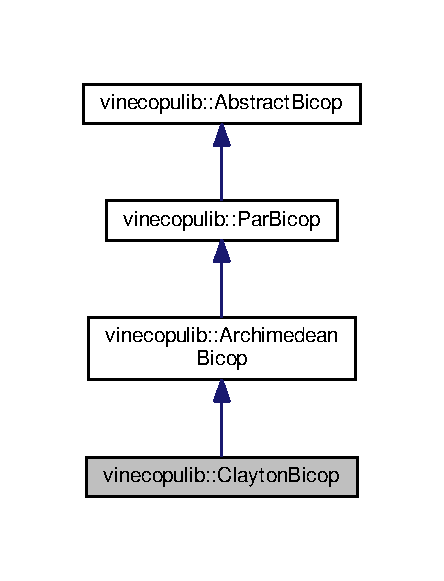
\includegraphics[width=213pt]{classvinecopulib_1_1_clayton_bicop__inherit__graph}
\end{center}
\end{figure}


Collaboration diagram for vinecopulib\+:\+:Clayton\+Bicop\+:\nopagebreak
\begin{figure}[H]
\begin{center}
\leavevmode
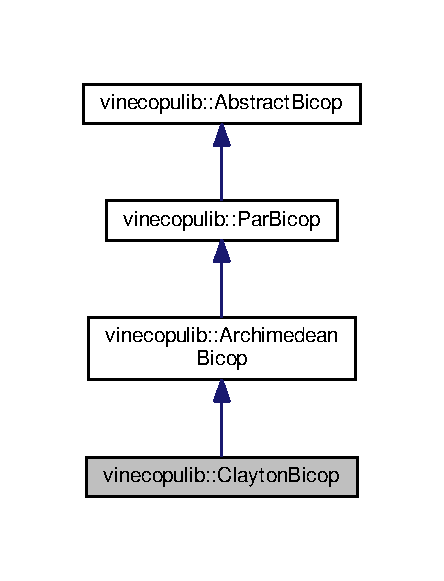
\includegraphics[width=213pt]{classvinecopulib_1_1_clayton_bicop__coll__graph}
\end{center}
\end{figure}
\subsection*{Additional Inherited Members}


\subsection{Detailed Description}
The Clayton copula. 

This class is used in the implementation underlying the \hyperlink{classvinecopulib_1_1_bicop}{Bicop} class. Users should not use \hyperlink{classvinecopulib_1_1_abstract_bicop}{Abstract\+Bicop} or derived classes directly, but always work with the \hyperlink{classvinecopulib_1_1_bicop}{Bicop} interface.

Joe, Harry. Dependence modeling with copulas. C\+RC Press, 2014. 

The documentation for this class was generated from the following files\+:\begin{DoxyCompactItemize}
\item 
/home/n5/dev/cpp/vinecopulib/include/bicop/clayton.\+hpp\item 
/home/n5/dev/cpp/vinecopulib/src/bicop/clayton.\+cpp\end{DoxyCompactItemize}

\hypertarget{classvinecopulib_1_1_elliptical_bicop}{}\section{vinecopulib\+:\+:Elliptical\+Bicop Class Reference}
\label{classvinecopulib_1_1_elliptical_bicop}\index{vinecopulib\+::\+Elliptical\+Bicop@{vinecopulib\+::\+Elliptical\+Bicop}}


An abstract class for elliptical copula families.  




{\ttfamily \#include $<$elliptical.\+hpp$>$}



Inheritance diagram for vinecopulib\+:\+:Elliptical\+Bicop\+:\nopagebreak
\begin{figure}[H]
\begin{center}
\leavevmode
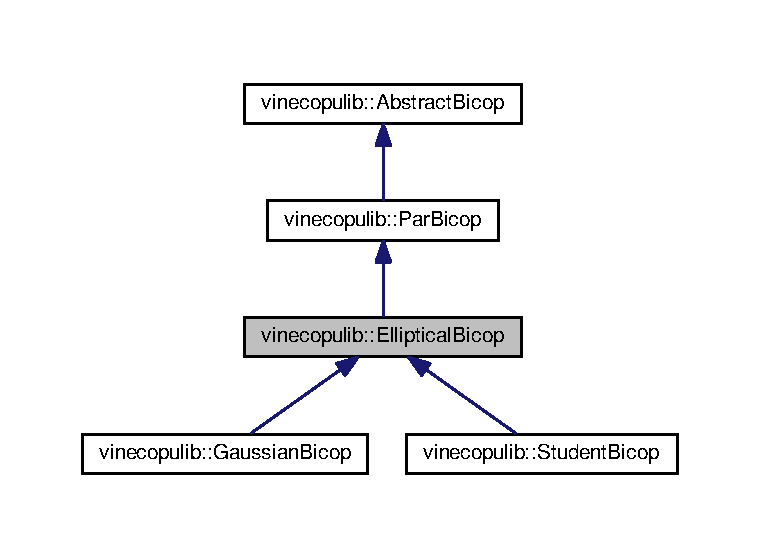
\includegraphics[width=350pt]{classvinecopulib_1_1_elliptical_bicop__inherit__graph}
\end{center}
\end{figure}


Collaboration diagram for vinecopulib\+:\+:Elliptical\+Bicop\+:\nopagebreak
\begin{figure}[H]
\begin{center}
\leavevmode
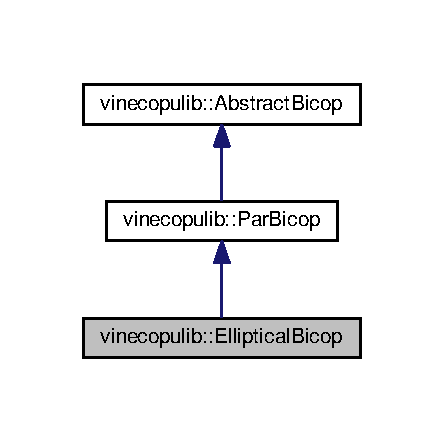
\includegraphics[width=213pt]{classvinecopulib_1_1_elliptical_bicop__coll__graph}
\end{center}
\end{figure}
\subsection*{Additional Inherited Members}


\subsection{Detailed Description}
An abstract class for elliptical copula families. 

This class is used in the implementation underlying the \hyperlink{classvinecopulib_1_1_bicop}{Bicop} class. Users should not use \hyperlink{classvinecopulib_1_1_abstract_bicop}{Abstract\+Bicop} or derived classes directly, but always work with the \hyperlink{classvinecopulib_1_1_bicop}{Bicop} interface.

Joe, Harry. Dependence modeling with copulas. C\+RC Press, 2014. 

The documentation for this class was generated from the following files\+:\begin{DoxyCompactItemize}
\item 
/home/n5/dev/cpp/vinecopulib/include/bicop/elliptical.\+hpp\item 
/home/n5/dev/cpp/vinecopulib/src/bicop/elliptical.\+cpp\end{DoxyCompactItemize}

\hypertarget{classvinecopulib_1_1_frank_bicop}{\section{vinecopulib\+:\+:Frank\+Bicop Class Reference}
\label{classvinecopulib_1_1_frank_bicop}\index{vinecopulib\+::\+Frank\+Bicop@{vinecopulib\+::\+Frank\+Bicop}}
}


The Frank copula.  




{\ttfamily \#include $<$frank.\+hpp$>$}



Inheritance diagram for vinecopulib\+:\+:Frank\+Bicop\+:\nopagebreak
\begin{figure}[H]
\begin{center}
\leavevmode
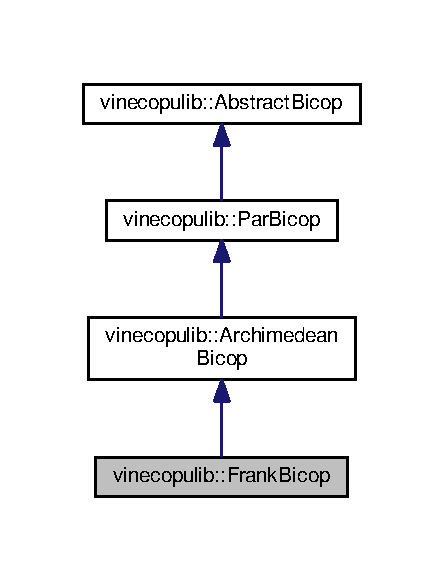
\includegraphics[width=212pt]{classvinecopulib_1_1_frank_bicop__inherit__graph}
\end{center}
\end{figure}


Collaboration diagram for vinecopulib\+:\+:Frank\+Bicop\+:\nopagebreak
\begin{figure}[H]
\begin{center}
\leavevmode
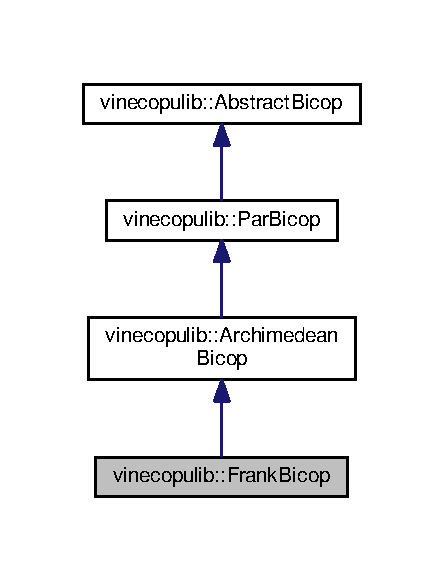
\includegraphics[width=212pt]{classvinecopulib_1_1_frank_bicop__coll__graph}
\end{center}
\end{figure}
\subsection*{Additional Inherited Members}


\subsection{Detailed Description}
The Frank copula. 

This class is used in the implementation underlying the \hyperlink{classvinecopulib_1_1_bicop}{Bicop} class. Users should not use \hyperlink{classvinecopulib_1_1_abstract_bicop}{Abstract\+Bicop} or derived classes directly, but always work with the \hyperlink{classvinecopulib_1_1_bicop}{Bicop} interface.

Joe, Harry. Dependence modeling with copulas. C\+R\+C Press, 2014. 

The documentation for this class was generated from the following files\+:\begin{DoxyCompactItemize}
\item 
vinecopulib/include/vinecopulib/bicop/frank.\+hpp\item 
vinecopulib/src/bicop/frank.\+cpp\end{DoxyCompactItemize}

\hypertarget{classvinecopulib_1_1_gaussian_bicop}{}\section{vinecopulib\+:\+:Gaussian\+Bicop Class Reference}
\label{classvinecopulib_1_1_gaussian_bicop}\index{vinecopulib\+::\+Gaussian\+Bicop@{vinecopulib\+::\+Gaussian\+Bicop}}


The Gaussian copula.  




{\ttfamily \#include $<$gaussian.\+hpp$>$}



Inheritance diagram for vinecopulib\+:\+:Gaussian\+Bicop\+:\nopagebreak
\begin{figure}[H]
\begin{center}
\leavevmode
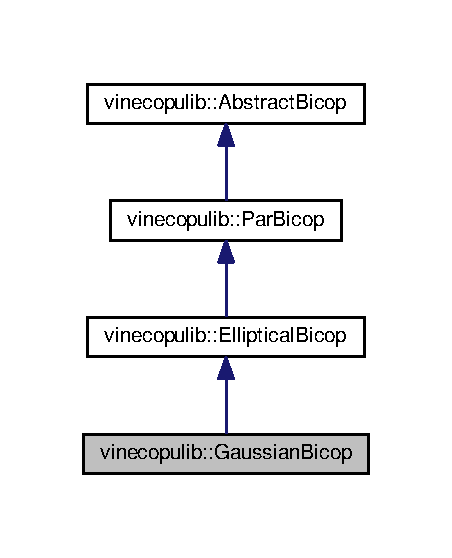
\includegraphics[width=217pt]{classvinecopulib_1_1_gaussian_bicop__inherit__graph}
\end{center}
\end{figure}


Collaboration diagram for vinecopulib\+:\+:Gaussian\+Bicop\+:\nopagebreak
\begin{figure}[H]
\begin{center}
\leavevmode
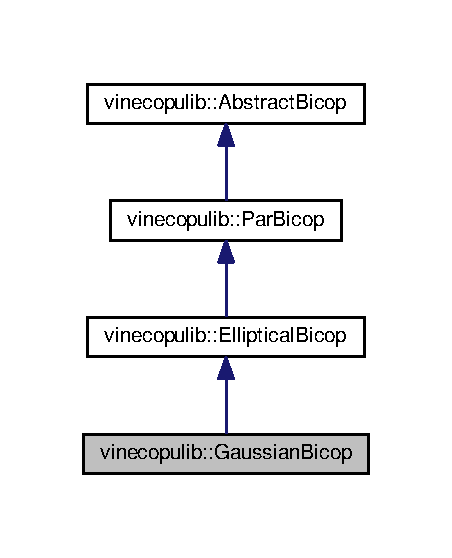
\includegraphics[width=217pt]{classvinecopulib_1_1_gaussian_bicop__coll__graph}
\end{center}
\end{figure}
\subsection*{Additional Inherited Members}


\subsection{Detailed Description}
The Gaussian copula. 

This class is used in the implementation underlying the \hyperlink{classvinecopulib_1_1_bicop}{Bicop} class. Users should not use \hyperlink{classvinecopulib_1_1_abstract_bicop}{Abstract\+Bicop} or derived classes directly, but always work with the \hyperlink{classvinecopulib_1_1_bicop}{Bicop} interface.

Joe, Harry. Dependence modeling with copulas. C\+RC Press, 2014. 

The documentation for this class was generated from the following files\+:\begin{DoxyCompactItemize}
\item 
/home/n5/dev/cpp/vinecopulib/include/bicop/gaussian.\+hpp\item 
/home/n5/dev/cpp/vinecopulib/src/bicop/gaussian.\+cpp\end{DoxyCompactItemize}

\hypertarget{classvinecopulib_1_1_gumbel_bicop}{\section{vinecopulib\+:\+:Gumbel\+Bicop Class Reference}
\label{classvinecopulib_1_1_gumbel_bicop}\index{vinecopulib\+::\+Gumbel\+Bicop@{vinecopulib\+::\+Gumbel\+Bicop}}
}


The Gumbel copula.  




{\ttfamily \#include $<$gumbel.\+hpp$>$}



Inheritance diagram for vinecopulib\+:\+:Gumbel\+Bicop\+:\nopagebreak
\begin{figure}[H]
\begin{center}
\leavevmode
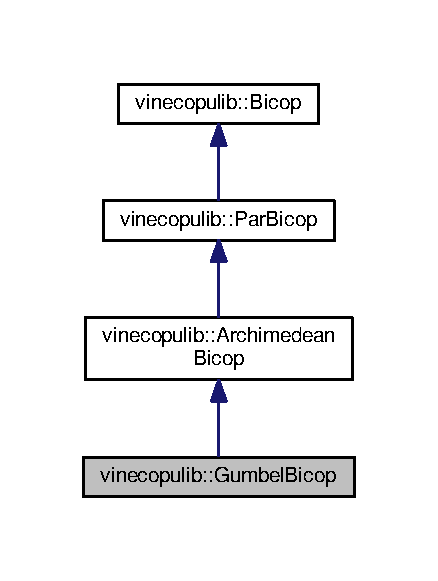
\includegraphics[width=212pt]{classvinecopulib_1_1_gumbel_bicop__inherit__graph}
\end{center}
\end{figure}


Collaboration diagram for vinecopulib\+:\+:Gumbel\+Bicop\+:\nopagebreak
\begin{figure}[H]
\begin{center}
\leavevmode
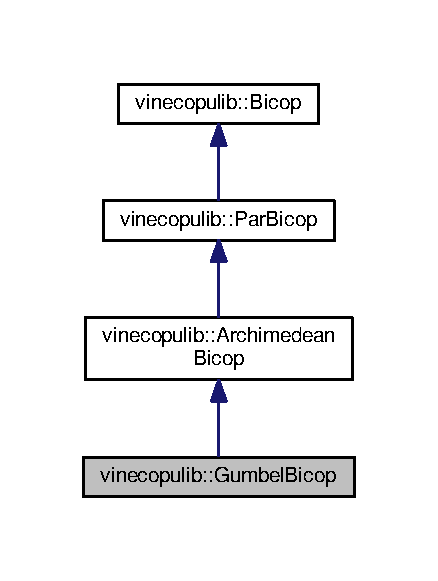
\includegraphics[width=212pt]{classvinecopulib_1_1_gumbel_bicop__coll__graph}
\end{center}
\end{figure}
\subsection*{Additional Inherited Members}


\subsection{Detailed Description}
The Gumbel copula. 

This class is used in the implementation underlying the \hyperlink{classvinecopulib_1_1_bicop}{Bicop} class. Users should not use \hyperlink{classvinecopulib_1_1_abstract_bicop}{Abstract\+Bicop} or derived classes directly, but always work with the \hyperlink{classvinecopulib_1_1_bicop}{Bicop} interface.

Joe, Harry. Dependence modeling with copulas. C\+R\+C Press, 2014. 

The documentation for this class was generated from the following files\+:\begin{DoxyCompactItemize}
\item 
vinecopulib/include/vinecopulib/bicop/gumbel.\+hpp\item 
vinecopulib/src/bicop/gumbel.\+cpp\end{DoxyCompactItemize}

\hypertarget{classvinecopulib_1_1_indep_bicop}{\section{vinecopulib\+:\+:Indep\+Bicop Class Reference}
\label{classvinecopulib_1_1_indep_bicop}\index{vinecopulib\+::\+Indep\+Bicop@{vinecopulib\+::\+Indep\+Bicop}}
}


The independence copula.  




{\ttfamily \#include $<$indep.\+hpp$>$}



Inheritance diagram for vinecopulib\+:\+:Indep\+Bicop\+:\nopagebreak
\begin{figure}[H]
\begin{center}
\leavevmode
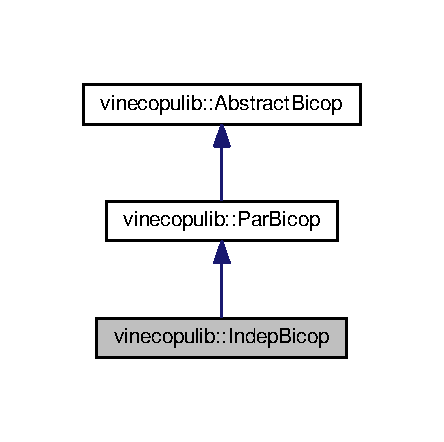
\includegraphics[width=212pt]{classvinecopulib_1_1_indep_bicop__inherit__graph}
\end{center}
\end{figure}


Collaboration diagram for vinecopulib\+:\+:Indep\+Bicop\+:\nopagebreak
\begin{figure}[H]
\begin{center}
\leavevmode
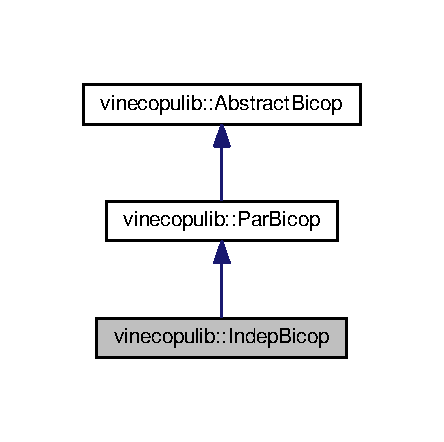
\includegraphics[width=212pt]{classvinecopulib_1_1_indep_bicop__coll__graph}
\end{center}
\end{figure}
\subsection*{Additional Inherited Members}


\subsection{Detailed Description}
The independence copula. 

This class is used in the implementation underlying the \hyperlink{classvinecopulib_1_1_bicop}{Bicop} class. Users should not use \hyperlink{classvinecopulib_1_1_abstract_bicop}{Abstract\+Bicop} or derived classes directly, but always work with the \hyperlink{classvinecopulib_1_1_bicop}{Bicop} interface.

Joe, Harry. Dependence modeling with copulas. C\+R\+C Press, 2014. 

The documentation for this class was generated from the following files\+:\begin{DoxyCompactItemize}
\item 
vinecopulib/include/vinecopulib/bicop/indep.\+hpp\item 
vinecopulib/src/bicop/indep.\+cpp\end{DoxyCompactItemize}

\hypertarget{classvinecopulib_1_1_interpolation_grid}{}\section{vinecopulib\+:\+:Interpolation\+Grid Class Reference}
\label{classvinecopulib_1_1_interpolation_grid}\index{vinecopulib\+::\+Interpolation\+Grid@{vinecopulib\+::\+Interpolation\+Grid}}


{\ttfamily \#include $<$interpolation\+\_\+grid.\+hpp$>$}

\subsection*{Public Member Functions}
\begin{DoxyCompactItemize}
\item 
\hyperlink{classvinecopulib_1_1_interpolation_grid_a9e63e4af3a252454eeae6df38fd8e0ca}{Interpolation\+Grid} (const Eigen\+::\+Vector\+Xd \&grid\+\_\+points, const Eigen\+::\+Matrix\+Xd \&values)
\item 
void {\bfseries flip} ()\hypertarget{classvinecopulib_1_1_interpolation_grid_a8dc18717a2e8dfe5b157571805a25dab}{}\label{classvinecopulib_1_1_interpolation_grid_a8dc18717a2e8dfe5b157571805a25dab}

\item 
Eigen\+::\+Vector\+Xd \hyperlink{classvinecopulib_1_1_interpolation_grid_a7fe207d7f864d2b05654c5efb5e27f35}{interpolate} (const Eigen\+::\+Matrix\+Xd \&x)
\item 
Eigen\+::\+Vector\+Xd \hyperlink{classvinecopulib_1_1_interpolation_grid_aa1811201ba71d8c3375b8e42df6f673a}{intergrate\+\_\+1d} (const Eigen\+::\+Matrix\+Xd \&u, const int \&cond\+\_\+var)
\item 
Eigen\+::\+Vector\+Xd \hyperlink{classvinecopulib_1_1_interpolation_grid_a087c7e9b9c6087b6cbbb8ba7b7292582}{inv\+\_\+intergrate\+\_\+1d} (const Eigen\+::\+Matrix\+Xd \&u, const int \&cond\+\_\+var)
\end{DoxyCompactItemize}


\subsection{Detailed Description}
A class for cubic spline interpolation of bivariate copulas

The class is used for implementing kernel estimators. It makes storing the observations obsolete and allows for fast numerical integration. 

\subsection{Constructor \& Destructor Documentation}
\index{vinecopulib\+::\+Interpolation\+Grid@{vinecopulib\+::\+Interpolation\+Grid}!Interpolation\+Grid@{Interpolation\+Grid}}
\index{Interpolation\+Grid@{Interpolation\+Grid}!vinecopulib\+::\+Interpolation\+Grid@{vinecopulib\+::\+Interpolation\+Grid}}
\subsubsection[{\texorpdfstring{Interpolation\+Grid(const Eigen\+::\+Vector\+Xd \&grid\+\_\+points, const Eigen\+::\+Matrix\+Xd \&values)}{InterpolationGrid(const Eigen::VectorXd &grid_points, const Eigen::MatrixXd &values)}}]{\setlength{\rightskip}{0pt plus 5cm}vinecopulib\+::\+Interpolation\+Grid\+::\+Interpolation\+Grid (
\begin{DoxyParamCaption}
\item[{const Eigen\+::\+Vector\+Xd \&}]{grid\+\_\+points, }
\item[{const Eigen\+::\+Matrix\+Xd \&}]{values}
\end{DoxyParamCaption}
)}\hypertarget{classvinecopulib_1_1_interpolation_grid_a9e63e4af3a252454eeae6df38fd8e0ca}{}\label{classvinecopulib_1_1_interpolation_grid_a9e63e4af3a252454eeae6df38fd8e0ca}
Constructor


\begin{DoxyParams}{Parameters}
{\em grid\+\_\+points} & an ascending sequence of grid\+\_\+points; used in both dimensions. \\
\hline
{\em values} & a dxd matrix of copula density values evaluated at (grid\+\_\+points\+\_\+i, grid\+\_\+points\+\_\+j). \\
\hline
\end{DoxyParams}


\subsection{Member Function Documentation}
\index{vinecopulib\+::\+Interpolation\+Grid@{vinecopulib\+::\+Interpolation\+Grid}!intergrate\+\_\+1d@{intergrate\+\_\+1d}}
\index{intergrate\+\_\+1d@{intergrate\+\_\+1d}!vinecopulib\+::\+Interpolation\+Grid@{vinecopulib\+::\+Interpolation\+Grid}}
\subsubsection[{\texorpdfstring{intergrate\+\_\+1d(const Eigen\+::\+Matrix\+Xd \&u, const int \&cond\+\_\+var)}{intergrate_1d(const Eigen::MatrixXd &u, const int &cond_var)}}]{\setlength{\rightskip}{0pt plus 5cm}Eigen\+::\+Vector\+Xd vinecopulib\+::\+Interpolation\+Grid\+::intergrate\+\_\+1d (
\begin{DoxyParamCaption}
\item[{const Eigen\+::\+Matrix\+Xd \&}]{u, }
\item[{const int \&}]{cond\+\_\+var}
\end{DoxyParamCaption}
)}\hypertarget{classvinecopulib_1_1_interpolation_grid_aa1811201ba71d8c3375b8e42df6f673a}{}\label{classvinecopulib_1_1_interpolation_grid_aa1811201ba71d8c3375b8e42df6f673a}
Integrate the grid along one axis


\begin{DoxyParams}{Parameters}
{\em u} & mx2 matrix of evaluation points \\
\hline
{\em cond\+\_\+var} & either 1 or 2; the axis considered fixed. \\
\hline
\end{DoxyParams}
\index{vinecopulib\+::\+Interpolation\+Grid@{vinecopulib\+::\+Interpolation\+Grid}!interpolate@{interpolate}}
\index{interpolate@{interpolate}!vinecopulib\+::\+Interpolation\+Grid@{vinecopulib\+::\+Interpolation\+Grid}}
\subsubsection[{\texorpdfstring{interpolate(const Eigen\+::\+Matrix\+Xd \&x)}{interpolate(const Eigen::MatrixXd &x)}}]{\setlength{\rightskip}{0pt plus 5cm}Eigen\+::\+Vector\+Xd vinecopulib\+::\+Interpolation\+Grid\+::interpolate (
\begin{DoxyParamCaption}
\item[{const Eigen\+::\+Matrix\+Xd \&}]{x}
\end{DoxyParamCaption}
)}\hypertarget{classvinecopulib_1_1_interpolation_grid_a7fe207d7f864d2b05654c5efb5e27f35}{}\label{classvinecopulib_1_1_interpolation_grid_a7fe207d7f864d2b05654c5efb5e27f35}
Interpolation in two dimensions


\begin{DoxyParams}{Parameters}
{\em x} & mx2 matrix of evaluation points. \\
\hline
\end{DoxyParams}
\index{vinecopulib\+::\+Interpolation\+Grid@{vinecopulib\+::\+Interpolation\+Grid}!inv\+\_\+intergrate\+\_\+1d@{inv\+\_\+intergrate\+\_\+1d}}
\index{inv\+\_\+intergrate\+\_\+1d@{inv\+\_\+intergrate\+\_\+1d}!vinecopulib\+::\+Interpolation\+Grid@{vinecopulib\+::\+Interpolation\+Grid}}
\subsubsection[{\texorpdfstring{inv\+\_\+intergrate\+\_\+1d(const Eigen\+::\+Matrix\+Xd \&u, const int \&cond\+\_\+var)}{inv_intergrate_1d(const Eigen::MatrixXd &u, const int &cond_var)}}]{\setlength{\rightskip}{0pt plus 5cm}Eigen\+::\+Vector\+Xd vinecopulib\+::\+Interpolation\+Grid\+::inv\+\_\+intergrate\+\_\+1d (
\begin{DoxyParamCaption}
\item[{const Eigen\+::\+Matrix\+Xd \&}]{u, }
\item[{const int \&}]{cond\+\_\+var}
\end{DoxyParamCaption}
)}\hypertarget{classvinecopulib_1_1_interpolation_grid_a087c7e9b9c6087b6cbbb8ba7b7292582}{}\label{classvinecopulib_1_1_interpolation_grid_a087c7e9b9c6087b6cbbb8ba7b7292582}
Inverse of integral along one axis of the grid


\begin{DoxyParams}{Parameters}
{\em u} & mx2 matrix of evaluation points \\
\hline
{\em cond\+\_\+var} & either 1 or 2; the axis considered fixed. \\
\hline
\end{DoxyParams}


The documentation for this class was generated from the following files\+:\begin{DoxyCompactItemize}
\item 
/home/n5/dev/cpp/vinecopulib/include/misc/interpolation\+\_\+grid.\+hpp\item 
/home/n5/dev/cpp/vinecopulib/src/misc/interpolation\+\_\+grid.\+cpp\end{DoxyCompactItemize}

\hypertarget{classvinecopulib_1_1_joe_bicop}{}\section{vinecopulib\+:\+:Joe\+Bicop Class Reference}
\label{classvinecopulib_1_1_joe_bicop}\index{vinecopulib\+::\+Joe\+Bicop@{vinecopulib\+::\+Joe\+Bicop}}


The Joe copula.  




{\ttfamily \#include $<$joe.\+hpp$>$}



Inheritance diagram for vinecopulib\+:\+:Joe\+Bicop\+:\nopagebreak
\begin{figure}[H]
\begin{center}
\leavevmode
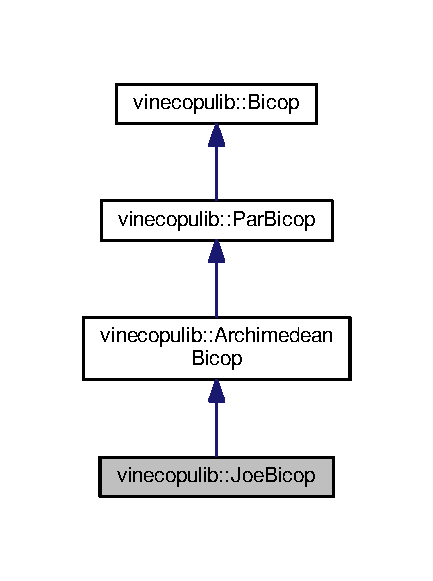
\includegraphics[width=213pt]{classvinecopulib_1_1_joe_bicop__inherit__graph}
\end{center}
\end{figure}


Collaboration diagram for vinecopulib\+:\+:Joe\+Bicop\+:\nopagebreak
\begin{figure}[H]
\begin{center}
\leavevmode
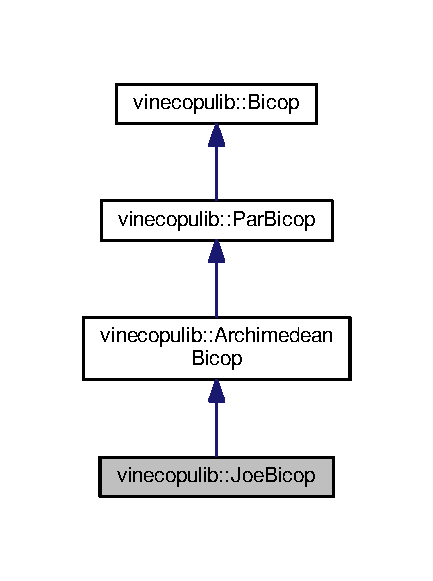
\includegraphics[width=213pt]{classvinecopulib_1_1_joe_bicop__coll__graph}
\end{center}
\end{figure}
\subsection*{Additional Inherited Members}


\subsection{Detailed Description}
The Joe copula. 

This class is used in the implementation underlying the \hyperlink{classvinecopulib_1_1_bicop}{Bicop} class. Users should not use \hyperlink{classvinecopulib_1_1_abstract_bicop}{Abstract\+Bicop} or derived classes directly, but always work with the \hyperlink{classvinecopulib_1_1_bicop}{Bicop} interface.

Joe, Harry. Dependence modeling with copulas. C\+RC Press, 2014. 

The documentation for this class was generated from the following files\+:\begin{DoxyCompactItemize}
\item 
/home/n5/dev/cpp/vinecopulib/include/vinecopulib/bicop/joe.\+hpp\item 
/home/n5/dev/cpp/vinecopulib/src/bicop/joe.\+cpp\end{DoxyCompactItemize}

\hypertarget{classvinecopulib_1_1_kernel_bicop}{}\section{vinecopulib\+:\+:Kernel\+Bicop Class Reference}
\label{classvinecopulib_1_1_kernel_bicop}\index{vinecopulib\+::\+Kernel\+Bicop@{vinecopulib\+::\+Kernel\+Bicop}}


Inheritance diagram for vinecopulib\+:\+:Kernel\+Bicop\+:\nopagebreak
\begin{figure}[H]
\begin{center}
\leavevmode
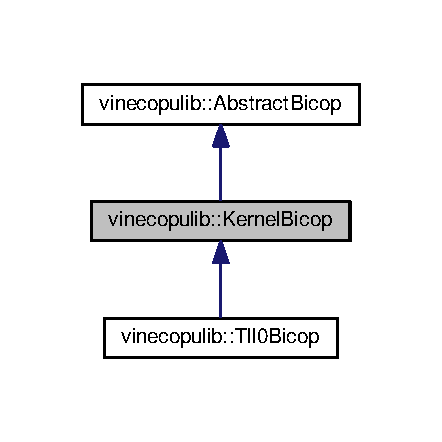
\includegraphics[width=213pt]{classvinecopulib_1_1_kernel_bicop__inherit__graph}
\end{center}
\end{figure}


Collaboration diagram for vinecopulib\+:\+:Kernel\+Bicop\+:\nopagebreak
\begin{figure}[H]
\begin{center}
\leavevmode
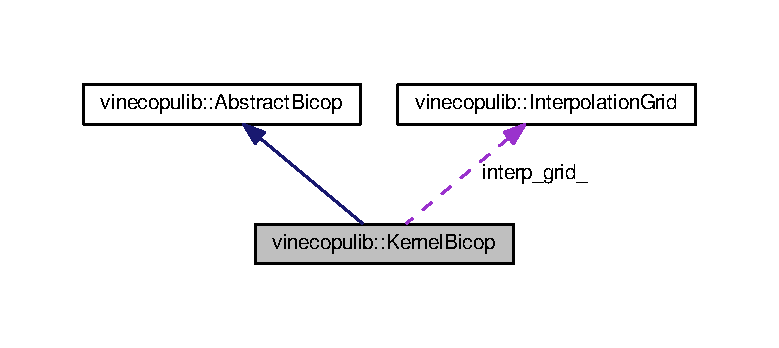
\includegraphics[width=350pt]{classvinecopulib_1_1_kernel_bicop__coll__graph}
\end{center}
\end{figure}
\subsection*{Protected Member Functions}
\begin{DoxyCompactItemize}
\item 
Eigen\+::\+Vector\+Xd {\bfseries pdf} (const Eigen\+::\+Matrix$<$ double, Eigen\+::\+Dynamic, 2 $>$ \&u)\hypertarget{classvinecopulib_1_1_kernel_bicop_a307624ad91ab1fd38ae7933fab0a5f6a}{}\label{classvinecopulib_1_1_kernel_bicop_a307624ad91ab1fd38ae7933fab0a5f6a}

\item 
Eigen\+::\+Vector\+Xd {\bfseries hfunc1} (const Eigen\+::\+Matrix$<$ double, Eigen\+::\+Dynamic, 2 $>$ \&u)\hypertarget{classvinecopulib_1_1_kernel_bicop_a08a6961d233bc977e583b5253c6089dc}{}\label{classvinecopulib_1_1_kernel_bicop_a08a6961d233bc977e583b5253c6089dc}

\item 
Eigen\+::\+Vector\+Xd {\bfseries hfunc2} (const Eigen\+::\+Matrix$<$ double, Eigen\+::\+Dynamic, 2 $>$ \&u)\hypertarget{classvinecopulib_1_1_kernel_bicop_ae4983795f404cca9c4a6af15d41b104a}{}\label{classvinecopulib_1_1_kernel_bicop_ae4983795f404cca9c4a6af15d41b104a}

\item 
Eigen\+::\+Vector\+Xd {\bfseries hinv1} (const Eigen\+::\+Matrix$<$ double, Eigen\+::\+Dynamic, 2 $>$ \&u)\hypertarget{classvinecopulib_1_1_kernel_bicop_aca726ccdf9a1551fb342dd7e60de1f84}{}\label{classvinecopulib_1_1_kernel_bicop_aca726ccdf9a1551fb342dd7e60de1f84}

\item 
Eigen\+::\+Vector\+Xd {\bfseries hinv2} (const Eigen\+::\+Matrix$<$ double, Eigen\+::\+Dynamic, 2 $>$ \&u)\hypertarget{classvinecopulib_1_1_kernel_bicop_a809dc2c7f0a67d217e0fe9651a625a6b}{}\label{classvinecopulib_1_1_kernel_bicop_a809dc2c7f0a67d217e0fe9651a625a6b}

\item 
double {\bfseries parameters\+\_\+to\+\_\+tau} (const Eigen\+::\+Vector\+Xd \&)\hypertarget{classvinecopulib_1_1_kernel_bicop_a1c00a74e12159b2c06487cf1b3ccff00}{}\label{classvinecopulib_1_1_kernel_bicop_a1c00a74e12159b2c06487cf1b3ccff00}

\item 
Eigen\+::\+Matrix\+Xd {\bfseries tau\+\_\+to\+\_\+parameters} (const double \&tau)\hypertarget{classvinecopulib_1_1_kernel_bicop_a510489f8f985c04c4f692e12ab2d1bf0}{}\label{classvinecopulib_1_1_kernel_bicop_a510489f8f985c04c4f692e12ab2d1bf0}

\item 
double {\bfseries calculate\+\_\+npars} ()\hypertarget{classvinecopulib_1_1_kernel_bicop_a33f736d5f443399f1f4dbe54b386aba3}{}\label{classvinecopulib_1_1_kernel_bicop_a33f736d5f443399f1f4dbe54b386aba3}

\item 
void {\bfseries flip} ()\hypertarget{classvinecopulib_1_1_kernel_bicop_abc23a81271f970b9c99dd6ed727c170f}{}\label{classvinecopulib_1_1_kernel_bicop_abc23a81271f970b9c99dd6ed727c170f}

\end{DoxyCompactItemize}
\subsection*{Protected Attributes}
\begin{DoxyCompactItemize}
\item 
\hyperlink{classvinecopulib_1_1_interpolation_grid}{Interpolation\+Grid} {\bfseries interp\+\_\+grid\+\_\+}\hypertarget{classvinecopulib_1_1_kernel_bicop_aa8cfe1dd0786d692562252de05c46588}{}\label{classvinecopulib_1_1_kernel_bicop_aa8cfe1dd0786d692562252de05c46588}

\item 
double {\bfseries npars\+\_\+}\hypertarget{classvinecopulib_1_1_kernel_bicop_a1b49a0a2630e71079c08ebdca79b06b6}{}\label{classvinecopulib_1_1_kernel_bicop_a1b49a0a2630e71079c08ebdca79b06b6}

\end{DoxyCompactItemize}
\subsection*{Additional Inherited Members}


The documentation for this class was generated from the following files\+:\begin{DoxyCompactItemize}
\item 
/home/n5/dev/cpp/vinecopulib/include/bicop/kernel.\+hpp\item 
/home/n5/dev/cpp/vinecopulib/src/bicop/kernel.\+cpp\end{DoxyCompactItemize}

\hypertarget{classvinecopulib_1_1_par_bicop}{}\section{vinecopulib\+:\+:Par\+Bicop Class Reference}
\label{classvinecopulib_1_1_par_bicop}\index{vinecopulib\+::\+Par\+Bicop@{vinecopulib\+::\+Par\+Bicop}}


Inheritance diagram for vinecopulib\+:\+:Par\+Bicop\+:\nopagebreak
\begin{figure}[H]
\begin{center}
\leavevmode
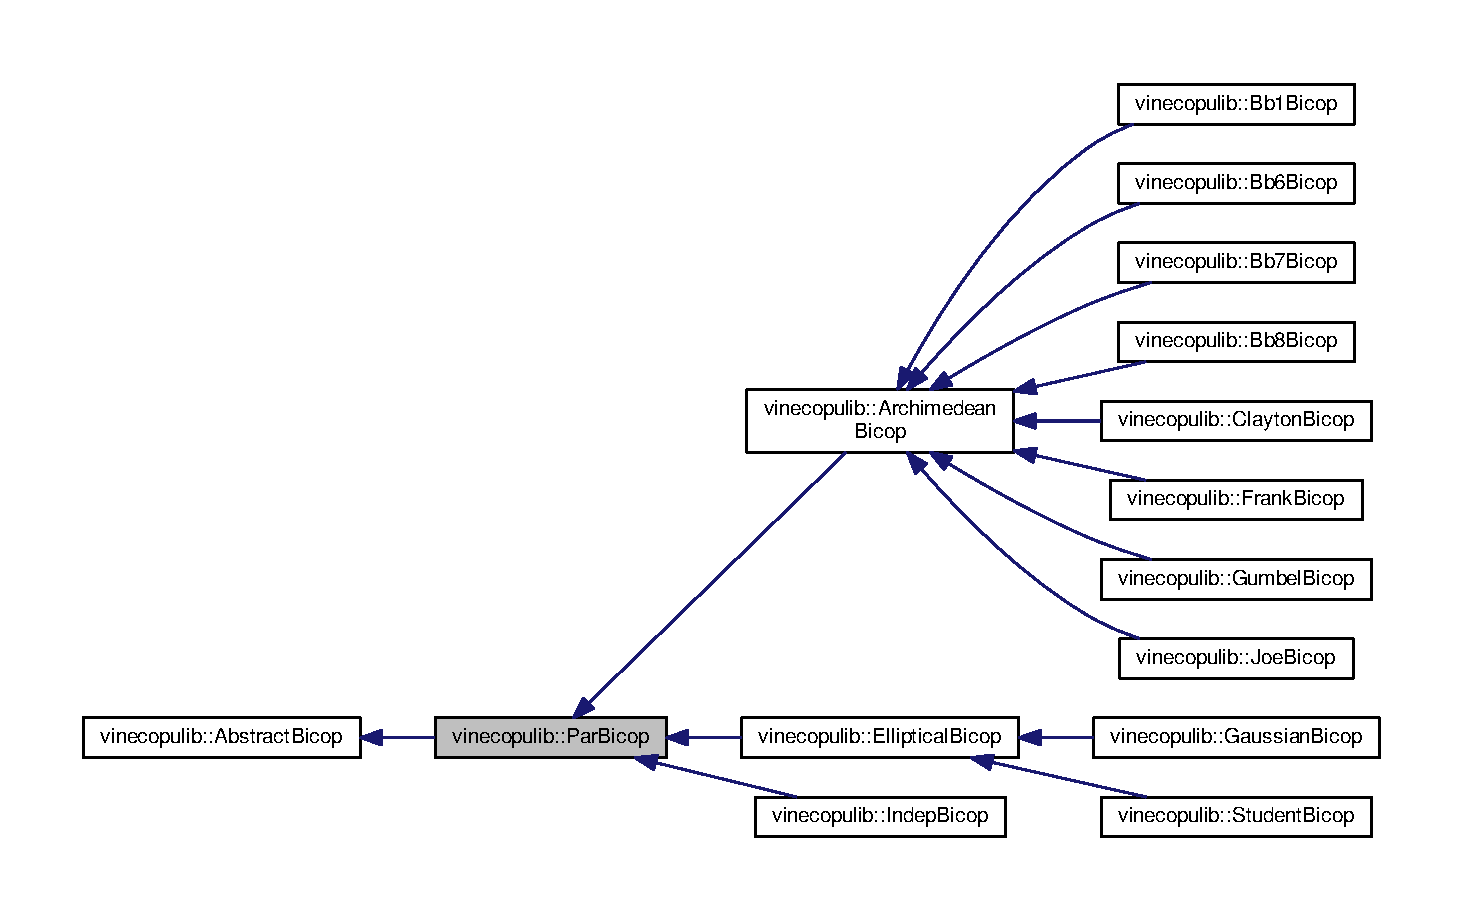
\includegraphics[width=350pt]{classvinecopulib_1_1_par_bicop__inherit__graph}
\end{center}
\end{figure}


Collaboration diagram for vinecopulib\+:\+:Par\+Bicop\+:\nopagebreak
\begin{figure}[H]
\begin{center}
\leavevmode
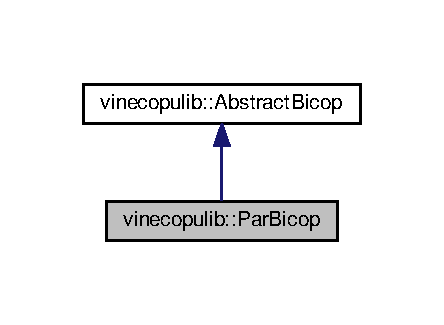
\includegraphics[width=213pt]{classvinecopulib_1_1_par_bicop__coll__graph}
\end{center}
\end{figure}
\subsection*{Additional Inherited Members}


The documentation for this class was generated from the following files\+:\begin{DoxyCompactItemize}
\item 
/home/n5/dev/cpp/vinecopulib/include/bicop/parametric.\+hpp\item 
/home/n5/dev/cpp/vinecopulib/src/bicop/parametric.\+cpp\end{DoxyCompactItemize}

\hypertarget{classvinecopulib_1_1_r_vine_matrix}{}\section{vinecopulib\+:\+:R\+Vine\+Matrix Class Reference}
\label{classvinecopulib_1_1_r_vine_matrix}\index{vinecopulib\+::\+R\+Vine\+Matrix@{vinecopulib\+::\+R\+Vine\+Matrix}}


A class for regular vine matrices.  




{\ttfamily \#include $<$rvine\+\_\+matrix.\+hpp$>$}

\subsection*{Public Member Functions}
\begin{DoxyCompactItemize}
\item 
\hyperlink{classvinecopulib_1_1_r_vine_matrix_a966316e211937ae11e840ef7540a492f}{R\+Vine\+Matrix} (const Eigen\+::\+Matrix$<$ size\+\_\+t, Eigen\+::\+Dynamic, Eigen\+::\+Dynamic $>$ \&matrix, bool check=true)
\item 
size\+\_\+t \hyperlink{classvinecopulib_1_1_r_vine_matrix_a873a94d9065ec4e70f43245c5841741b}{get\+\_\+element} (size\+\_\+t row, size\+\_\+t col) const 
\item 
Eigen\+::\+Matrix$<$ size\+\_\+t, Eigen\+::\+Dynamic, Eigen\+::\+Dynamic $>$ \hyperlink{classvinecopulib_1_1_r_vine_matrix_a37c79233fca1e56e1535cbb37f8d3177}{get\+\_\+matrix} () const \hypertarget{classvinecopulib_1_1_r_vine_matrix_a37c79233fca1e56e1535cbb37f8d3177}{}\label{classvinecopulib_1_1_r_vine_matrix_a37c79233fca1e56e1535cbb37f8d3177}

\begin{DoxyCompactList}\small\item\em extract the matrix. \end{DoxyCompactList}\item 
Eigen\+::\+Matrix$<$ size\+\_\+t, Eigen\+::\+Dynamic, 1 $>$ \hyperlink{classvinecopulib_1_1_r_vine_matrix_a71554c734c3cbb4c066c1f17fe94a284}{get\+\_\+order} () const \hypertarget{classvinecopulib_1_1_r_vine_matrix_a71554c734c3cbb4c066c1f17fe94a284}{}\label{classvinecopulib_1_1_r_vine_matrix_a71554c734c3cbb4c066c1f17fe94a284}

\begin{DoxyCompactList}\small\item\em extracts the variable order in the R-\/vine. \end{DoxyCompactList}\item 
Eigen\+::\+Matrix$<$ size\+\_\+t, Eigen\+::\+Dynamic, Eigen\+::\+Dynamic $>$ \hyperlink{classvinecopulib_1_1_r_vine_matrix_a4e63d8b01e1d89284ca28192676b8a3f}{in\+\_\+natural\+\_\+order} () const 
\item 
Eigen\+::\+Matrix$<$ size\+\_\+t, Eigen\+::\+Dynamic, Eigen\+::\+Dynamic $>$ \hyperlink{classvinecopulib_1_1_r_vine_matrix_aef8bbe14451d023e1c9c113e3812f574}{get\+\_\+max\+\_\+matrix} () const 
\item 
Matrix\+Xb \hyperlink{classvinecopulib_1_1_r_vine_matrix_a6303fc1f643fdf793c867ca7e08e42bc}{get\+\_\+needed\+\_\+hfunc1} () const 
\item 
Matrix\+Xb \hyperlink{classvinecopulib_1_1_r_vine_matrix_a7ac32cf10a966ba567142e9b36106746}{get\+\_\+needed\+\_\+hfunc2} () const 
\item 
bool \hyperlink{classvinecopulib_1_1_r_vine_matrix_a9ac94374329ca2cfee92ce676c7f1c2a}{belongs\+\_\+to\+\_\+structure} (const std\+::vector$<$ size\+\_\+t $>$ conditioned, const std\+::vector$<$ size\+\_\+t $>$ conditioning)
\end{DoxyCompactItemize}
\subsection*{Static Public Member Functions}
\begin{DoxyCompactItemize}
\item 
static Eigen\+::\+Matrix$<$ size\+\_\+t, Eigen\+::\+Dynamic, Eigen\+::\+Dynamic $>$ \hyperlink{classvinecopulib_1_1_r_vine_matrix_ad523b84e2ea41eba4eb982eb9b39471b}{construct\+\_\+d\+\_\+vine\+\_\+matrix} (const Eigen\+::\+Matrix$<$ size\+\_\+t, Eigen\+::\+Dynamic, 1 $>$ \&order)
\end{DoxyCompactItemize}


\subsection{Detailed Description}
A class for regular vine matrices. 

A regular vine (R-\/vine) matrix encodes the structure of a vine. An examplary matrix is 
\begin{DoxyCode}
1 1 1 1
2 2 2 0
3 3 0 0
4 0 0 0
\end{DoxyCode}
 which encodes the following pair-\/copulas\+: 
\begin{DoxyCode}
| tree | edge | pair-copulas   |
|------|------|----------------|
| 0    | 0    | `(4, 1)`       |
|      | 1    | `(3, 1)`       |
|      | 2    | `(2, 1)`       |
| 1    | 0    | `(4, 2; 1)`    |
|      | 1    | `(3, 2; 1)`    |
| 2    | 0    | `(4, 3; 2, 1)` |
\end{DoxyCode}
 Denoting by {\ttfamily M\mbox{[}i, j\mbox{]}} the matrix entry in row {\ttfamily i} and column {\ttfamily j}, the pair-\/copula index for edge {\ttfamily e} in tree {\ttfamily t} of a {\ttfamily d} dimensional vine is {\ttfamily (M\mbox{[}d -\/ 1 -\/ t, e\mbox{]}, M\mbox{[}t, e\mbox{]}; M\mbox{[}t -\/ 1, e\mbox{]}, ..., M\mbox{[}0, e\mbox{]})}. Less formally,
\begin{DoxyEnumerate}
\item Start with the counter-\/diagonal element of column {\ttfamily e} (first conditioned variable).
\item Jump up to the element in row {\ttfamily t} (second conditioned variable).
\item Gather all entries further up in column {\ttfamily e} (conditioning set).
\end{DoxyEnumerate}

A valid R-\/vine matrix must satisfy several conditions which are checked when {\ttfamily R\+Vine\+Matrix()} is called\+:
\begin{DoxyEnumerate}
\item The lower right triangle must only contain zeros.
\item The upper left triangle can only contain numbers between 1 and d.
\item The antidiagonal must contain the numbers 1, ..., d.
\item The antidiagonal entry of a column must not be contained in any column further to the right.
\item The entries of a column must be contained in all columns to the left.
\item The proximity condition must hold\+: For all t = 1, ..., d -\/ 2 and e = 0, ..., d -\/ t -\/ 1 there must exist an index j $>$ d, such that {\ttfamily (M\mbox{[}t, e\mbox{]}, \{M\mbox{[}0, e\mbox{]}, ..., M\mbox{[}t-\/1, e\mbox{]}\})} equals either {\ttfamily (M\mbox{[}d-\/j-\/1, j\mbox{]}, \{M\mbox{[}0, j\mbox{]}, ..., M\mbox{[}t-\/1, j\mbox{]}\})} or {\ttfamily (M\mbox{[}t-\/1, j\mbox{]}, \{M\mbox{[}d-\/j-\/1, j\mbox{]}, M\mbox{[}0, j\mbox{]}, ..., M\mbox{[}t-\/2, j\mbox{]}\})}.
\end{DoxyEnumerate}

Condition 6 already implies conditions 2-\/5, but is more difficult to check by hand. 

\subsection{Constructor \& Destructor Documentation}
\index{vinecopulib\+::\+R\+Vine\+Matrix@{vinecopulib\+::\+R\+Vine\+Matrix}!R\+Vine\+Matrix@{R\+Vine\+Matrix}}
\index{R\+Vine\+Matrix@{R\+Vine\+Matrix}!vinecopulib\+::\+R\+Vine\+Matrix@{vinecopulib\+::\+R\+Vine\+Matrix}}
\subsubsection[{\texorpdfstring{R\+Vine\+Matrix(const Eigen\+::\+Matrix$<$ size\+\_\+t, Eigen\+::\+Dynamic, Eigen\+::\+Dynamic $>$ \&matrix, bool check=true)}{RVineMatrix(const Eigen::Matrix< size_t, Eigen::Dynamic, Eigen::Dynamic > &matrix, bool check=true)}}]{\setlength{\rightskip}{0pt plus 5cm}vinecopulib\+::\+R\+Vine\+Matrix\+::\+R\+Vine\+Matrix (
\begin{DoxyParamCaption}
\item[{const Eigen\+::\+Matrix$<$ size\+\_\+t, Eigen\+::\+Dynamic, Eigen\+::\+Dynamic $>$ \&}]{matrix, }
\item[{bool}]{check = {\ttfamily true}}
\end{DoxyParamCaption}
)}\hypertarget{classvinecopulib_1_1_r_vine_matrix_a966316e211937ae11e840ef7540a492f}{}\label{classvinecopulib_1_1_r_vine_matrix_a966316e211937ae11e840ef7540a492f}
instantiates an \hyperlink{classvinecopulib_1_1_r_vine_matrix}{R\+Vine\+Matrix} object. 
\begin{DoxyParams}{Parameters}
{\em matrix} & a valid R-\/vine matrix. \\
\hline
{\em check} & whether the matrix shall be checked for validity. \\
\hline
\end{DoxyParams}


\subsection{Member Function Documentation}
\index{vinecopulib\+::\+R\+Vine\+Matrix@{vinecopulib\+::\+R\+Vine\+Matrix}!belongs\+\_\+to\+\_\+structure@{belongs\+\_\+to\+\_\+structure}}
\index{belongs\+\_\+to\+\_\+structure@{belongs\+\_\+to\+\_\+structure}!vinecopulib\+::\+R\+Vine\+Matrix@{vinecopulib\+::\+R\+Vine\+Matrix}}
\subsubsection[{\texorpdfstring{belongs\+\_\+to\+\_\+structure(const std\+::vector$<$ size\+\_\+t $>$ conditioned, const std\+::vector$<$ size\+\_\+t $>$ conditioning)}{belongs_to_structure(const std::vector< size_t > conditioned, const std::vector< size_t > conditioning)}}]{\setlength{\rightskip}{0pt plus 5cm}bool vinecopulib\+::\+R\+Vine\+Matrix\+::belongs\+\_\+to\+\_\+structure (
\begin{DoxyParamCaption}
\item[{const std\+::vector$<$ size\+\_\+t $>$}]{conditioned, }
\item[{const std\+::vector$<$ size\+\_\+t $>$}]{conditioning}
\end{DoxyParamCaption}
)}\hypertarget{classvinecopulib_1_1_r_vine_matrix_a9ac94374329ca2cfee92ce676c7f1c2a}{}\label{classvinecopulib_1_1_r_vine_matrix_a9ac94374329ca2cfee92ce676c7f1c2a}
check whether an edge belong to the implied structure


\begin{DoxyParams}{Parameters}
{\em conditioned} & the conditioned set. \\
\hline
{\em conditioning} & the conditioning set. \\
\hline
\end{DoxyParams}
\index{vinecopulib\+::\+R\+Vine\+Matrix@{vinecopulib\+::\+R\+Vine\+Matrix}!construct\+\_\+d\+\_\+vine\+\_\+matrix@{construct\+\_\+d\+\_\+vine\+\_\+matrix}}
\index{construct\+\_\+d\+\_\+vine\+\_\+matrix@{construct\+\_\+d\+\_\+vine\+\_\+matrix}!vinecopulib\+::\+R\+Vine\+Matrix@{vinecopulib\+::\+R\+Vine\+Matrix}}
\subsubsection[{\texorpdfstring{construct\+\_\+d\+\_\+vine\+\_\+matrix(const Eigen\+::\+Matrix$<$ size\+\_\+t, Eigen\+::\+Dynamic, 1 $>$ \&order)}{construct_d_vine_matrix(const Eigen::Matrix< size_t, Eigen::Dynamic, 1 > &order)}}]{\setlength{\rightskip}{0pt plus 5cm}Eigen\+::\+Matrix$<$ size\+\_\+t, Eigen\+::\+Dynamic, Eigen\+::\+Dynamic $>$ vinecopulib\+::\+R\+Vine\+Matrix\+::construct\+\_\+d\+\_\+vine\+\_\+matrix (
\begin{DoxyParamCaption}
\item[{const Eigen\+::\+Matrix$<$ size\+\_\+t, Eigen\+::\+Dynamic, 1 $>$ \&}]{order}
\end{DoxyParamCaption}
)\hspace{0.3cm}{\ttfamily [static]}}\hypertarget{classvinecopulib_1_1_r_vine_matrix_ad523b84e2ea41eba4eb982eb9b39471b}{}\label{classvinecopulib_1_1_r_vine_matrix_ad523b84e2ea41eba4eb982eb9b39471b}
constructs a D-\/vine matrix.

A D-\/vine is a vine where each tree is a path.


\begin{DoxyParams}{Parameters}
{\em order} & order of the variables. \\
\hline
\end{DoxyParams}
\index{vinecopulib\+::\+R\+Vine\+Matrix@{vinecopulib\+::\+R\+Vine\+Matrix}!get\+\_\+element@{get\+\_\+element}}
\index{get\+\_\+element@{get\+\_\+element}!vinecopulib\+::\+R\+Vine\+Matrix@{vinecopulib\+::\+R\+Vine\+Matrix}}
\subsubsection[{\texorpdfstring{get\+\_\+element(size\+\_\+t row, size\+\_\+t col) const }{get_element(size_t row, size_t col) const }}]{\setlength{\rightskip}{0pt plus 5cm}size\+\_\+t vinecopulib\+::\+R\+Vine\+Matrix\+::get\+\_\+element (
\begin{DoxyParamCaption}
\item[{size\+\_\+t}]{row, }
\item[{size\+\_\+t}]{col}
\end{DoxyParamCaption}
) const}\hypertarget{classvinecopulib_1_1_r_vine_matrix_a873a94d9065ec4e70f43245c5841741b}{}\label{classvinecopulib_1_1_r_vine_matrix_a873a94d9065ec4e70f43245c5841741b}
extract matrix\+\_\+(row, col)


\begin{DoxyParams}{Parameters}
{\em row} & \\
\hline
{\em col} & \\
\hline
\end{DoxyParams}
\begin{DoxyReturn}{Returns}
matrix\+\_\+(row, col) 
\end{DoxyReturn}
\index{vinecopulib\+::\+R\+Vine\+Matrix@{vinecopulib\+::\+R\+Vine\+Matrix}!get\+\_\+max\+\_\+matrix@{get\+\_\+max\+\_\+matrix}}
\index{get\+\_\+max\+\_\+matrix@{get\+\_\+max\+\_\+matrix}!vinecopulib\+::\+R\+Vine\+Matrix@{vinecopulib\+::\+R\+Vine\+Matrix}}
\subsubsection[{\texorpdfstring{get\+\_\+max\+\_\+matrix() const }{get_max_matrix() const }}]{\setlength{\rightskip}{0pt plus 5cm}Eigen\+::\+Matrix$<$ size\+\_\+t, Eigen\+::\+Dynamic, Eigen\+::\+Dynamic $>$ vinecopulib\+::\+R\+Vine\+Matrix\+::get\+\_\+max\+\_\+matrix (
\begin{DoxyParamCaption}
{}
\end{DoxyParamCaption}
) const}\hypertarget{classvinecopulib_1_1_r_vine_matrix_aef8bbe14451d023e1c9c113e3812f574}{}\label{classvinecopulib_1_1_r_vine_matrix_aef8bbe14451d023e1c9c113e3812f574}
extracts the maximum matrix.

The maximum matrix is derived from an R-\/vine matrix by iteratively computing the (elementwise) maximum of a row and the row below (starting from the bottom). It is used in estimation and evaluation algorithms to find the right pseudo observations for an edge. \index{vinecopulib\+::\+R\+Vine\+Matrix@{vinecopulib\+::\+R\+Vine\+Matrix}!get\+\_\+needed\+\_\+hfunc1@{get\+\_\+needed\+\_\+hfunc1}}
\index{get\+\_\+needed\+\_\+hfunc1@{get\+\_\+needed\+\_\+hfunc1}!vinecopulib\+::\+R\+Vine\+Matrix@{vinecopulib\+::\+R\+Vine\+Matrix}}
\subsubsection[{\texorpdfstring{get\+\_\+needed\+\_\+hfunc1() const }{get_needed_hfunc1() const }}]{\setlength{\rightskip}{0pt plus 5cm}Matrix\+Xb vinecopulib\+::\+R\+Vine\+Matrix\+::get\+\_\+needed\+\_\+hfunc1 (
\begin{DoxyParamCaption}
{}
\end{DoxyParamCaption}
) const}\hypertarget{classvinecopulib_1_1_r_vine_matrix_a6303fc1f643fdf793c867ca7e08e42bc}{}\label{classvinecopulib_1_1_r_vine_matrix_a6303fc1f643fdf793c867ca7e08e42bc}
extracts a matrix indicating which of the first h-\/functions are needed (it is usually not necessary to apply both h-\/functions for each pair-\/copula). \index{vinecopulib\+::\+R\+Vine\+Matrix@{vinecopulib\+::\+R\+Vine\+Matrix}!get\+\_\+needed\+\_\+hfunc2@{get\+\_\+needed\+\_\+hfunc2}}
\index{get\+\_\+needed\+\_\+hfunc2@{get\+\_\+needed\+\_\+hfunc2}!vinecopulib\+::\+R\+Vine\+Matrix@{vinecopulib\+::\+R\+Vine\+Matrix}}
\subsubsection[{\texorpdfstring{get\+\_\+needed\+\_\+hfunc2() const }{get_needed_hfunc2() const }}]{\setlength{\rightskip}{0pt plus 5cm}Matrix\+Xb vinecopulib\+::\+R\+Vine\+Matrix\+::get\+\_\+needed\+\_\+hfunc2 (
\begin{DoxyParamCaption}
{}
\end{DoxyParamCaption}
) const}\hypertarget{classvinecopulib_1_1_r_vine_matrix_a7ac32cf10a966ba567142e9b36106746}{}\label{classvinecopulib_1_1_r_vine_matrix_a7ac32cf10a966ba567142e9b36106746}
extracts a matrix indicating which of the second h-\/functions are needed (it is usually not necessary to apply both h-\/functions for each pair-\/copula). \index{vinecopulib\+::\+R\+Vine\+Matrix@{vinecopulib\+::\+R\+Vine\+Matrix}!in\+\_\+natural\+\_\+order@{in\+\_\+natural\+\_\+order}}
\index{in\+\_\+natural\+\_\+order@{in\+\_\+natural\+\_\+order}!vinecopulib\+::\+R\+Vine\+Matrix@{vinecopulib\+::\+R\+Vine\+Matrix}}
\subsubsection[{\texorpdfstring{in\+\_\+natural\+\_\+order() const }{in_natural_order() const }}]{\setlength{\rightskip}{0pt plus 5cm}Eigen\+::\+Matrix$<$ size\+\_\+t, Eigen\+::\+Dynamic, Eigen\+::\+Dynamic $>$ vinecopulib\+::\+R\+Vine\+Matrix\+::in\+\_\+natural\+\_\+order (
\begin{DoxyParamCaption}
{}
\end{DoxyParamCaption}
) const}\hypertarget{classvinecopulib_1_1_r_vine_matrix_a4e63d8b01e1d89284ca28192676b8a3f}{}\label{classvinecopulib_1_1_r_vine_matrix_a4e63d8b01e1d89284ca28192676b8a3f}
extracts the R-\/vine matrix in natural order.

Natural order means that the counter-\/diagonal has entries (d, ..., 1). We convert to natural order by relabeling the variables. Most algorithms for estimation and evaluation assume that the R-\/vine matrix is in natural order. 

The documentation for this class was generated from the following files\+:\begin{DoxyCompactItemize}
\item 
vinecopulib/include/vinecopulib/vinecop/rvine\+\_\+matrix.\+hpp\item 
vinecopulib/src/vinecop/rvine\+\_\+matrix.\+cpp\end{DoxyCompactItemize}

\hypertarget{classvinecopulib_1_1_student_bicop}{}\section{vinecopulib\+:\+:Student\+Bicop Class Reference}
\label{classvinecopulib_1_1_student_bicop}\index{vinecopulib\+::\+Student\+Bicop@{vinecopulib\+::\+Student\+Bicop}}


Inheritance diagram for vinecopulib\+:\+:Student\+Bicop\+:\nopagebreak
\begin{figure}[H]
\begin{center}
\leavevmode
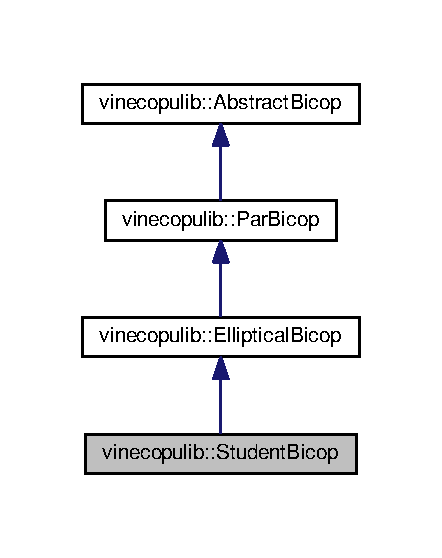
\includegraphics[width=213pt]{classvinecopulib_1_1_student_bicop__inherit__graph}
\end{center}
\end{figure}


Collaboration diagram for vinecopulib\+:\+:Student\+Bicop\+:\nopagebreak
\begin{figure}[H]
\begin{center}
\leavevmode
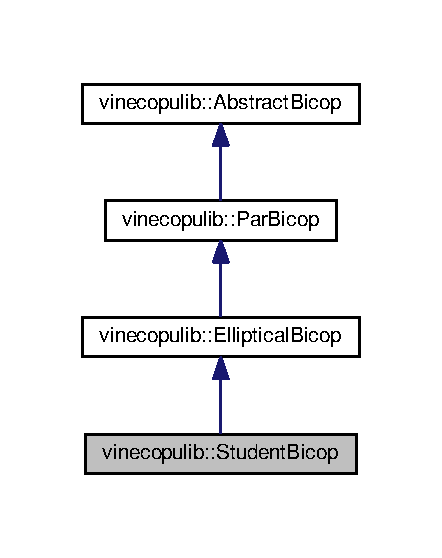
\includegraphics[width=213pt]{classvinecopulib_1_1_student_bicop__coll__graph}
\end{center}
\end{figure}
\subsection*{Additional Inherited Members}


The documentation for this class was generated from the following files\+:\begin{DoxyCompactItemize}
\item 
/home/n5/dev/cpp/vinecopulib/include/bicop\+\_\+student.\+hpp\item 
/home/n5/dev/cpp/vinecopulib/src/bicop\+\_\+student.\+cpp\end{DoxyCompactItemize}

\hypertarget{classvinecopulib_1_1_trafokernel_bicop}{}\section{vinecopulib\+:\+:Trafokernel\+Bicop Class Reference}
\label{classvinecopulib_1_1_trafokernel_bicop}\index{vinecopulib\+::\+Trafokernel\+Bicop@{vinecopulib\+::\+Trafokernel\+Bicop}}


The transformation local-\/constant likelihood estimator.  




{\ttfamily \#include $<$trafokernel.\+hpp$>$}



Inheritance diagram for vinecopulib\+:\+:Trafokernel\+Bicop\+:\nopagebreak
\begin{figure}[H]
\begin{center}
\leavevmode
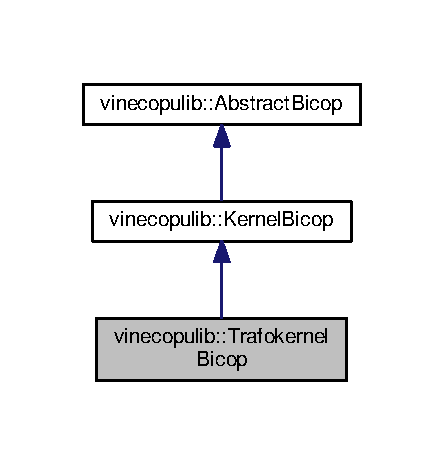
\includegraphics[width=213pt]{classvinecopulib_1_1_trafokernel_bicop__inherit__graph}
\end{center}
\end{figure}


Collaboration diagram for vinecopulib\+:\+:Trafokernel\+Bicop\+:\nopagebreak
\begin{figure}[H]
\begin{center}
\leavevmode
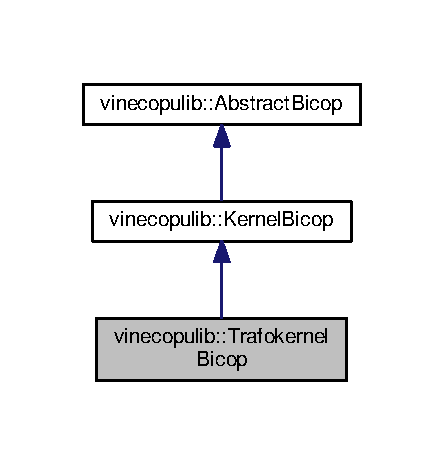
\includegraphics[width=213pt]{classvinecopulib_1_1_trafokernel_bicop__coll__graph}
\end{center}
\end{figure}
\subsection*{Additional Inherited Members}


\subsection{Detailed Description}
The transformation local-\/constant likelihood estimator. 

This class is used in the implementation underlying the \hyperlink{classvinecopulib_1_1_bicop}{Bicop} class. Users should not use \hyperlink{classvinecopulib_1_1_abstract_bicop}{Abstract\+Bicop} or derived classes directly, but always work with the \hyperlink{classvinecopulib_1_1_bicop}{Bicop} interface.

Nagler, Thomas. {\itshape kdecopula\+: An R Package for the Kernel Estimation of Copula Densities}. ar\+Xiv\+:1603.\+04229 \mbox{[}stat.\+CO\mbox{]}, 2016 

The documentation for this class was generated from the following files\+:\begin{DoxyCompactItemize}
\item 
/home/n5/dev/cpp/vinecopulib/include/bicop/trafokernel.\+hpp\item 
/home/n5/dev/cpp/vinecopulib/src/bicop/trafokernel.\+cpp\end{DoxyCompactItemize}

\hypertarget{classvinecopulib_1_1_vinecop}{}\section{vinecopulib\+:\+:Vinecop Class Reference}
\label{classvinecopulib_1_1_vinecop}\index{vinecopulib\+::\+Vinecop@{vinecopulib\+::\+Vinecop}}


A class for vine copula models.  




{\ttfamily \#include $<$class.\+hpp$>$}

\subsection*{Public Member Functions}
\begin{DoxyCompactItemize}
\item 
\hyperlink{classvinecopulib_1_1_vinecop_a391541e2795d06a848d5a17fe3496a63}{Vinecop} (size\+\_\+t d)
\begin{DoxyCompactList}\small\item\em creates a D-\/vine on {\ttfamily d} variables with all pair-\/copulas set to independence. \end{DoxyCompactList}\item 
\hyperlink{classvinecopulib_1_1_vinecop_abebc47fd9c68aeff199a3eba370a5f6a}{Vinecop} (const \hyperlink{classvinecopulib_1_1_r_vine_structure}{R\+Vine\+Structure} \&vine\+\_\+struct)
\begin{DoxyCompactList}\small\item\em creates a vine copula with structure specified by an \hyperlink{classvinecopulib_1_1_r_vine_structure}{R\+Vine\+Structure} object; all pair-\/copulas are set to independence. \end{DoxyCompactList}\item 
\hyperlink{classvinecopulib_1_1_vinecop_a2cb5079a1a3cfe0403969aba92092ac3}{Vinecop} (const Eigen\+::\+Matrix$<$ size\+\_\+t, Eigen\+::\+Dynamic, Eigen\+::\+Dynamic $>$ \&matrix, const bool check\+\_\+matrix=true)
\begin{DoxyCompactList}\small\item\em creates a vine copula with structure specified by an R-\/vine matrix; all pair-\/copulas are set to independence. \end{DoxyCompactList}\item 
\hyperlink{classvinecopulib_1_1_vinecop_af54ae0403aaa188052c63e959e70f90f}{Vinecop} (const std\+::vector$<$ size\+\_\+t $>$ \&order, const \hyperlink{classvinecopulib_1_1_triangular_array}{Triangular\+Array}$<$ size\+\_\+t $>$ \&struct\+\_\+array, const bool check\+\_\+array=true)
\begin{DoxyCompactList}\small\item\em creates a vine copula with structure specified by an R-\/vine matrix; all pair-\/copulas are set to independence. \end{DoxyCompactList}\item 
\hyperlink{classvinecopulib_1_1_vinecop_a6f41f3f14cd479a62bef7448c00376d0}{Vinecop} (const std\+::vector$<$ std\+::vector$<$ \hyperlink{classvinecopulib_1_1_bicop}{Bicop} $>$$>$ \&pair\+\_\+copulas, const \hyperlink{classvinecopulib_1_1_r_vine_structure}{R\+Vine\+Structure} \&vine\+\_\+struct)
\begin{DoxyCompactList}\small\item\em creates an arbitrary vine copula model. \end{DoxyCompactList}\item 
\hyperlink{classvinecopulib_1_1_vinecop_abc94737980ef5dbdc16b7d0aa66e683d}{Vinecop} (const std\+::vector$<$ std\+::vector$<$ \hyperlink{classvinecopulib_1_1_bicop}{Bicop} $>$$>$ \&pair\+\_\+copulas, const Eigen\+::\+Matrix$<$ size\+\_\+t, Eigen\+::\+Dynamic, Eigen\+::\+Dynamic $>$ \&matrix, const bool check\+\_\+matrix=true)
\begin{DoxyCompactList}\small\item\em creates an arbitrary vine copula model. \end{DoxyCompactList}\item 
\hyperlink{classvinecopulib_1_1_vinecop_ae15da62d7cd3829bbd2980fe4ac190b0}{Vinecop} (const std\+::vector$<$ std\+::vector$<$ \hyperlink{classvinecopulib_1_1_bicop}{Bicop} $>$$>$ \&pair\+\_\+copulas, const std\+::vector$<$ size\+\_\+t $>$ \&order, const \hyperlink{classvinecopulib_1_1_triangular_array}{Triangular\+Array}$<$ size\+\_\+t $>$ \&struct\+\_\+array, const bool check\+\_\+array=true)
\begin{DoxyCompactList}\small\item\em creates an arbitrary vine copula model. \end{DoxyCompactList}\item 
\hyperlink{classvinecopulib_1_1_vinecop_a8b389e32ae8d1a2c26046a6be19040f0}{Vinecop} (const Eigen\+::\+Matrix\+Xd \&data, const \hyperlink{classvinecopulib_1_1_fit_controls_vinecop}{Fit\+Controls\+Vinecop} \&controls=\hyperlink{classvinecopulib_1_1_fit_controls_vinecop}{Fit\+Controls\+Vinecop}())
\begin{DoxyCompactList}\small\item\em constructs a vine copula model from data by creating a model and calling \hyperlink{classvinecopulib_1_1_vinecop_a0d2fae568f3d893c1c144a8034fbaf90}{select\+\_\+all()}. \end{DoxyCompactList}\item 
\hyperlink{classvinecopulib_1_1_vinecop_ac8e2119b7cd9d2f67a8a62e7b4fbd61f}{Vinecop} (const Eigen\+::\+Matrix\+Xd \&data, const \hyperlink{classvinecopulib_1_1_r_vine_structure}{R\+Vine\+Structure} \&vine\+\_\+struct, \hyperlink{classvinecopulib_1_1_fit_controls_vinecop}{Fit\+Controls\+Vinecop} controls=\hyperlink{classvinecopulib_1_1_fit_controls_vinecop}{Fit\+Controls\+Vinecop}())
\begin{DoxyCompactList}\small\item\em constructs a vine copula model from data by creating a model and calling select\+\_\+family(). \end{DoxyCompactList}\item 
\hyperlink{classvinecopulib_1_1_vinecop_a228e7c92a06fbf7020870eec625a0e80}{Vinecop} (const Eigen\+::\+Matrix\+Xd \&data, const Eigen\+::\+Matrix$<$ size\+\_\+t, Eigen\+::\+Dynamic, Eigen\+::\+Dynamic $>$ \&matrix, \hyperlink{classvinecopulib_1_1_fit_controls_vinecop}{Fit\+Controls\+Vinecop} controls=\hyperlink{classvinecopulib_1_1_fit_controls_vinecop}{Fit\+Controls\+Vinecop}(), const bool check\+\_\+matrix=true)
\begin{DoxyCompactList}\small\item\em constructs a vine copula model from data by creating a model and calling select\+\_\+family(). \end{DoxyCompactList}\item 
\hyperlink{classvinecopulib_1_1_vinecop_ae91e02b92cd4af43596131cce9b085d9}{Vinecop} (const Eigen\+::\+Matrix\+Xd \&data, const std\+::vector$<$ size\+\_\+t $>$ \&order, const \hyperlink{classvinecopulib_1_1_triangular_array}{Triangular\+Array}$<$ size\+\_\+t $>$ \&struct\+\_\+array, \hyperlink{classvinecopulib_1_1_fit_controls_vinecop}{Fit\+Controls\+Vinecop} controls=\hyperlink{classvinecopulib_1_1_fit_controls_vinecop}{Fit\+Controls\+Vinecop}(), const bool check\+\_\+array=true)
\begin{DoxyCompactList}\small\item\em constructs a vine copula model from data by creating a model and calling select\+\_\+family(). \end{DoxyCompactList}\item 
\hyperlink{classvinecopulib_1_1_vinecop_ac77c6f78b0e2c7860d7406c9ea7fe251}{Vinecop} (const char $\ast$filename, const bool check\+\_\+matrix=true)
\begin{DoxyCompactList}\small\item\em creates from a J\+S\+ON file. \end{DoxyCompactList}\item 
\hyperlink{classvinecopulib_1_1_vinecop_a83e7fdc7c3aef45d8431005b5d1abb83}{Vinecop} (const boost\+::property\+\_\+tree\+::ptree input, const bool check\+\_\+matrix=true)
\begin{DoxyCompactList}\small\item\em creates from a boost\+::property\+\_\+tree\+::ptree object \end{DoxyCompactList}\item 
boost\+::property\+\_\+tree\+::ptree \hyperlink{classvinecopulib_1_1_vinecop_aaee91f92acc8402eb7358b65c8fe63f8}{to\+\_\+ptree} () const
\begin{DoxyCompactList}\small\item\em converts the copula into a boost\+::property\+\_\+tree\+::ptree object. \end{DoxyCompactList}\item 
void \hyperlink{classvinecopulib_1_1_vinecop_acab8a34d8f89da6be0ab6ae77427c09f}{to\+\_\+json} (const char $\ast$filename) const
\begin{DoxyCompactList}\small\item\em write the copula object into a J\+S\+ON file. \end{DoxyCompactList}\item 
void \hyperlink{classvinecopulib_1_1_vinecop_a0d2fae568f3d893c1c144a8034fbaf90}{select\+\_\+all} (const Eigen\+::\+Matrix\+Xd \&data, const \hyperlink{classvinecopulib_1_1_fit_controls_vinecop}{Fit\+Controls\+Vinecop} \&controls=\hyperlink{classvinecopulib_1_1_fit_controls_vinecop}{Fit\+Controls\+Vinecop}())
\begin{DoxyCompactList}\small\item\em automatically fits and selects a vine copula model. \end{DoxyCompactList}\item 
void \hyperlink{classvinecopulib_1_1_vinecop_a5e6cacd0883811fcd80c772ace747c43}{select\+\_\+families} (const Eigen\+::\+Matrix\+Xd \&data, const \hyperlink{classvinecopulib_1_1_fit_controls_vinecop}{Fit\+Controls\+Vinecop} \&controls=\hyperlink{classvinecopulib_1_1_fit_controls_vinecop}{Fit\+Controls\+Vinecop}())
\begin{DoxyCompactList}\small\item\em automatically selects all pair-\/copula families and fits all parameters. \end{DoxyCompactList}\item 
Eigen\+::\+Vector\+Xd \hyperlink{classvinecopulib_1_1_vinecop_ad4ba574fee5f39170e1a38b921a4c02f}{pdf} (const Eigen\+::\+Matrix\+Xd \&u, const size\+\_\+t num\+\_\+threads=1) const
\begin{DoxyCompactList}\small\item\em calculates the density function of the vine copula model. \end{DoxyCompactList}\item 
Eigen\+::\+Vector\+Xd \hyperlink{classvinecopulib_1_1_vinecop_a7db9bc6b406d03e51f2e6e66af0f5ed1}{cdf} (const Eigen\+::\+Matrix\+Xd \&u, const size\+\_\+t N=1e4, const size\+\_\+t num\+\_\+threads=1, std\+::vector$<$ int $>$ seeds=std\+::vector$<$ int $>$()) const
\begin{DoxyCompactList}\small\item\em calculates the cumulative distribution of the vine copula model. \end{DoxyCompactList}\item 
Eigen\+::\+Matrix\+Xd \hyperlink{classvinecopulib_1_1_vinecop_a1221d844d9850435708f21494b80d39f}{simulate} (const size\+\_\+t n, const bool qrng=false, const size\+\_\+t num\+\_\+threads=1, const std\+::vector$<$ int $>$ \&seeds=std\+::vector$<$ int $>$()) const
\begin{DoxyCompactList}\small\item\em simulates from a vine copula model, see \hyperlink{classvinecopulib_1_1_vinecop_a73da79be3f0f3cb892afbd8f41dcad6b}{inverse\+\_\+rosenblatt()}. \end{DoxyCompactList}\item 
Eigen\+::\+Matrix\+Xd \hyperlink{classvinecopulib_1_1_vinecop_a9df88fb9bcdcc420b0771a96943c7d45}{rosenblatt} (const Eigen\+::\+Matrix\+Xd \&u, const size\+\_\+t num\+\_\+threads=1) const
\begin{DoxyCompactList}\small\item\em calculates the Rosenblatt transform for a vine copula model. \end{DoxyCompactList}\item 
Eigen\+::\+Matrix\+Xd \hyperlink{classvinecopulib_1_1_vinecop_a73da79be3f0f3cb892afbd8f41dcad6b}{inverse\+\_\+rosenblatt} (const Eigen\+::\+Matrix\+Xd \&u, const size\+\_\+t num\+\_\+threads=1) const
\begin{DoxyCompactList}\small\item\em calculates the inverse Rosenblatt transform for a vine copula model. \end{DoxyCompactList}\item 
\mbox{\Hypertarget{classvinecopulib_1_1_vinecop_a2b4b1151c5b0a817811628aa59de7eea}\label{classvinecopulib_1_1_vinecop_a2b4b1151c5b0a817811628aa59de7eea}} 
double \hyperlink{classvinecopulib_1_1_vinecop_a2b4b1151c5b0a817811628aa59de7eea}{calculate\+\_\+npars} () const
\begin{DoxyCompactList}\small\item\em returns sum of the number of parameters for all pair copulas (see \hyperlink{classvinecopulib_1_1_bicop_a8e6b3e3dd484d07cafeb24ca3393f5f0}{Bicop\+::calculate\+\_\+npars()}). \end{DoxyCompactList}\item 
double \hyperlink{classvinecopulib_1_1_vinecop_a07e9c59b42d0668df5fc5e69b281272e}{loglik} (const Eigen\+::\+Matrix\+Xd \&u, const size\+\_\+t num\+\_\+threads=1) const
\begin{DoxyCompactList}\small\item\em calculates the log-\/likelihood. \end{DoxyCompactList}\item 
double \hyperlink{classvinecopulib_1_1_vinecop_a082d0c740fcb5610c8d7687cf12a95e4}{aic} (const Eigen\+::\+Matrix\+Xd \&u, const size\+\_\+t num\+\_\+threads=1) const
\begin{DoxyCompactList}\small\item\em calculates the Akaike information criterion (A\+IC). \end{DoxyCompactList}\item 
double \hyperlink{classvinecopulib_1_1_vinecop_a61745ef0b908f6580a5af8fb40221869}{bic} (const Eigen\+::\+Matrix\+Xd \&u, const size\+\_\+t num\+\_\+threads=1) const
\begin{DoxyCompactList}\small\item\em calculates the Bayesian information criterion (B\+IC). \end{DoxyCompactList}\item 
double \hyperlink{classvinecopulib_1_1_vinecop_abb2e75c3531d813125dda78017f0b219}{mbicv} (const Eigen\+::\+Matrix\+Xd \&u, const double psi0, const size\+\_\+t num\+\_\+threads=1) const
\begin{DoxyCompactList}\small\item\em calculates the modified Bayesian information criterion for vines (m\+B\+I\+CV). \end{DoxyCompactList}\item 
void \hyperlink{classvinecopulib_1_1_vinecop_ac77812a69ccd568b7eb0c21658001640}{truncate} (size\+\_\+t trunc\+\_\+lvl)
\begin{DoxyCompactList}\small\item\em truncate the vine copula model. \end{DoxyCompactList}\end{DoxyCompactItemize}
\subsection*{Static Public Member Functions}
\begin{DoxyCompactItemize}
\item 
static std\+::vector$<$ std\+::vector$<$ \hyperlink{classvinecopulib_1_1_bicop}{Bicop} $>$ $>$ \hyperlink{classvinecopulib_1_1_vinecop_ac99ec5154d923ee5eb73fdad071bca46}{make\+\_\+pair\+\_\+copula\+\_\+store} (const size\+\_\+t d, const size\+\_\+t trunc\+\_\+lvl=std\+::numeric\+\_\+limits$<$ size\+\_\+t $>$\+::max())
\begin{DoxyCompactList}\small\item\em initializes object for storing pair copulas. \end{DoxyCompactList}\end{DoxyCompactItemize}
\subsection*{Getters}
\begin{DoxyCompactItemize}
\item 
\hyperlink{classvinecopulib_1_1_bicop}{Bicop} \hyperlink{classvinecopulib_1_1_vinecop_a5a75b825ad6091d734dc163c3277b36b}{get\+\_\+pair\+\_\+copula} (size\+\_\+t tree, size\+\_\+t edge) const
\begin{DoxyCompactList}\small\item\em extracts a pair copula. \end{DoxyCompactList}\item 
\hyperlink{namespacevinecopulib_a42e95cc06d33896199caab0c11ad44f3}{Bicop\+Family} \hyperlink{classvinecopulib_1_1_vinecop_a5c909eae77a38558d46d6d4b98564e57}{get\+\_\+family} (size\+\_\+t tree, size\+\_\+t edge) const
\begin{DoxyCompactList}\small\item\em extracts the family of a pair copula. \end{DoxyCompactList}\item 
int \hyperlink{classvinecopulib_1_1_vinecop_a889a0c1c5c143e32cf34aa9bd15e33b6}{get\+\_\+rotation} (size\+\_\+t tree, size\+\_\+t edge) const
\begin{DoxyCompactList}\small\item\em extracts the rotation of a pair copula. \end{DoxyCompactList}\item 
Eigen\+::\+Matrix\+Xd \hyperlink{classvinecopulib_1_1_vinecop_a16872eaecac2cf3f90c7f282c453fe58}{get\+\_\+parameters} (size\+\_\+t tree, size\+\_\+t edge) const
\begin{DoxyCompactList}\small\item\em extracts the parameters of a pair copula. \end{DoxyCompactList}\item 
double \hyperlink{classvinecopulib_1_1_vinecop_a3f4cc62395a9ae4ce2b7714ceae6bde3}{get\+\_\+tau} (size\+\_\+t tree, size\+\_\+t edge) const
\begin{DoxyCompactList}\small\item\em extracts the Kendall\textquotesingle{}s $ tau $ of a pair copula. \end{DoxyCompactList}\item 
\mbox{\Hypertarget{classvinecopulib_1_1_vinecop_a508971cf99ce5a94712168d10b736812}\label{classvinecopulib_1_1_vinecop_a508971cf99ce5a94712168d10b736812}} 
size\+\_\+t {\bfseries get\+\_\+trunc\+\_\+lvl} () const
\item 
std\+::vector$<$ std\+::vector$<$ \hyperlink{classvinecopulib_1_1_bicop}{Bicop} $>$ $>$ \hyperlink{classvinecopulib_1_1_vinecop_a5f1c76c0fd97ea586b182f7996034e86}{get\+\_\+all\+\_\+pair\+\_\+copulas} () const
\begin{DoxyCompactList}\small\item\em extracts all pair copulas. \end{DoxyCompactList}\item 
std\+::vector$<$ std\+::vector$<$ \hyperlink{namespacevinecopulib_a42e95cc06d33896199caab0c11ad44f3}{Bicop\+Family} $>$ $>$ \hyperlink{classvinecopulib_1_1_vinecop_ab8a6a5d111b80788955438e1630f04c9}{get\+\_\+all\+\_\+families} () const
\begin{DoxyCompactList}\small\item\em extracts the families of all pair copulas. \end{DoxyCompactList}\item 
std\+::vector$<$ std\+::vector$<$ int $>$ $>$ \hyperlink{classvinecopulib_1_1_vinecop_a45dd56984cf7395494ed3fab75c62a1e}{get\+\_\+all\+\_\+rotations} () const
\begin{DoxyCompactList}\small\item\em extracts the rotations of all pair copulas. \end{DoxyCompactList}\item 
std\+::vector$<$ std\+::vector$<$ Eigen\+::\+Matrix\+Xd $>$ $>$ \hyperlink{classvinecopulib_1_1_vinecop_adbd6c2e57666bcec101bc2cc8846c78b}{get\+\_\+all\+\_\+parameters} () const
\begin{DoxyCompactList}\small\item\em extracts the parameters of all pair copulas. \end{DoxyCompactList}\item 
std\+::vector$<$ std\+::vector$<$ double $>$ $>$ \hyperlink{classvinecopulib_1_1_vinecop_ac271e64e1b2dd16f8b5ccaecf3f03e96}{get\+\_\+all\+\_\+taus} () const
\begin{DoxyCompactList}\small\item\em extracts the Kendall\textquotesingle{}s $ tau $s of all pair copulas. \end{DoxyCompactList}\item 
\mbox{\Hypertarget{classvinecopulib_1_1_vinecop_a27e9d72fa28b4d167dde9ae9205ec995}\label{classvinecopulib_1_1_vinecop_a27e9d72fa28b4d167dde9ae9205ec995}} 
size\+\_\+t \hyperlink{classvinecopulib_1_1_vinecop_a27e9d72fa28b4d167dde9ae9205ec995}{get\+\_\+dim} () const
\begin{DoxyCompactList}\small\item\em extracts the dimension of the vine copula model. \end{DoxyCompactList}\item 
\mbox{\Hypertarget{classvinecopulib_1_1_vinecop_a4aff71e7b65688ff04205ec66b34473e}\label{classvinecopulib_1_1_vinecop_a4aff71e7b65688ff04205ec66b34473e}} 
std\+::vector$<$ size\+\_\+t $>$ \hyperlink{classvinecopulib_1_1_vinecop_a4aff71e7b65688ff04205ec66b34473e}{get\+\_\+order} () const
\begin{DoxyCompactList}\small\item\em extracts the order vector of the vine copula model. \end{DoxyCompactList}\item 
\mbox{\Hypertarget{classvinecopulib_1_1_vinecop_aeaaad4d204e86a0df21becfa26032e47}\label{classvinecopulib_1_1_vinecop_aeaaad4d204e86a0df21becfa26032e47}} 
\hyperlink{classvinecopulib_1_1_r_vine_structure}{R\+Vine\+Structure} \hyperlink{classvinecopulib_1_1_vinecop_aeaaad4d204e86a0df21becfa26032e47}{get\+\_\+rvine\+\_\+structure} () const
\begin{DoxyCompactList}\small\item\em extracts the structure matrix of the vine copula model. \end{DoxyCompactList}\item 
\mbox{\Hypertarget{classvinecopulib_1_1_vinecop_aab1af57bb6b7e02029dcc3dc2a285314}\label{classvinecopulib_1_1_vinecop_aab1af57bb6b7e02029dcc3dc2a285314}} 
Eigen\+::\+Matrix$<$ size\+\_\+t, Eigen\+::\+Dynamic, Eigen\+::\+Dynamic $>$ \hyperlink{classvinecopulib_1_1_vinecop_aab1af57bb6b7e02029dcc3dc2a285314}{get\+\_\+matrix} () const
\begin{DoxyCompactList}\small\item\em extracts the structure matrix of the vine copula model. \end{DoxyCompactList}\item 
\mbox{\Hypertarget{classvinecopulib_1_1_vinecop_a4d0f5a7e4b60e6d58aef3020577aeb5a}\label{classvinecopulib_1_1_vinecop_a4d0f5a7e4b60e6d58aef3020577aeb5a}} 
\hyperlink{classvinecopulib_1_1_triangular_array}{Triangular\+Array}$<$ size\+\_\+t $>$ \hyperlink{classvinecopulib_1_1_vinecop_a4d0f5a7e4b60e6d58aef3020577aeb5a}{get\+\_\+struct\+\_\+array} () const
\begin{DoxyCompactList}\small\item\em extracts the above diagonal coefficients of the vine copula model. \end{DoxyCompactList}\item 
\mbox{\Hypertarget{classvinecopulib_1_1_vinecop_a1b8f3b15053e1d84b13b262e9833552d}\label{classvinecopulib_1_1_vinecop_a1b8f3b15053e1d84b13b262e9833552d}} 
double \hyperlink{classvinecopulib_1_1_vinecop_a1b8f3b15053e1d84b13b262e9833552d}{get\+\_\+threshold} () const
\begin{DoxyCompactList}\small\item\em extracts the threshold (usually zero except {\ttfamily select\+\_\+threshold == T\+R\+UE} in {\ttfamily Fit\+Controls\+Vinecop()}). \end{DoxyCompactList}\item 
\mbox{\Hypertarget{classvinecopulib_1_1_vinecop_a1525e0fbb288182518230ede06db1801}\label{classvinecopulib_1_1_vinecop_a1525e0fbb288182518230ede06db1801}} 
double \hyperlink{classvinecopulib_1_1_vinecop_a1525e0fbb288182518230ede06db1801}{get\+\_\+loglik} () const
\begin{DoxyCompactList}\small\item\em extracts the log-\/likelihood (throws an error if model has not been fitted to data). \end{DoxyCompactList}\item 
size\+\_\+t \hyperlink{classvinecopulib_1_1_vinecop_a2260191b027249666f637dae58795a47}{get\+\_\+nobs} () const
\begin{DoxyCompactList}\small\item\em extracts the number of observations used for the fit. \end{DoxyCompactList}\item 
double \hyperlink{classvinecopulib_1_1_vinecop_a08fcd0fce480d68c47932fd4d68e5478}{get\+\_\+aic} () const
\begin{DoxyCompactList}\small\item\em extracts the A\+IC. \end{DoxyCompactList}\item 
double \hyperlink{classvinecopulib_1_1_vinecop_a29d0beb8d6c20c246c7b86f38d90e48d}{get\+\_\+bic} () const
\begin{DoxyCompactList}\small\item\em extracts the B\+IC. \end{DoxyCompactList}\item 
double \hyperlink{classvinecopulib_1_1_vinecop_ad694a38fd514fe339e00a00093b5aa33}{get\+\_\+mbicv} (const double psi0) const
\begin{DoxyCompactList}\small\item\em extracts the log-\/likelihood. \end{DoxyCompactList}\end{DoxyCompactItemize}


\subsection{Detailed Description}
A class for vine copula models. 

A vine copula model is characterized by the structure matrix (see \hyperlink{classvinecopulib_1_1_triangular_array}{Triangular\+Array}) and the pair-\/copulas. 

Definition at line 18 of file class.\+hpp.



\subsection{Constructor \& Destructor Documentation}
\mbox{\Hypertarget{classvinecopulib_1_1_vinecop_a391541e2795d06a848d5a17fe3496a63}\label{classvinecopulib_1_1_vinecop_a391541e2795d06a848d5a17fe3496a63}} 
\index{vinecopulib\+::\+Vinecop@{vinecopulib\+::\+Vinecop}!Vinecop@{Vinecop}}
\index{Vinecop@{Vinecop}!vinecopulib\+::\+Vinecop@{vinecopulib\+::\+Vinecop}}
\subsubsection{\texorpdfstring{Vinecop()}{Vinecop()}\hspace{0.1cm}{\footnotesize\ttfamily [1/13]}}
{\footnotesize\ttfamily vinecopulib\+::\+Vinecop\+::\+Vinecop (\begin{DoxyParamCaption}\item[{size\+\_\+t}]{d }\end{DoxyParamCaption})\hspace{0.3cm}{\ttfamily [inline]}}



creates a D-\/vine on {\ttfamily d} variables with all pair-\/copulas set to independence. 


\begin{DoxyParams}{Parameters}
{\em d} & the dimension (= number of variables) of the model. \\
\hline
\end{DoxyParams}


Definition at line 18 of file class.\+ipp.

\mbox{\Hypertarget{classvinecopulib_1_1_vinecop_abebc47fd9c68aeff199a3eba370a5f6a}\label{classvinecopulib_1_1_vinecop_abebc47fd9c68aeff199a3eba370a5f6a}} 
\index{vinecopulib\+::\+Vinecop@{vinecopulib\+::\+Vinecop}!Vinecop@{Vinecop}}
\index{Vinecop@{Vinecop}!vinecopulib\+::\+Vinecop@{vinecopulib\+::\+Vinecop}}
\subsubsection{\texorpdfstring{Vinecop()}{Vinecop()}\hspace{0.1cm}{\footnotesize\ttfamily [2/13]}}
{\footnotesize\ttfamily vinecopulib\+::\+Vinecop\+::\+Vinecop (\begin{DoxyParamCaption}\item[{const \hyperlink{classvinecopulib_1_1_r_vine_structure}{R\+Vine\+Structure} \&}]{vine\+\_\+struct }\end{DoxyParamCaption})\hspace{0.3cm}{\ttfamily [inline]}}



creates a vine copula with structure specified by an \hyperlink{classvinecopulib_1_1_r_vine_structure}{R\+Vine\+Structure} object; all pair-\/copulas are set to independence. 


\begin{DoxyParams}{Parameters}
{\em vine\+\_\+struct} & an \hyperlink{classvinecopulib_1_1_r_vine_structure}{R\+Vine\+Structure} object representing the structure of the vine. \\
\hline
\end{DoxyParams}


Definition at line 35 of file class.\+ipp.

\mbox{\Hypertarget{classvinecopulib_1_1_vinecop_a2cb5079a1a3cfe0403969aba92092ac3}\label{classvinecopulib_1_1_vinecop_a2cb5079a1a3cfe0403969aba92092ac3}} 
\index{vinecopulib\+::\+Vinecop@{vinecopulib\+::\+Vinecop}!Vinecop@{Vinecop}}
\index{Vinecop@{Vinecop}!vinecopulib\+::\+Vinecop@{vinecopulib\+::\+Vinecop}}
\subsubsection{\texorpdfstring{Vinecop()}{Vinecop()}\hspace{0.1cm}{\footnotesize\ttfamily [3/13]}}
{\footnotesize\ttfamily vinecopulib\+::\+Vinecop\+::\+Vinecop (\begin{DoxyParamCaption}\item[{const Eigen\+::\+Matrix$<$ size\+\_\+t, Eigen\+::\+Dynamic, Eigen\+::\+Dynamic $>$ \&}]{matrix,  }\item[{const bool}]{check\+\_\+matrix = {\ttfamily true} }\end{DoxyParamCaption})\hspace{0.3cm}{\ttfamily [inline]}}



creates a vine copula with structure specified by an R-\/vine matrix; all pair-\/copulas are set to independence. 


\begin{DoxyParams}{Parameters}
{\em matrix} & an R-\/vine matrix. \\
\hline
{\em check\+\_\+matrix} & whether to check if {\ttfamily matrix} is a valid R-\/vine matrix. \\
\hline
\end{DoxyParams}


Definition at line 49 of file class.\+ipp.

\mbox{\Hypertarget{classvinecopulib_1_1_vinecop_af54ae0403aaa188052c63e959e70f90f}\label{classvinecopulib_1_1_vinecop_af54ae0403aaa188052c63e959e70f90f}} 
\index{vinecopulib\+::\+Vinecop@{vinecopulib\+::\+Vinecop}!Vinecop@{Vinecop}}
\index{Vinecop@{Vinecop}!vinecopulib\+::\+Vinecop@{vinecopulib\+::\+Vinecop}}
\subsubsection{\texorpdfstring{Vinecop()}{Vinecop()}\hspace{0.1cm}{\footnotesize\ttfamily [4/13]}}
{\footnotesize\ttfamily vinecopulib\+::\+Vinecop\+::\+Vinecop (\begin{DoxyParamCaption}\item[{const std\+::vector$<$ size\+\_\+t $>$ \&}]{order,  }\item[{const \hyperlink{classvinecopulib_1_1_triangular_array}{Triangular\+Array}$<$ size\+\_\+t $>$ \&}]{struct\+\_\+array,  }\item[{const bool}]{check\+\_\+array = {\ttfamily true} }\end{DoxyParamCaption})\hspace{0.3cm}{\ttfamily [inline]}}



creates a vine copula with structure specified by an R-\/vine matrix; all pair-\/copulas are set to independence. 


\begin{DoxyParams}{Parameters}
{\em order} & the order of the variables in the vine structure, see \hyperlink{classvinecopulib_1_1_r_vine_structure}{R\+Vine\+Structure}\textquotesingle{}s corresponding constructor. \\
\hline
{\em struct\+\_\+array} & a triangular array object specifying the vine structure, see \hyperlink{classvinecopulib_1_1_r_vine_structure}{R\+Vine\+Structure}\textquotesingle{}s corresponding constructor. \\
\hline
{\em check\+\_\+array} & whether {\ttfamily order} and {\ttfamily struct\+\_\+array} shall be checked for validity. \\
\hline
\end{DoxyParams}


Definition at line 62 of file class.\+ipp.

\mbox{\Hypertarget{classvinecopulib_1_1_vinecop_a6f41f3f14cd479a62bef7448c00376d0}\label{classvinecopulib_1_1_vinecop_a6f41f3f14cd479a62bef7448c00376d0}} 
\index{vinecopulib\+::\+Vinecop@{vinecopulib\+::\+Vinecop}!Vinecop@{Vinecop}}
\index{Vinecop@{Vinecop}!vinecopulib\+::\+Vinecop@{vinecopulib\+::\+Vinecop}}
\subsubsection{\texorpdfstring{Vinecop()}{Vinecop()}\hspace{0.1cm}{\footnotesize\ttfamily [5/13]}}
{\footnotesize\ttfamily vinecopulib\+::\+Vinecop\+::\+Vinecop (\begin{DoxyParamCaption}\item[{const std\+::vector$<$ std\+::vector$<$ \hyperlink{classvinecopulib_1_1_bicop}{Bicop} $>$$>$ \&}]{pair\+\_\+copulas,  }\item[{const \hyperlink{classvinecopulib_1_1_r_vine_structure}{R\+Vine\+Structure} \&}]{vine\+\_\+struct }\end{DoxyParamCaption})\hspace{0.3cm}{\ttfamily [inline]}}



creates an arbitrary vine copula model. 


\begin{DoxyParams}{Parameters}
{\em pair\+\_\+copulas} & \hyperlink{classvinecopulib_1_1_bicop}{Bicop} objects specifying the pair-\/copulas, see \hyperlink{classvinecopulib_1_1_vinecop_ac99ec5154d923ee5eb73fdad071bca46}{make\+\_\+pair\+\_\+copula\+\_\+store()}. \\
\hline
{\em vine\+\_\+struct} & an \hyperlink{classvinecopulib_1_1_r_vine_structure}{R\+Vine\+Structure} object specifying the vine structure. \\
\hline
\end{DoxyParams}


Definition at line 71 of file class.\+ipp.

\mbox{\Hypertarget{classvinecopulib_1_1_vinecop_abc94737980ef5dbdc16b7d0aa66e683d}\label{classvinecopulib_1_1_vinecop_abc94737980ef5dbdc16b7d0aa66e683d}} 
\index{vinecopulib\+::\+Vinecop@{vinecopulib\+::\+Vinecop}!Vinecop@{Vinecop}}
\index{Vinecop@{Vinecop}!vinecopulib\+::\+Vinecop@{vinecopulib\+::\+Vinecop}}
\subsubsection{\texorpdfstring{Vinecop()}{Vinecop()}\hspace{0.1cm}{\footnotesize\ttfamily [6/13]}}
{\footnotesize\ttfamily vinecopulib\+::\+Vinecop\+::\+Vinecop (\begin{DoxyParamCaption}\item[{const std\+::vector$<$ std\+::vector$<$ \hyperlink{classvinecopulib_1_1_bicop}{Bicop} $>$$>$ \&}]{pair\+\_\+copulas,  }\item[{const Eigen\+::\+Matrix$<$ size\+\_\+t, Eigen\+::\+Dynamic, Eigen\+::\+Dynamic $>$ \&}]{matrix,  }\item[{const bool}]{check\+\_\+matrix = {\ttfamily true} }\end{DoxyParamCaption})\hspace{0.3cm}{\ttfamily [inline]}}



creates an arbitrary vine copula model. 


\begin{DoxyParams}{Parameters}
{\em pair\+\_\+copulas} & \hyperlink{classvinecopulib_1_1_bicop}{Bicop} objects specifying the pair-\/copulas, see \hyperlink{classvinecopulib_1_1_vinecop_ac99ec5154d923ee5eb73fdad071bca46}{make\+\_\+pair\+\_\+copula\+\_\+store()}. \\
\hline
{\em matrix} & an R-\/vine matrix specifying the vine structure. \\
\hline
{\em check\+\_\+matrix} & whether to check if {\ttfamily matrix} is a valid R-\/vine matrix. \\
\hline
\end{DoxyParams}


Definition at line 92 of file class.\+ipp.

\mbox{\Hypertarget{classvinecopulib_1_1_vinecop_ae15da62d7cd3829bbd2980fe4ac190b0}\label{classvinecopulib_1_1_vinecop_ae15da62d7cd3829bbd2980fe4ac190b0}} 
\index{vinecopulib\+::\+Vinecop@{vinecopulib\+::\+Vinecop}!Vinecop@{Vinecop}}
\index{Vinecop@{Vinecop}!vinecopulib\+::\+Vinecop@{vinecopulib\+::\+Vinecop}}
\subsubsection{\texorpdfstring{Vinecop()}{Vinecop()}\hspace{0.1cm}{\footnotesize\ttfamily [7/13]}}
{\footnotesize\ttfamily vinecopulib\+::\+Vinecop\+::\+Vinecop (\begin{DoxyParamCaption}\item[{const std\+::vector$<$ std\+::vector$<$ \hyperlink{classvinecopulib_1_1_bicop}{Bicop} $>$$>$ \&}]{pair\+\_\+copulas,  }\item[{const std\+::vector$<$ size\+\_\+t $>$ \&}]{order,  }\item[{const \hyperlink{classvinecopulib_1_1_triangular_array}{Triangular\+Array}$<$ size\+\_\+t $>$ \&}]{struct\+\_\+array,  }\item[{const bool}]{check\+\_\+array = {\ttfamily true} }\end{DoxyParamCaption})\hspace{0.3cm}{\ttfamily [inline]}}



creates an arbitrary vine copula model. 


\begin{DoxyParams}{Parameters}
{\em pair\+\_\+copulas} & \hyperlink{classvinecopulib_1_1_bicop}{Bicop} objects specifying the pair-\/copulas, see \hyperlink{classvinecopulib_1_1_vinecop_ac99ec5154d923ee5eb73fdad071bca46}{make\+\_\+pair\+\_\+copula\+\_\+store()}. \\
\hline
{\em order} & the order of the variables in the vine structure, see \hyperlink{classvinecopulib_1_1_r_vine_structure}{R\+Vine\+Structure}\textquotesingle{}s corresponding constructor. \\
\hline
{\em struct\+\_\+array} & a triangular array object specifying the vine structure, see the corresponding constructor of \hyperlink{classvinecopulib_1_1_r_vine_structure}{R\+Vine\+Structure}. \\
\hline
{\em check\+\_\+array} & whether {\ttfamily order} and {\ttfamily struct\+\_\+array} shall be checked for validity. \\
\hline
\end{DoxyParams}


Definition at line 107 of file class.\+ipp.

\mbox{\Hypertarget{classvinecopulib_1_1_vinecop_a8b389e32ae8d1a2c26046a6be19040f0}\label{classvinecopulib_1_1_vinecop_a8b389e32ae8d1a2c26046a6be19040f0}} 
\index{vinecopulib\+::\+Vinecop@{vinecopulib\+::\+Vinecop}!Vinecop@{Vinecop}}
\index{Vinecop@{Vinecop}!vinecopulib\+::\+Vinecop@{vinecopulib\+::\+Vinecop}}
\subsubsection{\texorpdfstring{Vinecop()}{Vinecop()}\hspace{0.1cm}{\footnotesize\ttfamily [8/13]}}
{\footnotesize\ttfamily vinecopulib\+::\+Vinecop\+::\+Vinecop (\begin{DoxyParamCaption}\item[{const Eigen\+::\+Matrix\+Xd \&}]{data,  }\item[{const \hyperlink{classvinecopulib_1_1_fit_controls_vinecop}{Fit\+Controls\+Vinecop} \&}]{controls = {\ttfamily \hyperlink{classvinecopulib_1_1_fit_controls_vinecop}{Fit\+Controls\+Vinecop}()} }\end{DoxyParamCaption})\hspace{0.3cm}{\ttfamily [inline]}}



constructs a vine copula model from data by creating a model and calling \hyperlink{classvinecopulib_1_1_vinecop_a0d2fae568f3d893c1c144a8034fbaf90}{select\+\_\+all()}. 


\begin{DoxyParams}{Parameters}
{\em data} & an $ n \times d $ matrix of observations. \\
\hline
{\em controls} & see \hyperlink{classvinecopulib_1_1_fit_controls_vinecop}{Fit\+Controls\+Vinecop}. \\
\hline
\end{DoxyParams}


Definition at line 227 of file class.\+ipp.

\mbox{\Hypertarget{classvinecopulib_1_1_vinecop_ac8e2119b7cd9d2f67a8a62e7b4fbd61f}\label{classvinecopulib_1_1_vinecop_ac8e2119b7cd9d2f67a8a62e7b4fbd61f}} 
\index{vinecopulib\+::\+Vinecop@{vinecopulib\+::\+Vinecop}!Vinecop@{Vinecop}}
\index{Vinecop@{Vinecop}!vinecopulib\+::\+Vinecop@{vinecopulib\+::\+Vinecop}}
\subsubsection{\texorpdfstring{Vinecop()}{Vinecop()}\hspace{0.1cm}{\footnotesize\ttfamily [9/13]}}
{\footnotesize\ttfamily vinecopulib\+::\+Vinecop\+::\+Vinecop (\begin{DoxyParamCaption}\item[{const Eigen\+::\+Matrix\+Xd \&}]{data,  }\item[{const \hyperlink{classvinecopulib_1_1_r_vine_structure}{R\+Vine\+Structure} \&}]{vine\+\_\+struct,  }\item[{\hyperlink{classvinecopulib_1_1_fit_controls_vinecop}{Fit\+Controls\+Vinecop}}]{controls = {\ttfamily \hyperlink{classvinecopulib_1_1_fit_controls_vinecop}{Fit\+Controls\+Vinecop}()} }\end{DoxyParamCaption})\hspace{0.3cm}{\ttfamily [inline]}}



constructs a vine copula model from data by creating a model and calling select\+\_\+family(). 


\begin{DoxyParams}{Parameters}
{\em data} & an $ n \times d $ matrix of observations. \\
\hline
{\em vine\+\_\+struct} & an \hyperlink{classvinecopulib_1_1_r_vine_structure}{R\+Vine\+Structure} object specifying the vine structure. \\
\hline
{\em controls} & see \hyperlink{classvinecopulib_1_1_fit_controls_vinecop}{Fit\+Controls\+Vinecop}. \\
\hline
\end{DoxyParams}


Definition at line 169 of file class.\+ipp.

\mbox{\Hypertarget{classvinecopulib_1_1_vinecop_a228e7c92a06fbf7020870eec625a0e80}\label{classvinecopulib_1_1_vinecop_a228e7c92a06fbf7020870eec625a0e80}} 
\index{vinecopulib\+::\+Vinecop@{vinecopulib\+::\+Vinecop}!Vinecop@{Vinecop}}
\index{Vinecop@{Vinecop}!vinecopulib\+::\+Vinecop@{vinecopulib\+::\+Vinecop}}
\subsubsection{\texorpdfstring{Vinecop()}{Vinecop()}\hspace{0.1cm}{\footnotesize\ttfamily [10/13]}}
{\footnotesize\ttfamily vinecopulib\+::\+Vinecop\+::\+Vinecop (\begin{DoxyParamCaption}\item[{const Eigen\+::\+Matrix\+Xd \&}]{data,  }\item[{const Eigen\+::\+Matrix$<$ size\+\_\+t, Eigen\+::\+Dynamic, Eigen\+::\+Dynamic $>$ \&}]{matrix,  }\item[{\hyperlink{classvinecopulib_1_1_fit_controls_vinecop}{Fit\+Controls\+Vinecop}}]{controls = {\ttfamily \hyperlink{classvinecopulib_1_1_fit_controls_vinecop}{Fit\+Controls\+Vinecop}()},  }\item[{const bool}]{check\+\_\+matrix = {\ttfamily true} }\end{DoxyParamCaption})\hspace{0.3cm}{\ttfamily [inline]}}



constructs a vine copula model from data by creating a model and calling select\+\_\+family(). 


\begin{DoxyParams}{Parameters}
{\em data} & an $ n \times d $ matrix of observations. \\
\hline
{\em matrix} & either an empty matrix (default) or an R-\/vine structure matrix, see \hyperlink{classvinecopulib_1_1_vinecop_a5e6cacd0883811fcd80c772ace747c43}{select\+\_\+families()}. \\
\hline
{\em controls} & see \hyperlink{classvinecopulib_1_1_fit_controls_vinecop}{Fit\+Controls\+Vinecop}. \\
\hline
{\em check\+\_\+matrix} & whether to check if {\ttfamily matrix} is a valid R-\/vine matrix. \\
\hline
\end{DoxyParams}


Definition at line 194 of file class.\+ipp.

\mbox{\Hypertarget{classvinecopulib_1_1_vinecop_ae91e02b92cd4af43596131cce9b085d9}\label{classvinecopulib_1_1_vinecop_ae91e02b92cd4af43596131cce9b085d9}} 
\index{vinecopulib\+::\+Vinecop@{vinecopulib\+::\+Vinecop}!Vinecop@{Vinecop}}
\index{Vinecop@{Vinecop}!vinecopulib\+::\+Vinecop@{vinecopulib\+::\+Vinecop}}
\subsubsection{\texorpdfstring{Vinecop()}{Vinecop()}\hspace{0.1cm}{\footnotesize\ttfamily [11/13]}}
{\footnotesize\ttfamily vinecopulib\+::\+Vinecop\+::\+Vinecop (\begin{DoxyParamCaption}\item[{const Eigen\+::\+Matrix\+Xd \&}]{data,  }\item[{const std\+::vector$<$ size\+\_\+t $>$ \&}]{order,  }\item[{const \hyperlink{classvinecopulib_1_1_triangular_array}{Triangular\+Array}$<$ size\+\_\+t $>$ \&}]{struct\+\_\+array,  }\item[{\hyperlink{classvinecopulib_1_1_fit_controls_vinecop}{Fit\+Controls\+Vinecop}}]{controls = {\ttfamily \hyperlink{classvinecopulib_1_1_fit_controls_vinecop}{Fit\+Controls\+Vinecop}()},  }\item[{const bool}]{check\+\_\+array = {\ttfamily true} }\end{DoxyParamCaption})\hspace{0.3cm}{\ttfamily [inline]}}



constructs a vine copula model from data by creating a model and calling select\+\_\+family(). 


\begin{DoxyParams}{Parameters}
{\em data} & an $ n \times d $ matrix of observations. \\
\hline
{\em order} & the order of the variables in the vine structure, see the corresponding constructor of \hyperlink{classvinecopulib_1_1_r_vine_structure}{R\+Vine\+Structure}. \\
\hline
{\em struct\+\_\+array} & a triangular array object specifying the vine structure, see the corresponding constructor of \hyperlink{classvinecopulib_1_1_r_vine_structure}{R\+Vine\+Structure}. \\
\hline
{\em controls} & see \hyperlink{classvinecopulib_1_1_fit_controls_vinecop}{Fit\+Controls\+Vinecop}. \\
\hline
{\em check\+\_\+array} & whether {\ttfamily order} and {\ttfamily struct\+\_\+array} shall be checked for validity. \\
\hline
\end{DoxyParams}


Definition at line 213 of file class.\+ipp.

\mbox{\Hypertarget{classvinecopulib_1_1_vinecop_ac77c6f78b0e2c7860d7406c9ea7fe251}\label{classvinecopulib_1_1_vinecop_ac77c6f78b0e2c7860d7406c9ea7fe251}} 
\index{vinecopulib\+::\+Vinecop@{vinecopulib\+::\+Vinecop}!Vinecop@{Vinecop}}
\index{Vinecop@{Vinecop}!vinecopulib\+::\+Vinecop@{vinecopulib\+::\+Vinecop}}
\subsubsection{\texorpdfstring{Vinecop()}{Vinecop()}\hspace{0.1cm}{\footnotesize\ttfamily [12/13]}}
{\footnotesize\ttfamily vinecopulib\+::\+Vinecop\+::\+Vinecop (\begin{DoxyParamCaption}\item[{const char $\ast$}]{filename,  }\item[{const bool}]{check\+\_\+matrix = {\ttfamily true} }\end{DoxyParamCaption})\hspace{0.3cm}{\ttfamily [inline]}}



creates from a J\+S\+ON file. 


\begin{DoxyParams}{Parameters}
{\em filename} & the name of the J\+S\+ON file to read (see \hyperlink{classvinecopulib_1_1_vinecop_aaee91f92acc8402eb7358b65c8fe63f8}{to\+\_\+ptree()} for the structure of the file). \\
\hline
{\em check\+\_\+matrix} & whether to check if the {\ttfamily \char`\"{}matrix\char`\"{}} node represents a valid R-\/vine matrix. \\
\hline
\end{DoxyParams}


Definition at line 158 of file class.\+ipp.

\mbox{\Hypertarget{classvinecopulib_1_1_vinecop_a83e7fdc7c3aef45d8431005b5d1abb83}\label{classvinecopulib_1_1_vinecop_a83e7fdc7c3aef45d8431005b5d1abb83}} 
\index{vinecopulib\+::\+Vinecop@{vinecopulib\+::\+Vinecop}!Vinecop@{Vinecop}}
\index{Vinecop@{Vinecop}!vinecopulib\+::\+Vinecop@{vinecopulib\+::\+Vinecop}}
\subsubsection{\texorpdfstring{Vinecop()}{Vinecop()}\hspace{0.1cm}{\footnotesize\ttfamily [13/13]}}
{\footnotesize\ttfamily vinecopulib\+::\+Vinecop\+::\+Vinecop (\begin{DoxyParamCaption}\item[{const boost\+::property\+\_\+tree\+::ptree}]{input,  }\item[{const bool}]{check\+\_\+matrix = {\ttfamily true} }\end{DoxyParamCaption})\hspace{0.3cm}{\ttfamily [inline]}}



creates from a boost\+::property\+\_\+tree\+::ptree object 


\begin{DoxyParams}{Parameters}
{\em input} & the boost\+::property\+\_\+tree\+::ptree object to convert from (see \hyperlink{classvinecopulib_1_1_vinecop_aaee91f92acc8402eb7358b65c8fe63f8}{to\+\_\+ptree()} for the structure of the input). \\
\hline
{\em check\+\_\+matrix} & whether to check if the {\ttfamily \char`\"{}matrix\char`\"{}} node represents a valid R-\/vine matrix. \\
\hline
\end{DoxyParams}


Definition at line 119 of file class.\+ipp.



\subsection{Member Function Documentation}
\mbox{\Hypertarget{classvinecopulib_1_1_vinecop_a082d0c740fcb5610c8d7687cf12a95e4}\label{classvinecopulib_1_1_vinecop_a082d0c740fcb5610c8d7687cf12a95e4}} 
\index{vinecopulib\+::\+Vinecop@{vinecopulib\+::\+Vinecop}!aic@{aic}}
\index{aic@{aic}!vinecopulib\+::\+Vinecop@{vinecopulib\+::\+Vinecop}}
\subsubsection{\texorpdfstring{aic()}{aic()}}
{\footnotesize\ttfamily double vinecopulib\+::\+Vinecop\+::aic (\begin{DoxyParamCaption}\item[{const Eigen\+::\+Matrix\+Xd \&}]{u,  }\item[{const size\+\_\+t}]{num\+\_\+threads = {\ttfamily 1} }\end{DoxyParamCaption}) const\hspace{0.3cm}{\ttfamily [inline]}}



calculates the Akaike information criterion (A\+IC). 

The A\+IC is defined as \[ \mathrm{AIC} = -2\, \mathrm{loglik} + 2 p, \] where $ \mathrm{loglik} $ is the log-\/liklihood and $ p $ is the (effective) number of parameters of the model, see \hyperlink{classvinecopulib_1_1_vinecop_a07e9c59b42d0668df5fc5e69b281272e}{loglik()} and \hyperlink{classvinecopulib_1_1_vinecop_a2b4b1151c5b0a817811628aa59de7eea}{calculate\+\_\+npars()}. The A\+IC is a consistent model selection criterion for nonparametric models.


\begin{DoxyParams}{Parameters}
{\em u} & $n \times 2$ matrix of observations. \\
\hline
{\em num\+\_\+threads} & the number of threads to use for computations; if greater than 1, the function will be applied concurrently to {\ttfamily num\+\_\+threads} batches of {\ttfamily u}. \\
\hline
\end{DoxyParams}


Definition at line 818 of file class.\+ipp.

\mbox{\Hypertarget{classvinecopulib_1_1_vinecop_a61745ef0b908f6580a5af8fb40221869}\label{classvinecopulib_1_1_vinecop_a61745ef0b908f6580a5af8fb40221869}} 
\index{vinecopulib\+::\+Vinecop@{vinecopulib\+::\+Vinecop}!bic@{bic}}
\index{bic@{bic}!vinecopulib\+::\+Vinecop@{vinecopulib\+::\+Vinecop}}
\subsubsection{\texorpdfstring{bic()}{bic()}}
{\footnotesize\ttfamily double vinecopulib\+::\+Vinecop\+::bic (\begin{DoxyParamCaption}\item[{const Eigen\+::\+Matrix\+Xd \&}]{u,  }\item[{const size\+\_\+t}]{num\+\_\+threads = {\ttfamily 1} }\end{DoxyParamCaption}) const\hspace{0.3cm}{\ttfamily [inline]}}



calculates the Bayesian information criterion (B\+IC). 

The B\+IC is defined as \[ \mathrm{BIC} = -2\, \mathrm{loglik} + \ln(n) p, \] where $ \mathrm{loglik} $ is the log-\/liklihood and $ p $ is the (effective) number of parameters of the model, see \hyperlink{classvinecopulib_1_1_vinecop_a07e9c59b42d0668df5fc5e69b281272e}{loglik()} and \hyperlink{classvinecopulib_1_1_vinecop_a2b4b1151c5b0a817811628aa59de7eea}{calculate\+\_\+npars()}. The B\+IC is a consistent model selection criterion for nonparametric models.


\begin{DoxyParams}{Parameters}
{\em u} & $n \times 2$ matrix of observations. \\
\hline
{\em num\+\_\+threads} & the number of threads to use for computations; if greater than 1, the function will be applied concurrently to {\ttfamily num\+\_\+threads} batches of {\ttfamily u}. \\
\hline
\end{DoxyParams}


Definition at line 837 of file class.\+ipp.

\mbox{\Hypertarget{classvinecopulib_1_1_vinecop_a7db9bc6b406d03e51f2e6e66af0f5ed1}\label{classvinecopulib_1_1_vinecop_a7db9bc6b406d03e51f2e6e66af0f5ed1}} 
\index{vinecopulib\+::\+Vinecop@{vinecopulib\+::\+Vinecop}!cdf@{cdf}}
\index{cdf@{cdf}!vinecopulib\+::\+Vinecop@{vinecopulib\+::\+Vinecop}}
\subsubsection{\texorpdfstring{cdf()}{cdf()}}
{\footnotesize\ttfamily Eigen\+::\+Vector\+Xd vinecopulib\+::\+Vinecop\+::cdf (\begin{DoxyParamCaption}\item[{const Eigen\+::\+Matrix\+Xd \&}]{u,  }\item[{const size\+\_\+t}]{N = {\ttfamily 1e4},  }\item[{const size\+\_\+t}]{num\+\_\+threads = {\ttfamily 1},  }\item[{std\+::vector$<$ int $>$}]{seeds = {\ttfamily std\+:\+:vector$<$int$>$()} }\end{DoxyParamCaption}) const\hspace{0.3cm}{\ttfamily [inline]}}



calculates the cumulative distribution of the vine copula model. 


\begin{DoxyParams}{Parameters}
{\em u} & $ n \times d $ matrix of evaluation points. \\
\hline
{\em N} & integer for the number of quasi-\/random numbers to draw to evaluate the distribution (default\+: 1e4). \\
\hline
{\em num\+\_\+threads} & the number of threads to use for computations; if greater than 1, the function will generate {\ttfamily n} samples concurrently in {\ttfamily num\+\_\+threads} batches. \\
\hline
{\em seeds} & seeds to scramble the quasi-\/random numbers; if empty (default), the random number quasi-\/generator is seeded randomly. \\
\hline
\end{DoxyParams}


Definition at line 722 of file class.\+ipp.

\mbox{\Hypertarget{classvinecopulib_1_1_vinecop_a08fcd0fce480d68c47932fd4d68e5478}\label{classvinecopulib_1_1_vinecop_a08fcd0fce480d68c47932fd4d68e5478}} 
\index{vinecopulib\+::\+Vinecop@{vinecopulib\+::\+Vinecop}!get\+\_\+aic@{get\+\_\+aic}}
\index{get\+\_\+aic@{get\+\_\+aic}!vinecopulib\+::\+Vinecop@{vinecopulib\+::\+Vinecop}}
\subsubsection{\texorpdfstring{get\+\_\+aic()}{get\_aic()}}
{\footnotesize\ttfamily double vinecopulib\+::\+Vinecop\+::get\+\_\+aic (\begin{DoxyParamCaption}{ }\end{DoxyParamCaption}) const\hspace{0.3cm}{\ttfamily [inline]}}



extracts the A\+IC. 

The function throws an error if model has not been fitted to data. 

Definition at line 555 of file class.\+ipp.

\mbox{\Hypertarget{classvinecopulib_1_1_vinecop_ab8a6a5d111b80788955438e1630f04c9}\label{classvinecopulib_1_1_vinecop_ab8a6a5d111b80788955438e1630f04c9}} 
\index{vinecopulib\+::\+Vinecop@{vinecopulib\+::\+Vinecop}!get\+\_\+all\+\_\+families@{get\+\_\+all\+\_\+families}}
\index{get\+\_\+all\+\_\+families@{get\+\_\+all\+\_\+families}!vinecopulib\+::\+Vinecop@{vinecopulib\+::\+Vinecop}}
\subsubsection{\texorpdfstring{get\+\_\+all\+\_\+families()}{get\_all\_families()}}
{\footnotesize\ttfamily std\+::vector$<$ std\+::vector$<$ \hyperlink{namespacevinecopulib_a42e95cc06d33896199caab0c11ad44f3}{Bicop\+Family} $>$ $>$ vinecopulib\+::\+Vinecop\+::get\+\_\+all\+\_\+families (\begin{DoxyParamCaption}{ }\end{DoxyParamCaption}) const\hspace{0.3cm}{\ttfamily [inline]}}



extracts the families of all pair copulas. 

\begin{DoxyReturn}{Returns}
a nested std\+::vector with entry {\ttfamily \mbox{[}t\mbox{]}\mbox{[}e\mbox{]}} corresponding to edge {\ttfamily e} in tree {\ttfamily t}. 
\end{DoxyReturn}


Definition at line 396 of file class.\+ipp.

\mbox{\Hypertarget{classvinecopulib_1_1_vinecop_a5f1c76c0fd97ea586b182f7996034e86}\label{classvinecopulib_1_1_vinecop_a5f1c76c0fd97ea586b182f7996034e86}} 
\index{vinecopulib\+::\+Vinecop@{vinecopulib\+::\+Vinecop}!get\+\_\+all\+\_\+pair\+\_\+copulas@{get\+\_\+all\+\_\+pair\+\_\+copulas}}
\index{get\+\_\+all\+\_\+pair\+\_\+copulas@{get\+\_\+all\+\_\+pair\+\_\+copulas}!vinecopulib\+::\+Vinecop@{vinecopulib\+::\+Vinecop}}
\subsubsection{\texorpdfstring{get\+\_\+all\+\_\+pair\+\_\+copulas()}{get\_all\_pair\_copulas()}}
{\footnotesize\ttfamily std\+::vector$<$ std\+::vector$<$ \hyperlink{classvinecopulib_1_1_bicop}{Bicop} $>$ $>$ vinecopulib\+::\+Vinecop\+::get\+\_\+all\+\_\+pair\+\_\+copulas (\begin{DoxyParamCaption}{ }\end{DoxyParamCaption}) const\hspace{0.3cm}{\ttfamily [inline]}}



extracts all pair copulas. 

\begin{DoxyReturn}{Returns}
a nested std\+::vector with entry {\ttfamily \mbox{[}t\mbox{]}\mbox{[}e\mbox{]}} corresponding to edge {\ttfamily e} in tree {\ttfamily t}. 
\end{DoxyReturn}


Definition at line 378 of file class.\+ipp.

\mbox{\Hypertarget{classvinecopulib_1_1_vinecop_adbd6c2e57666bcec101bc2cc8846c78b}\label{classvinecopulib_1_1_vinecop_adbd6c2e57666bcec101bc2cc8846c78b}} 
\index{vinecopulib\+::\+Vinecop@{vinecopulib\+::\+Vinecop}!get\+\_\+all\+\_\+parameters@{get\+\_\+all\+\_\+parameters}}
\index{get\+\_\+all\+\_\+parameters@{get\+\_\+all\+\_\+parameters}!vinecopulib\+::\+Vinecop@{vinecopulib\+::\+Vinecop}}
\subsubsection{\texorpdfstring{get\+\_\+all\+\_\+parameters()}{get\_all\_parameters()}}
{\footnotesize\ttfamily std\+::vector$<$ std\+::vector$<$ Eigen\+::\+Matrix\+Xd $>$ $>$ vinecopulib\+::\+Vinecop\+::get\+\_\+all\+\_\+parameters (\begin{DoxyParamCaption}{ }\end{DoxyParamCaption}) const\hspace{0.3cm}{\ttfamily [inline]}}



extracts the parameters of all pair copulas. 

\begin{DoxyReturn}{Returns}
a nested std\+::vector with entry {\ttfamily \mbox{[}t\mbox{]}\mbox{[}e\mbox{]}} corresponding to edge {\ttfamily e} in tree {\ttfamily t}. 
\end{DoxyReturn}


Definition at line 465 of file class.\+ipp.

\mbox{\Hypertarget{classvinecopulib_1_1_vinecop_a45dd56984cf7395494ed3fab75c62a1e}\label{classvinecopulib_1_1_vinecop_a45dd56984cf7395494ed3fab75c62a1e}} 
\index{vinecopulib\+::\+Vinecop@{vinecopulib\+::\+Vinecop}!get\+\_\+all\+\_\+rotations@{get\+\_\+all\+\_\+rotations}}
\index{get\+\_\+all\+\_\+rotations@{get\+\_\+all\+\_\+rotations}!vinecopulib\+::\+Vinecop@{vinecopulib\+::\+Vinecop}}
\subsubsection{\texorpdfstring{get\+\_\+all\+\_\+rotations()}{get\_all\_rotations()}}
{\footnotesize\ttfamily std\+::vector$<$ std\+::vector$<$ int $>$ $>$ vinecopulib\+::\+Vinecop\+::get\+\_\+all\+\_\+rotations (\begin{DoxyParamCaption}{ }\end{DoxyParamCaption}) const\hspace{0.3cm}{\ttfamily [inline]}}



extracts the rotations of all pair copulas. 

\begin{DoxyReturn}{Returns}
a nested std\+::vector with entry {\ttfamily \mbox{[}t\mbox{]}\mbox{[}e\mbox{]}} corresponding to edge {\ttfamily e} in tree {\ttfamily t}. 
\end{DoxyReturn}


Definition at line 422 of file class.\+ipp.

\mbox{\Hypertarget{classvinecopulib_1_1_vinecop_ac271e64e1b2dd16f8b5ccaecf3f03e96}\label{classvinecopulib_1_1_vinecop_ac271e64e1b2dd16f8b5ccaecf3f03e96}} 
\index{vinecopulib\+::\+Vinecop@{vinecopulib\+::\+Vinecop}!get\+\_\+all\+\_\+taus@{get\+\_\+all\+\_\+taus}}
\index{get\+\_\+all\+\_\+taus@{get\+\_\+all\+\_\+taus}!vinecopulib\+::\+Vinecop@{vinecopulib\+::\+Vinecop}}
\subsubsection{\texorpdfstring{get\+\_\+all\+\_\+taus()}{get\_all\_taus()}}
{\footnotesize\ttfamily std\+::vector$<$ std\+::vector$<$ double $>$ $>$ vinecopulib\+::\+Vinecop\+::get\+\_\+all\+\_\+taus (\begin{DoxyParamCaption}{ }\end{DoxyParamCaption}) const\hspace{0.3cm}{\ttfamily [inline]}}



extracts the Kendall\textquotesingle{}s $ tau $s of all pair copulas. 

\begin{DoxyReturn}{Returns}
a nested std\+::vector with entry {\ttfamily \mbox{[}t\mbox{]}\mbox{[}e\mbox{]}} corresponding to edge {\ttfamily e} in tree {\ttfamily t}. 
\end{DoxyReturn}


Definition at line 483 of file class.\+ipp.

\mbox{\Hypertarget{classvinecopulib_1_1_vinecop_a29d0beb8d6c20c246c7b86f38d90e48d}\label{classvinecopulib_1_1_vinecop_a29d0beb8d6c20c246c7b86f38d90e48d}} 
\index{vinecopulib\+::\+Vinecop@{vinecopulib\+::\+Vinecop}!get\+\_\+bic@{get\+\_\+bic}}
\index{get\+\_\+bic@{get\+\_\+bic}!vinecopulib\+::\+Vinecop@{vinecopulib\+::\+Vinecop}}
\subsubsection{\texorpdfstring{get\+\_\+bic()}{get\_bic()}}
{\footnotesize\ttfamily double vinecopulib\+::\+Vinecop\+::get\+\_\+bic (\begin{DoxyParamCaption}{ }\end{DoxyParamCaption}) const\hspace{0.3cm}{\ttfamily [inline]}}



extracts the B\+IC. 

The function throws an error if model has not been fitted to data. 

Definition at line 566 of file class.\+ipp.

\mbox{\Hypertarget{classvinecopulib_1_1_vinecop_a5c909eae77a38558d46d6d4b98564e57}\label{classvinecopulib_1_1_vinecop_a5c909eae77a38558d46d6d4b98564e57}} 
\index{vinecopulib\+::\+Vinecop@{vinecopulib\+::\+Vinecop}!get\+\_\+family@{get\+\_\+family}}
\index{get\+\_\+family@{get\+\_\+family}!vinecopulib\+::\+Vinecop@{vinecopulib\+::\+Vinecop}}
\subsubsection{\texorpdfstring{get\+\_\+family()}{get\_family()}}
{\footnotesize\ttfamily \hyperlink{namespacevinecopulib_a42e95cc06d33896199caab0c11ad44f3}{Bicop\+Family} vinecopulib\+::\+Vinecop\+::get\+\_\+family (\begin{DoxyParamCaption}\item[{size\+\_\+t}]{tree,  }\item[{size\+\_\+t}]{edge }\end{DoxyParamCaption}) const\hspace{0.3cm}{\ttfamily [inline]}}



extracts the family of a pair copula. 


\begin{DoxyParams}{Parameters}
{\em tree} & tree index (starting with 0). \\
\hline
{\em edge} & edge index (starting with 0). \\
\hline
\end{DoxyParams}


Definition at line 387 of file class.\+ipp.

\mbox{\Hypertarget{classvinecopulib_1_1_vinecop_ad694a38fd514fe339e00a00093b5aa33}\label{classvinecopulib_1_1_vinecop_ad694a38fd514fe339e00a00093b5aa33}} 
\index{vinecopulib\+::\+Vinecop@{vinecopulib\+::\+Vinecop}!get\+\_\+mbicv@{get\+\_\+mbicv}}
\index{get\+\_\+mbicv@{get\+\_\+mbicv}!vinecopulib\+::\+Vinecop@{vinecopulib\+::\+Vinecop}}
\subsubsection{\texorpdfstring{get\+\_\+mbicv()}{get\_mbicv()}}
{\footnotesize\ttfamily double vinecopulib\+::\+Vinecop\+::get\+\_\+mbicv (\begin{DoxyParamCaption}\item[{const double}]{psi0 }\end{DoxyParamCaption}) const\hspace{0.3cm}{\ttfamily [inline]}}



extracts the log-\/likelihood. 

The function throws an error if model has not been fitted to data. 

Definition at line 577 of file class.\+ipp.

\mbox{\Hypertarget{classvinecopulib_1_1_vinecop_a2260191b027249666f637dae58795a47}\label{classvinecopulib_1_1_vinecop_a2260191b027249666f637dae58795a47}} 
\index{vinecopulib\+::\+Vinecop@{vinecopulib\+::\+Vinecop}!get\+\_\+nobs@{get\+\_\+nobs}}
\index{get\+\_\+nobs@{get\+\_\+nobs}!vinecopulib\+::\+Vinecop@{vinecopulib\+::\+Vinecop}}
\subsubsection{\texorpdfstring{get\+\_\+nobs()}{get\_nobs()}}
{\footnotesize\ttfamily size\+\_\+t vinecopulib\+::\+Vinecop\+::get\+\_\+nobs (\begin{DoxyParamCaption}{ }\end{DoxyParamCaption}) const\hspace{0.3cm}{\ttfamily [inline]}}



extracts the number of observations used for the fit. 

The function throws an error if model has not been fitted to data. 

Definition at line 544 of file class.\+ipp.

\mbox{\Hypertarget{classvinecopulib_1_1_vinecop_a5a75b825ad6091d734dc163c3277b36b}\label{classvinecopulib_1_1_vinecop_a5a75b825ad6091d734dc163c3277b36b}} 
\index{vinecopulib\+::\+Vinecop@{vinecopulib\+::\+Vinecop}!get\+\_\+pair\+\_\+copula@{get\+\_\+pair\+\_\+copula}}
\index{get\+\_\+pair\+\_\+copula@{get\+\_\+pair\+\_\+copula}!vinecopulib\+::\+Vinecop@{vinecopulib\+::\+Vinecop}}
\subsubsection{\texorpdfstring{get\+\_\+pair\+\_\+copula()}{get\_pair\_copula()}}
{\footnotesize\ttfamily \hyperlink{classvinecopulib_1_1_bicop}{Bicop} vinecopulib\+::\+Vinecop\+::get\+\_\+pair\+\_\+copula (\begin{DoxyParamCaption}\item[{size\+\_\+t}]{tree,  }\item[{size\+\_\+t}]{edge }\end{DoxyParamCaption}) const\hspace{0.3cm}{\ttfamily [inline]}}



extracts a pair copula. 


\begin{DoxyParams}{Parameters}
{\em tree} & tree index (starting with 0). \\
\hline
{\em edge} & edge index (starting with 0). \\
\hline
\end{DoxyParams}


Definition at line 348 of file class.\+ipp.

\mbox{\Hypertarget{classvinecopulib_1_1_vinecop_a16872eaecac2cf3f90c7f282c453fe58}\label{classvinecopulib_1_1_vinecop_a16872eaecac2cf3f90c7f282c453fe58}} 
\index{vinecopulib\+::\+Vinecop@{vinecopulib\+::\+Vinecop}!get\+\_\+parameters@{get\+\_\+parameters}}
\index{get\+\_\+parameters@{get\+\_\+parameters}!vinecopulib\+::\+Vinecop@{vinecopulib\+::\+Vinecop}}
\subsubsection{\texorpdfstring{get\+\_\+parameters()}{get\_parameters()}}
{\footnotesize\ttfamily Eigen\+::\+Matrix\+Xd vinecopulib\+::\+Vinecop\+::get\+\_\+parameters (\begin{DoxyParamCaption}\item[{size\+\_\+t}]{tree,  }\item[{size\+\_\+t}]{edge }\end{DoxyParamCaption}) const\hspace{0.3cm}{\ttfamily [inline]}}



extracts the parameters of a pair copula. 


\begin{DoxyParams}{Parameters}
{\em tree} & tree index (starting with 0). \\
\hline
{\em edge} & edge index (starting with 0). \\
\hline
\end{DoxyParams}


Definition at line 439 of file class.\+ipp.

\mbox{\Hypertarget{classvinecopulib_1_1_vinecop_a889a0c1c5c143e32cf34aa9bd15e33b6}\label{classvinecopulib_1_1_vinecop_a889a0c1c5c143e32cf34aa9bd15e33b6}} 
\index{vinecopulib\+::\+Vinecop@{vinecopulib\+::\+Vinecop}!get\+\_\+rotation@{get\+\_\+rotation}}
\index{get\+\_\+rotation@{get\+\_\+rotation}!vinecopulib\+::\+Vinecop@{vinecopulib\+::\+Vinecop}}
\subsubsection{\texorpdfstring{get\+\_\+rotation()}{get\_rotation()}}
{\footnotesize\ttfamily int vinecopulib\+::\+Vinecop\+::get\+\_\+rotation (\begin{DoxyParamCaption}\item[{size\+\_\+t}]{tree,  }\item[{size\+\_\+t}]{edge }\end{DoxyParamCaption}) const\hspace{0.3cm}{\ttfamily [inline]}}



extracts the rotation of a pair copula. 


\begin{DoxyParams}{Parameters}
{\em tree} & tree index (starting with 0). \\
\hline
{\em edge} & edge index (starting with 0). \\
\hline
\end{DoxyParams}


Definition at line 413 of file class.\+ipp.

\mbox{\Hypertarget{classvinecopulib_1_1_vinecop_a3f4cc62395a9ae4ce2b7714ceae6bde3}\label{classvinecopulib_1_1_vinecop_a3f4cc62395a9ae4ce2b7714ceae6bde3}} 
\index{vinecopulib\+::\+Vinecop@{vinecopulib\+::\+Vinecop}!get\+\_\+tau@{get\+\_\+tau}}
\index{get\+\_\+tau@{get\+\_\+tau}!vinecopulib\+::\+Vinecop@{vinecopulib\+::\+Vinecop}}
\subsubsection{\texorpdfstring{get\+\_\+tau()}{get\_tau()}}
{\footnotesize\ttfamily double vinecopulib\+::\+Vinecop\+::get\+\_\+tau (\begin{DoxyParamCaption}\item[{size\+\_\+t}]{tree,  }\item[{size\+\_\+t}]{edge }\end{DoxyParamCaption}) const\hspace{0.3cm}{\ttfamily [inline]}}



extracts the Kendall\textquotesingle{}s $ tau $ of a pair copula. 


\begin{DoxyParams}{Parameters}
{\em tree} & tree index (starting with 0). \\
\hline
{\em edge} & edge index (starting with 0). \\
\hline
\end{DoxyParams}


Definition at line 448 of file class.\+ipp.

\mbox{\Hypertarget{classvinecopulib_1_1_vinecop_a73da79be3f0f3cb892afbd8f41dcad6b}\label{classvinecopulib_1_1_vinecop_a73da79be3f0f3cb892afbd8f41dcad6b}} 
\index{vinecopulib\+::\+Vinecop@{vinecopulib\+::\+Vinecop}!inverse\+\_\+rosenblatt@{inverse\+\_\+rosenblatt}}
\index{inverse\+\_\+rosenblatt@{inverse\+\_\+rosenblatt}!vinecopulib\+::\+Vinecop@{vinecopulib\+::\+Vinecop}}
\subsubsection{\texorpdfstring{inverse\+\_\+rosenblatt()}{inverse\_rosenblatt()}}
{\footnotesize\ttfamily Eigen\+::\+Matrix\+Xd vinecopulib\+::\+Vinecop\+::inverse\+\_\+rosenblatt (\begin{DoxyParamCaption}\item[{const Eigen\+::\+Matrix\+Xd \&}]{u,  }\item[{const size\+\_\+t}]{num\+\_\+threads = {\ttfamily 1} }\end{DoxyParamCaption}) const\hspace{0.3cm}{\ttfamily [inline]}}



calculates the inverse Rosenblatt transform for a vine copula model. 

The inverse Rosenblatt transform can be used for simulation\+: the function applied to independent uniform variates resembles simulated data from the vine copula model.

If the problem is too large, it is split recursively into halves (w.\+r.\+t. n, the number of observations). \char`\"{}\+Too large\char`\"{} means that the required memory will exceed 1 GB. An examplary configuration requiring less than 1 GB is $ n = 1000 $, $d = 200$.


\begin{DoxyParams}{Parameters}
{\em u} & $ n \times d $ matrix of evaluation points. \\
\hline
{\em num\+\_\+threads} & the number of threads to use for computations; if greater than 1, the function will be applied concurrently to {\ttfamily num\+\_\+threads} batches of {\ttfamily u}. \\
\hline
\end{DoxyParams}


Definition at line 980 of file class.\+ipp.

\mbox{\Hypertarget{classvinecopulib_1_1_vinecop_a07e9c59b42d0668df5fc5e69b281272e}\label{classvinecopulib_1_1_vinecop_a07e9c59b42d0668df5fc5e69b281272e}} 
\index{vinecopulib\+::\+Vinecop@{vinecopulib\+::\+Vinecop}!loglik@{loglik}}
\index{loglik@{loglik}!vinecopulib\+::\+Vinecop@{vinecopulib\+::\+Vinecop}}
\subsubsection{\texorpdfstring{loglik()}{loglik()}}
{\footnotesize\ttfamily double vinecopulib\+::\+Vinecop\+::loglik (\begin{DoxyParamCaption}\item[{const Eigen\+::\+Matrix\+Xd \&}]{u,  }\item[{const size\+\_\+t}]{num\+\_\+threads = {\ttfamily 1} }\end{DoxyParamCaption}) const\hspace{0.3cm}{\ttfamily [inline]}}



calculates the log-\/likelihood. 

The log-\/likelihood is defined as \[ \mathrm{loglik} = \sum_{i = 1}^n \ln c(U_{1, i}, ..., U_{d, i}), \] where $ c $ is the copula density \hyperlink{classvinecopulib_1_1_vinecop_ad4ba574fee5f39170e1a38b921a4c02f}{pdf()}.


\begin{DoxyParams}{Parameters}
{\em u} & $n \times d$ matrix of observations. \\
\hline
{\em num\+\_\+threads} & the number of threads to use for computations; if greater than 1, the function will be applied concurrently to {\ttfamily num\+\_\+threads} batches of {\ttfamily u}. \\
\hline
\end{DoxyParams}


Definition at line 799 of file class.\+ipp.

\mbox{\Hypertarget{classvinecopulib_1_1_vinecop_ac99ec5154d923ee5eb73fdad071bca46}\label{classvinecopulib_1_1_vinecop_ac99ec5154d923ee5eb73fdad071bca46}} 
\index{vinecopulib\+::\+Vinecop@{vinecopulib\+::\+Vinecop}!make\+\_\+pair\+\_\+copula\+\_\+store@{make\+\_\+pair\+\_\+copula\+\_\+store}}
\index{make\+\_\+pair\+\_\+copula\+\_\+store@{make\+\_\+pair\+\_\+copula\+\_\+store}!vinecopulib\+::\+Vinecop@{vinecopulib\+::\+Vinecop}}
\subsubsection{\texorpdfstring{make\+\_\+pair\+\_\+copula\+\_\+store()}{make\_pair\_copula\_store()}}
{\footnotesize\ttfamily std\+::vector$<$ std\+::vector$<$ \hyperlink{classvinecopulib_1_1_bicop}{Bicop} $>$ $>$ vinecopulib\+::\+Vinecop\+::make\+\_\+pair\+\_\+copula\+\_\+store (\begin{DoxyParamCaption}\item[{const size\+\_\+t}]{d,  }\item[{const size\+\_\+t}]{trunc\+\_\+lvl = {\ttfamily std\+:\+:numeric\+\_\+limits$<$size\+\_\+t$>$\+:\+:max()} }\end{DoxyParamCaption})\hspace{0.3cm}{\ttfamily [inline]}, {\ttfamily [static]}}



initializes object for storing pair copulas. 


\begin{DoxyParams}{Parameters}
{\em d} & dimension of the vine copula. \\
\hline
{\em trunc\+\_\+lvl} & a truncation level (optional). \\
\hline
\end{DoxyParams}
\begin{DoxyReturn}{Returns}
A nested vector such that {\ttfamily pc\+\_\+store\mbox{[}t\mbox{]}\mbox{[}e\mbox{]}} contains a \hyperlink{classvinecopulib_1_1_bicop}{Bicop}. object for the pair copula corresponding to tree {\ttfamily t} and edge {\ttfamily e}. 
\end{DoxyReturn}


Definition at line 283 of file class.\+ipp.

\mbox{\Hypertarget{classvinecopulib_1_1_vinecop_abb2e75c3531d813125dda78017f0b219}\label{classvinecopulib_1_1_vinecop_abb2e75c3531d813125dda78017f0b219}} 
\index{vinecopulib\+::\+Vinecop@{vinecopulib\+::\+Vinecop}!mbicv@{mbicv}}
\index{mbicv@{mbicv}!vinecopulib\+::\+Vinecop@{vinecopulib\+::\+Vinecop}}
\subsubsection{\texorpdfstring{mbicv()}{mbicv()}}
{\footnotesize\ttfamily double vinecopulib\+::\+Vinecop\+::mbicv (\begin{DoxyParamCaption}\item[{const Eigen\+::\+Matrix\+Xd \&}]{u,  }\item[{const double}]{psi0,  }\item[{const size\+\_\+t}]{num\+\_\+threads = {\ttfamily 1} }\end{DoxyParamCaption}) const\hspace{0.3cm}{\ttfamily [inline]}}



calculates the modified Bayesian information criterion for vines (m\+B\+I\+CV). 

The m\+B\+I\+CV is defined as \[ \mathrm{mBICV} = -2\, \mathrm{loglik} + \ln(n) \nu, - 2 * //! \sum_{t=1}^(d - 1) \{q_t log(\psi_0^t) - (d - t - q_t) log(1 -\psi_0^t)\}\] where $ \mathrm{loglik} $ is the log-\/liklihood, $ \nu $ is the (effective) number of parameters of the model, $ t $ is the tree level $ \psi_0 $ is the prior probability of having a non-\/independence copula in the first tree, and $ q_t $ is the number of non-\/independence copulas in tree $ t $; The v\+B\+IC is a consistent model selection criterion for parametric sparse vine copula models when $ d = o(\sqrt{n \ln n})$.


\begin{DoxyParams}{Parameters}
{\em u} & $n \times 2$ matrix of observations. \\
\hline
{\em psi0} & baseline prior probability of a non-\/independence copula. \\
\hline
{\em num\+\_\+threads} & the number of threads to use for computations; if greater than 1, the function will be applied concurrently to {\ttfamily num\+\_\+threads} batches of {\ttfamily u}. \\
\hline
\end{DoxyParams}


Definition at line 861 of file class.\+ipp.

\mbox{\Hypertarget{classvinecopulib_1_1_vinecop_ad4ba574fee5f39170e1a38b921a4c02f}\label{classvinecopulib_1_1_vinecop_ad4ba574fee5f39170e1a38b921a4c02f}} 
\index{vinecopulib\+::\+Vinecop@{vinecopulib\+::\+Vinecop}!pdf@{pdf}}
\index{pdf@{pdf}!vinecopulib\+::\+Vinecop@{vinecopulib\+::\+Vinecop}}
\subsubsection{\texorpdfstring{pdf()}{pdf()}}
{\footnotesize\ttfamily Eigen\+::\+Vector\+Xd vinecopulib\+::\+Vinecop\+::pdf (\begin{DoxyParamCaption}\item[{const Eigen\+::\+Matrix\+Xd \&}]{u,  }\item[{const size\+\_\+t}]{num\+\_\+threads = {\ttfamily 1} }\end{DoxyParamCaption}) const\hspace{0.3cm}{\ttfamily [inline]}}



calculates the density function of the vine copula model. 


\begin{DoxyParams}{Parameters}
{\em u} & $ n \times d $ matrix of evaluation points. \\
\hline
{\em num\+\_\+threads} & the number of threads to use for computations; if greater than 1, the function will be applied concurrently to {\ttfamily num\+\_\+threads} batches of {\ttfamily u}. \\
\hline
\end{DoxyParams}


Definition at line 638 of file class.\+ipp.

\mbox{\Hypertarget{classvinecopulib_1_1_vinecop_a9df88fb9bcdcc420b0771a96943c7d45}\label{classvinecopulib_1_1_vinecop_a9df88fb9bcdcc420b0771a96943c7d45}} 
\index{vinecopulib\+::\+Vinecop@{vinecopulib\+::\+Vinecop}!rosenblatt@{rosenblatt}}
\index{rosenblatt@{rosenblatt}!vinecopulib\+::\+Vinecop@{vinecopulib\+::\+Vinecop}}
\subsubsection{\texorpdfstring{rosenblatt()}{rosenblatt()}}
{\footnotesize\ttfamily Eigen\+::\+Matrix\+Xd vinecopulib\+::\+Vinecop\+::rosenblatt (\begin{DoxyParamCaption}\item[{const Eigen\+::\+Matrix\+Xd \&}]{u,  }\item[{const size\+\_\+t}]{num\+\_\+threads = {\ttfamily 1} }\end{DoxyParamCaption}) const\hspace{0.3cm}{\ttfamily [inline]}}



calculates the Rosenblatt transform for a vine copula model. 

The Rosenblatt transform converts data from this model into independent uniform variates.


\begin{DoxyParams}{Parameters}
{\em u} & $ n \times d $ matrix of evaluation points. \\
\hline
{\em num\+\_\+threads} & the number of threads to use for computations; if greater than 1, the function will be applied concurrently to {\ttfamily num\+\_\+threads} batches of {\ttfamily u}. \\
\hline
\end{DoxyParams}


Definition at line 893 of file class.\+ipp.

\mbox{\Hypertarget{classvinecopulib_1_1_vinecop_a0d2fae568f3d893c1c144a8034fbaf90}\label{classvinecopulib_1_1_vinecop_a0d2fae568f3d893c1c144a8034fbaf90}} 
\index{vinecopulib\+::\+Vinecop@{vinecopulib\+::\+Vinecop}!select\+\_\+all@{select\+\_\+all}}
\index{select\+\_\+all@{select\+\_\+all}!vinecopulib\+::\+Vinecop@{vinecopulib\+::\+Vinecop}}
\subsubsection{\texorpdfstring{select\+\_\+all()}{select\_all()}}
{\footnotesize\ttfamily void vinecopulib\+::\+Vinecop\+::select\+\_\+all (\begin{DoxyParamCaption}\item[{const Eigen\+::\+Matrix\+Xd \&}]{data,  }\item[{const \hyperlink{classvinecopulib_1_1_fit_controls_vinecop}{Fit\+Controls\+Vinecop} \&}]{controls = {\ttfamily \hyperlink{classvinecopulib_1_1_fit_controls_vinecop}{Fit\+Controls\+Vinecop}()} }\end{DoxyParamCaption})\hspace{0.3cm}{\ttfamily [inline]}}



automatically fits and selects a vine copula model. 

Selection of the structure is performed using the algorithm of Dissmann, J. F., E. C. Brechmann, C. Czado, and D. Kurowicka (2013). {\itshape Selecting and estimating regular vine copulae and application to financial returns.} Computational Statistics \& Data Analysis, 59 (1), 52-\/69.


\begin{DoxyParams}{Parameters}
{\em data} & nxd matrix of copula data. \\
\hline
{\em controls} & the controls to the algorithm (see \hyperlink{classvinecopulib_1_1_fit_controls_vinecop}{Fit\+Controls\+Vinecop}). \\
\hline
\end{DoxyParams}


Definition at line 302 of file class.\+ipp.

\mbox{\Hypertarget{classvinecopulib_1_1_vinecop_a5e6cacd0883811fcd80c772ace747c43}\label{classvinecopulib_1_1_vinecop_a5e6cacd0883811fcd80c772ace747c43}} 
\index{vinecopulib\+::\+Vinecop@{vinecopulib\+::\+Vinecop}!select\+\_\+families@{select\+\_\+families}}
\index{select\+\_\+families@{select\+\_\+families}!vinecopulib\+::\+Vinecop@{vinecopulib\+::\+Vinecop}}
\subsubsection{\texorpdfstring{select\+\_\+families()}{select\_families()}}
{\footnotesize\ttfamily void vinecopulib\+::\+Vinecop\+::select\+\_\+families (\begin{DoxyParamCaption}\item[{const Eigen\+::\+Matrix\+Xd \&}]{data,  }\item[{const \hyperlink{classvinecopulib_1_1_fit_controls_vinecop}{Fit\+Controls\+Vinecop} \&}]{controls = {\ttfamily \hyperlink{classvinecopulib_1_1_fit_controls_vinecop}{Fit\+Controls\+Vinecop}()} }\end{DoxyParamCaption})\hspace{0.3cm}{\ttfamily [inline]}}



automatically selects all pair-\/copula families and fits all parameters. 


\begin{DoxyParams}{Parameters}
{\em data} & nxd matrix of copula data. \\
\hline
{\em controls} & the controls to the algorithm (see \hyperlink{classvinecopulib_1_1_fit_controls_vinecop}{Fit\+Controls\+Vinecop}). \\
\hline
\end{DoxyParams}


Definition at line 322 of file class.\+ipp.

\mbox{\Hypertarget{classvinecopulib_1_1_vinecop_a1221d844d9850435708f21494b80d39f}\label{classvinecopulib_1_1_vinecop_a1221d844d9850435708f21494b80d39f}} 
\index{vinecopulib\+::\+Vinecop@{vinecopulib\+::\+Vinecop}!simulate@{simulate}}
\index{simulate@{simulate}!vinecopulib\+::\+Vinecop@{vinecopulib\+::\+Vinecop}}
\subsubsection{\texorpdfstring{simulate()}{simulate()}}
{\footnotesize\ttfamily Eigen\+::\+Matrix\+Xd vinecopulib\+::\+Vinecop\+::simulate (\begin{DoxyParamCaption}\item[{const size\+\_\+t}]{n,  }\item[{const bool}]{qrng = {\ttfamily false},  }\item[{const size\+\_\+t}]{num\+\_\+threads = {\ttfamily 1},  }\item[{const std\+::vector$<$ int $>$ \&}]{seeds = {\ttfamily std\+:\+:vector$<$int$>$()} }\end{DoxyParamCaption}) const\hspace{0.3cm}{\ttfamily [inline]}}



simulates from a vine copula model, see \hyperlink{classvinecopulib_1_1_vinecop_a73da79be3f0f3cb892afbd8f41dcad6b}{inverse\+\_\+rosenblatt()}. 


\begin{DoxyParams}{Parameters}
{\em n} & number of observations. \\
\hline
{\em qrng} & set to true for quasi-\/random numbers. \\
\hline
{\em num\+\_\+threads} & the number of threads to use for computations; if greater than 1, the function will generate {\ttfamily n} samples concurrently in {\ttfamily num\+\_\+threads} batches. \\
\hline
{\em seeds} & seeds of the random number generator; if empty (default), the random number generator is seeded randomly. \\
\hline
\end{DoxyParams}
\begin{DoxyReturn}{Returns}
An $ n \times d $ matrix of samples from the copula model. 
\end{DoxyReturn}


Definition at line 770 of file class.\+ipp.

\mbox{\Hypertarget{classvinecopulib_1_1_vinecop_acab8a34d8f89da6be0ab6ae77427c09f}\label{classvinecopulib_1_1_vinecop_acab8a34d8f89da6be0ab6ae77427c09f}} 
\index{vinecopulib\+::\+Vinecop@{vinecopulib\+::\+Vinecop}!to\+\_\+json@{to\+\_\+json}}
\index{to\+\_\+json@{to\+\_\+json}!vinecopulib\+::\+Vinecop@{vinecopulib\+::\+Vinecop}}
\subsubsection{\texorpdfstring{to\+\_\+json()}{to\_json()}}
{\footnotesize\ttfamily void vinecopulib\+::\+Vinecop\+::to\+\_\+json (\begin{DoxyParamCaption}\item[{const char $\ast$}]{filename }\end{DoxyParamCaption}) const\hspace{0.3cm}{\ttfamily [inline]}}



write the copula object into a J\+S\+ON file. 

See \hyperlink{classvinecopulib_1_1_vinecop_aaee91f92acc8402eb7358b65c8fe63f8}{to\+\_\+ptree()} for the structure of the file. 
\begin{DoxyParams}{Parameters}
{\em filename} & the name of the file to write. \\
\hline
\end{DoxyParams}


Definition at line 272 of file class.\+ipp.

\mbox{\Hypertarget{classvinecopulib_1_1_vinecop_aaee91f92acc8402eb7358b65c8fe63f8}\label{classvinecopulib_1_1_vinecop_aaee91f92acc8402eb7358b65c8fe63f8}} 
\index{vinecopulib\+::\+Vinecop@{vinecopulib\+::\+Vinecop}!to\+\_\+ptree@{to\+\_\+ptree}}
\index{to\+\_\+ptree@{to\+\_\+ptree}!vinecopulib\+::\+Vinecop@{vinecopulib\+::\+Vinecop}}
\subsubsection{\texorpdfstring{to\+\_\+ptree()}{to\_ptree()}}
{\footnotesize\ttfamily boost\+::property\+\_\+tree\+::ptree vinecopulib\+::\+Vinecop\+::to\+\_\+ptree (\begin{DoxyParamCaption}{ }\end{DoxyParamCaption}) const\hspace{0.3cm}{\ttfamily [inline]}}



converts the copula into a boost\+::property\+\_\+tree\+::ptree object. 

The {\ttfamily ptree} object contains two nodes \+: {\ttfamily \char`\"{}matrix\char`\"{}} and {\ttfamily \char`\"{}pair copulas\char`\"{}}. The former is encodes the R-\/\+Vine structure and the latter is a list of child nodes for the trees ({\ttfamily \char`\"{}tree1\char`\"{}}, {\ttfamily \char`\"{}tree2\char`\"{}}, etc), each containing a list of child nodes for the edges ({\ttfamily \char`\"{}pc1\char`\"{}}, {\ttfamily \char`\"{}pc2\char`\"{}}, etc). See \hyperlink{classvinecopulib_1_1_bicop_a74397cf5f843f5aebb436a49322dd2f9}{Bicop\+::to\+\_\+ptree()} for the encoding of pair-\/copulas.

\begin{DoxyReturn}{Returns}
the boost\+::property\+\_\+tree\+::ptree object containing the copula. 
\end{DoxyReturn}


Definition at line 246 of file class.\+ipp.

\mbox{\Hypertarget{classvinecopulib_1_1_vinecop_ac77812a69ccd568b7eb0c21658001640}\label{classvinecopulib_1_1_vinecop_ac77812a69ccd568b7eb0c21658001640}} 
\index{vinecopulib\+::\+Vinecop@{vinecopulib\+::\+Vinecop}!truncate@{truncate}}
\index{truncate@{truncate}!vinecopulib\+::\+Vinecop@{vinecopulib\+::\+Vinecop}}
\subsubsection{\texorpdfstring{truncate()}{truncate()}}
{\footnotesize\ttfamily void vinecopulib\+::\+Vinecop\+::truncate (\begin{DoxyParamCaption}\item[{size\+\_\+t}]{trunc\+\_\+lvl }\end{DoxyParamCaption})\hspace{0.3cm}{\ttfamily [inline]}}



truncate the vine copula model. 


\begin{DoxyParams}{Parameters}
{\em trunc\+\_\+lvl} & the truncation level. If the model is already truncated at a level less than {\ttfamily trunc\+\_\+lvl}, the function does nothing. \\
\hline
\end{DoxyParams}


Definition at line 1146 of file class.\+ipp.



The documentation for this class was generated from the following files\+:\begin{DoxyCompactItemize}
\item 
include/vinecopulib/vinecop/class.\+hpp\item 
include/vinecopulib/vinecop/implementation/class.\+ipp\end{DoxyCompactItemize}

\chapter{File Documentation}
\hypertarget{mainpage_8h}{}\section{/home/n5/dev/cpp/vinecopulib/include/mainpage.h File Reference}
\label{mainpage_8h}\index{/home/n5/dev/cpp/vinecopulib/include/mainpage.\+h@{/home/n5/dev/cpp/vinecopulib/include/mainpage.\+h}}


api\+\_\+docs  




\subsection{Detailed Description}
api\+\_\+docs 


%--- End generated contents ---

% Index
\backmatter
\newpage
\phantomsection
\clearemptydoublepage
\addcontentsline{toc}{chapter}{Index}
\printindex

\end{document}
